% !TeX spellcheck = fr_FR

%% Gabarit pour les documents de fin d'études du Département d'informatique (faculté des sciences, UdeS)
%%
%% Version 2019/03/25 v2.1
%% Benoît Fraikin (benoit.fraikin@usherbrooke.ca)

%% Version 2022/06/03 v3.0
%% Marie-Flavie Auclair-Fortier (m-f.auclair@usherbrooke.ca)

% =========================================== Options principales de la classe
% Veuillez lire le fichier LISEZMOI.md qui se trouve dans le répertoire principal du gabarit latex
%=================================================================

%% mémoire de maitrise par défaut
%% le document sera en francais par défaut
\documentclass[
	caractereUTF,
	memoire,
% cotutelle,
%	rapport,
%	essai,
%	english, % if you are using this option, do not forget to change your bibstyle
	pasDeCode,
	pasDAlgo,
	enRedaction, % retirer pour le dépôt final
%	bibliothequeNationale, % ne pas se servir pour le moment
%	nonatbib, % pour enlever natbib des packages (non recommandé)
]{style/scienceUdeS}

%% permet d'ajouter des répertoires où les images sont contenues
%% voir https://fr.overleaf.com/learn/latex/Inserting_Images
\graphicspath{ {./contenu/}, {./annexes/}}

%====================== DEBUT DU DOCUMENT ========================
%% vous pouvez ajouter des paquetages dans ce fichier ou de nouvelles définitions de commandes

% -------------------------------------------------
% PACKAGES SUPPLEMENTAIRES au besoin
% -------------------------------------------------

% Les paquets déjà chargés sont les suivants :
%-->    \usepackage[utf8]{inputenc} ou \usepackage[latin1]{inputenc}
%-->    \usepackage[T1]{fontenc}
%-->    \usepackage{lmodern}
%-->    \usepackage{enumerate}
%-->    \usepackage{amsfonts, amsmath, amssymb, stmaryrd, latexsym}
%-->    \usepackage{xspace, setspace}
%-->    \usepackage{array}
%-->    \usepackage[dvipsnames,usenames]{color}
%-->    \usepackage[table]{xcolor}
%-->    \usepackage{wrapfig, epsfig}
%-->    \usepackage[english,frenchb]{babel}
%-->    \usepackage{frbib} % bibliography en francais
%-->    \usepackage{fancyhdr}
%-->    \usepackage{geometry}
%-->    \usepackage{ulem} % for sout and underline
%-->    \usepackage{times,helvet,courier}
%-->    \usepackage{listings} (pour le code source)
%-->    \usepackage[pdftex, colorlinks, linkcolor=blue]{hyperref}
%-->    \usepackage[square, numbers]{natbib}
%-->    \usepackage[nomain, automake, abbreviations, nonumberlist, toc]{glossaries-extra} % abréviations
%-->    \usepackage{booktabs} 
%-->    \usepackage{doi}
%-->    \usepackage{refstyle}   % permet de faciliter les références croisées et le changement de langue
%-->    \usepackage[final]{pdfpages} % permet l'inclusion de pdf dans le document (voir contenu/articlePublie.tex)
%-->    \usepackage[a-1b]{pdfx}	

%\usepackage{biblatex}

%\usepackage{splitbib}
%\begin{category}[A]{First category}
%	\SBentries{deschenes98,BuDo.99-guide-B}
%\end{category}
%\begin{category}[B]{Second category}
%		\SBentries{Abr.96-BBook,Hoa.85-CSP,Jac.83-JSD,Mil.89-CCS}
%\end{category}

%% =====================================
%% Ajoutez, enlevez ou adaptez ICI
%% =====================================
% \usepackage[nooneline]{subfigure} % deprecated
\usepackage{graphicx}
\usepackage{datetime}
\usepackage{algorithm}
\usepackage{algpseudocode} % permet de faire du pseudo code en francais
\usepackage{amsmath}
\usepackage{glossaries}
%\usepackage{caption}
\usepackage{subcaption} % subfigures
% \usepackage{soul} % strike through % workn't
\usepackage{float}
\usepackage{mathrsfs} % stylised H for Hilbert tranform
\usepackage{tikz} % draw in LaTex
\usepackage{pgfplots} % draw plots directly in LaTex
\pgfplotsset{width=6cm, height=4.5cm, compat=1.9}
\usepgfplotslibrary{external} % externalize plot compute for faster render time
\tikzexternalize
\usepackage{stmaryrd} % for \llbracket and \rrbracket

\if@english 
	% defaut du paquet
\else % vous pouvez adapter au besoin
	\algrenewcommand\algorithmicwhile{\textbf{tant\_que}}
	\algnewcommand\algorithmiccase{\textbf{}}
	\algnewcommand\algorithmicswitch{\textbf{selon}}
	\algnewcommand\algorithmicelsif{\textbf{sinon si}}
	\algrenewcommand\algorithmicdo{}%\textbf{faire}
	\algrenewcommand\algorithmicif{\textbf{si}}
	\algrenewcommand\algorithmicelse{\textbf{sinon}}
	\algrenewcommand\algorithmicthen{\textbf{alors}}
	\algrenewcommand\algorithmicend{\textbf{fin}}
	\algrenewcommand\algorithmicfunction{\textbf{fonction}}
	\algrenewcommand\algorithmicfor{\textbf{pour}}
	\algrenewcommand\algorithmicrepeat{\textbf{répéter}}
	\algrenewcommand\algorithmicuntil{\textbf{jusqu'à}}
	\algrenewcommand\algorithmicreturn{\textbf{retourner}}
	\algrenewtext{EndFunction}{\algorithmicend}
	\algrenewtext{EndFor}{\algorithmicend\_\algorithmicfor}
	\algrenewtext{EndCase}{\algorithmicend\_\algorithmiccase}
	\algrenewtext{EndIf}{\algorithmicend\_\algorithmicif}
	\algrenewtext{EndSwitch}{\algorithmicend\_\algorithmicswitch}
	\algrenewtext{EndWhile}{\algorithmicend\_\algorithmicwhile}
	\algdef{SE}[WHILE]{While}{EndWhile}[1]{\algorithmicwhile\ #1\ \algorithmicdo}{\algorithmicend\_\algorithmicwhile}%
	\algdef{SE}[SWITCH]{Switch}{EndSwitch}[1]{\algorithmicswitch\ #1}{\algorithmicend\_\algorithmicswitch}%
	\algdef{SE}[CASE]{Case}{EndCase}[1]{\algorithmiccase\ #1 :}{\algorithmicend\_\algorithmiccase}%
	\algtext*{EndCase}
	\algrenewcommand\algorithmicrequire{\textbf{Pré-condition}}
	\algrenewcommand\algorithmicensure{\textbf{Post-condition}}
        \DeclareMathOperator{\sgn}{sgn}
        \DeclareMathOperator{\hil}{\mathscr{H}}
\fi

% -------------------------------------------------
% COMMANDES SUPPLEMENTAIRES
% -------------------------------------------------

%---- pour l'anglais ----
\newcommand{\ie}{{i.e.}\xspace}
\newcommand{\eg}{{e.g.}\xspace}
\newcommand{\cf}{{\it cf.}\xspace}

%---- pour le francais ----
\newcommand{\cad}{{c'est-\`a-dire}\xspace}
\newcommand{\Cad}{{C'est-\`a-dire}\xspace}
\newcommand{\etc}{{\it etc.}\xspace}

%---- Math ----
\newcommand{\N}{\ensuremath{\mathbb{N}}\xspace}
\newcommand{\Z}{\ensuremath{\mathbb{Z}}\xspace}

% Nouvelles d\'efintion d'environnement de th\'eor\`eme et de d\'efinition.
\newtheorem{frtheoreme}{Th\'eor\`eme}[section]
\newtheorem{frlemme}[frtheoreme]{Lemme}
\newtheorem{frprop}[frtheoreme]{Proposition}
\newtheorem{frcoro}[frtheoreme]{Corollaire}
\newtheorem{frdefinition}{D\'efinition}[section]

% ---- Prog ----
\newcommand{\cpp}{{C\nolinebreak[4]\hspace{-.05em}\raisebox{.4ex}{\tiny\bf ++} }} % C++


\begin{document}
	
	%% Le fichier prelim.tex contient les informations pour la page titre, le sommaire, les mots-clés, les remerciements et la liste des abbréviations
	% -------------------------------------------------
% PAGE DE TITRE
% -------------------------------------------------

%
% ATTENTION : ne pas utiliser les macros \title \author ou \date !!!
%
\auteur{Vivien Gagliano}
\titre{Étude locale multirésolution d'images à structure irrégulière pour la synthèse de texture procédurale}

% n'existe que si la thèse est rédigée en anglais (pas obligatoire)
\englishTitle{Title in english}


% n'existent que si l'option cotutelle est présente
\institutionPartenaire{Université XYZ} 
\departementPartenaire{au département (centre, institut) ABC} 
\gradePartenaire{docteur en informatique} 

%\dedicace{À quelqu'un de significant} %%% ajouter un item de dédicace

% -------------------------------------------------

% DESCRIPTION DU SOMMAIRE (EN FRANCAIS) -----------
\sommaire{
En informatique graphique, des méthodes de création de contenu automatisées sont nécessaires pour faire face au besoin grandissant de contenu pour les environnements virtuels. Les détails des objets des scènes virtuelles sont classiquement ajoutés à l'aide de textures. La synthèse de texture en permet la génération automatique, en utilisant de l'aléatoire pour apporter de la variété dans le contenu créé. Les textures présentant de la structure irrégulière comme les sols pavés sont un enjeu non-résolu de la synthèse car la reproduction fidèle de la structure est une problématique difficile.

\bigskip

Le travail décrit dans ce manuscrit vise à l'amélioration de la synthèse de texture à structure irrégulière en utilisant des outils du domaine du traitement d'image. Le cadre de l'analyse locale multirésolution des pyramides de Riesz est utilisé pour extraire de l'information sur la structure et mieux reproduire l'apparence des textures. Une mesure mise au point pour la détection de bords, la congruence de phases, est employée pour formuler une méthode de synthèse préservant des corrélations désirables de l'exemple d'entrée. Plusieurs applications de ces outils sont présentées et discutées.
}
\motsCles{informatique graphique; synthèse de texture; analyse multirésolution; transformée de Riesz; congruence de phases; détection de bords}

%  optionnel, valide si votre document est en anglais 
%  optionnal, valid only if your document is written in english, you have to provide a french abstract 
%  option	english du document
\abstract{Write here your abstract in english}
\keywords{Put your keywords here separated by commas}


% REMERCIEMENTS -----------------------------------
\remerciements{
Le manuscrit présenté ici est le fruit d'un travail qui n'est pas que le mien. J'aimerais remercier les personnes qui se sont penchées sur ce travail et qui ont pris de leur temps pour écouter, lire, réfléchir et discuter à la synthèse de texture avec moi.

\bigskip

Guillaume, pour avoir suivi mes travaux depuis le début. Nicolas, pour sa pédagogie et son enseignement des statistiques. Mes relecteurs et relectrices, grâce à qui ce document est bien meilleur que ce qu'il était initialement.

\bigskip

Un grand merci aussi à toutes les machines à café qui m'ont alimenté. Merci à CRISCO, dictionnaire des synonymes en ligne qui a Ô combien étayé le vocabulaire de mon texte. Merci à Textures.com, base de données gratuite de textures et matériaux qui a embelli mes exemples (lorsque non précisé, les textures utilisées dans ce manuscrit sont la courtoisie de Textures.com).
}

% LISTE DES ABREVIATIONS --------------------------
%% Insérez ici  toutes les abréviations que vous souhaitez utiliser dans le document.
% les entrées seront triées

\newacronym{1d}{1D}{une dimension}
\newacronym{2d}{2D}{deux dimensions}
%\newacronym{gpu}{GPU}{{\it Graphics Processing Unit}, carte graphique}
%\newacronym{cpu}{CPU}{{\it Central Processing Unit}, unité centrale de traitement (UCT)}
\newacronym{cp}{CP}{{\it Phase Congruency}, congruence de phases}

% La commande \glsaddallunused qui est juste avant \end{document} dans le fichier .tex principal fait en sorte que toutes les entrées 
% d'abréviations définies dans le fichier prelim sont incluses dans la liste
% si ce comportement n'est pas souhaité, mettrze en commentaires.

% Si cette ligne est en commentaire, les abréviations seront listées dans la table des abréviations 
% si elles sont utilisées dans le texte seulement. Pour ce faire, vous devez utiliser la
% commande \gls(etiquette) à chaque fois dans le texte.
% en début de chapitre, utiliser \glsentryfull{edp} à la première utilisation.
% consulter glossariesbegin.pdf dans la documentation du paquetage glossaries 
% ou la page LaTeX/Glossary dans le wikibook sur Latex (https://en.wikibooks.org/wiki/LaTeX/Glossary)

% Précisions
% Don’t use \gls in chapter or section headings as it can have some unpleasant
% side-effects. Instead use \glsentrytext for regular entries and one of
% \glsentryshort, \glsentrylong or \glsentryfull for acronyms.
% Alternatively use glossaries-extra which provides special commands for use in
% section headings and captions, such as \glsfmtshort{⟨label⟩}.

	
	%% insérer minimalement au dépôt final avec l'option final de la classe
	% !TEX root =  ../modele_these.tex
% à insérer au dépôt final

% format JJ/MM/AAAA

% date de soumission (affichée si l'option enRedaction est activée)
\newdate{dateSoumission}{31}{01}{1999}

% date d'acceptation (affichée pour la version finale)
\newdate{dateAcceptation}{20}{04}{1999}

\DecisionDuJury
{	% Un seul directeur ou directrice 
	% Département par défaut : DI, enlever les crochets
	\Directrice[Département d'informatique]{Pr\'enom et Nom}

%% Possible de préciser l'institution pour les membres externes et les codir.

	% OU
%	\Directeur{Pr\'enom Nom}
	
	% plusieurs codir. sont permis
	\Codirectrice[Institution, Nom département]{Pr\'enom et Nom}

	% OU (par défaut, DI)
	\Codirecteur{Pr\'enom et Nom}
	
%% les membres externes pourraient ne pas être professeurs ou professeures des universités. Il y a une option pour modifier le titre de la personne

	\MembreExterne[Titre]{Nom institution, département ou affiliation}{Pr\'enom et Nom}

	% au moins un ou une
	\MembreInterne{Pr\'enom et Nom}

	\President[Nom département]{Pr\'enom et Nom}
	
%	OU
%	\Presidente{Pr\'enom et Nom}
}


	%% affiche tout ce qui est pertinent jusqu'aux tables.
	\enteteDuDocument

	%% contenu principal de la thèse
	%========================== INTRODUCTION ===========================
	
	\Introduction
\label{chap:introduction}

L'informatique graphique, branche du domaine de l'informatique, est l'étude de la création d'images numériques par ordinateur~\cite{poinssac_infographie_1994}. C'est un domaine à l'intersection de plusieurs disciplines, comme l'informatique, les mathématiques, la physique, l'optique, la biologie, et d'autres encore. L'informatique graphique trouve ses applications dans de nombreux autres domaines~\cite{ekaran_when_2021}, notamment celui du divertissement. Un défi de l'informatique graphique qui se dresse depuis ses débuts est celui de la création de contenu, car c'est un processus long et coûteux. Dans la figure~\ref{fig:hades} par exemple, le personnage, les bâtiments et leur architecture, la rivière et les effets de lumières sont tous des éléments qui ont dû être créés par une équipe d'artistes. Il existe diverses méthodes pour créer du contenu~\cite{juegoadmin_why_2023} dont plusieurs, comme le modelage 3D, qui demandent beaucoup de temps de travail aux artistes. De nos jours en particulier, il y a une demande croissante pour des univers virtuels de plus en plus grands et détaillés~\cite{imam_open_2022}. Les méthodes de création de contenu traditionnelles, par le pur travail manuel des artistes, sont de moins en moins viables en raison de la quantité de contenu nécessaire à créer pour remplir ces univers~\cite{freiknecht_survey_2017}. Il est nécessaire de mettre au point des méthodes plus automatisées pour permettre une création plus rapide et moins coûteuse.

\bigskip

\begin{figure}[!h]
    \centering
    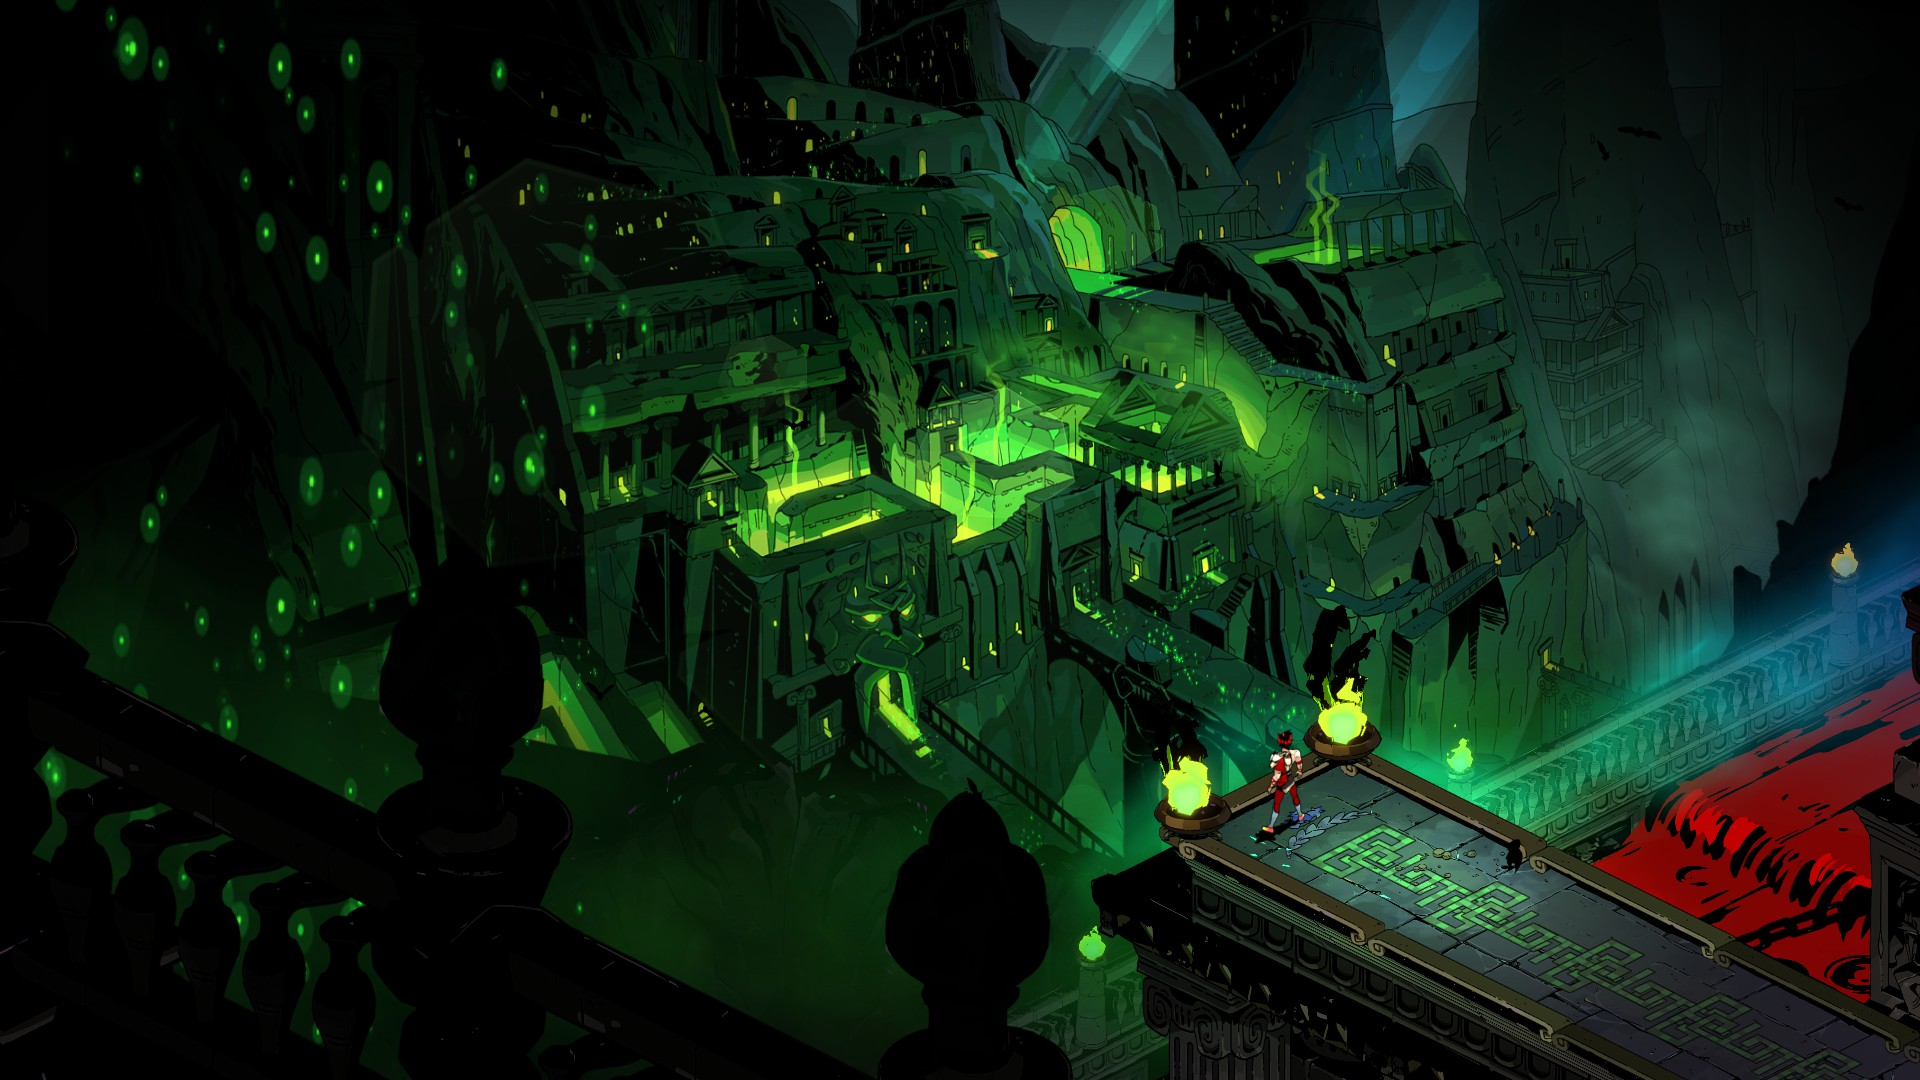
\includegraphics[width=.85\textwidth]{contenu/resources/images/hades}
    \caption{{\it Hades} (2018), Supergiant Games~\cite{supergiant_hades_2018}}
    \label{fig:hades}
\end{figure}

Dans ce contexte de méthodes automatisées, la génération procédurale est un procédé utilisé pour produire toutes sortes de ressources numériques~\cite{smelik_survey_2014}. La génération procédurale est en particulier utilisée pour synthétiser l'apparence visuelle des différents composants des scènes virtuelles~\cite{alessio_procedural_2021}. En combinant des méthodes algorithmiques avec de l'aléatoire, il est possible de générer des cartes de texture qui servent à habiller les mondes virtuels. Une carte de texture désigne une image qui est appliquée sur une surface pour lui donner un aspect visuel dans le but d'accentuer l'immersion des utilisateurs. Différentes textures nécessitent différentes méthodes de synthèse pour être générées. Certains genres de textures sont encore difficilement réalisables avec les méthodes existantes~\cite{lutz_cyclostationary-gaussian_2021}. C'est dans cette perspective que s'inscrit ce travail de recherche, qui a pour but d'approfondir notre compréhension des éléments qui constituent la structure d'une image. La compréhension d'une image et de ces éléments est le sujet d'un autre domaine, le traitement du signal (une image est un signal 2D). Le traitement du signal est un sous-domaine du génie électrique qui étudie la manipulation et l'interprétation des signaux. Nebeker définit le traitement du signal comme étant \og [...] l'ensemble des changements appliqués aux signaux dans le but d'améliorer leur transmission et utilisation. \fg (traduction libre)~\cite{nebeker_fifty_1998}. Quand le signal étudié est une image, le domaine est appelé traitement ou analyse d'image. Afin obtenir une meilleure compréhension de la structure d'une image, ce travail explore l'analyse multi-résolutionnelle locale et son application à la synthèse de texture procédurale. L'analyse multi-résolutionnelle locale est un outil du domaine de l'analyse d'image et est détaillée dans la suite de ce manuscrit au chapitre~\ref{chap:chapitre1}.

\section{Monde virtuel}

Dans le cadre de l'informatique graphique, un monde virtuel est une méthode de représentation de scènes au moyen d'un support numérique. Une scène est une collection d'objets numériques qui interagissent entre eux. Il existe trois sortes d'objets numériques qui composent une scène : de la géométrie, des lumières et des caméras. Avec des algorithmes dits de \og rendu \fg, un monde virtuel peut être converti en image. Les mondes virtuels sont utilisés dans de nombreux domaines~\cite{magnenat-thalmann_introduction_1986}, comme :

\begin{itemize}
    \item le domaine du divertissement, pour les jeux vidéo (l'industrie du jeu-vidéo est un des principaux acteurs des avancées en graphisme) ;
    \item le domaine de l'animation, pour les films d'animation ou les effets spéciaux de films ;
    \item le domaine médical, pour des outils de visualisation de l'anatomie humaine ou de formation en réalité virtuelle ;
    \item le domaine de l'ingénierie, pour aider à la conception d'objets (Conception Assistée par Ordinateur) ou de bâtiments (architecture) ;
    \item le domaine militaire, pour faire des simulations de situations ou des entraînements au combat.
\end{itemize}

\subsection*{Types de rendu}

La visualisation de scènes virtuelles s'opérationnalise au travers d'un logiciel dit \og moteur de rendu \fg utilisant divers algorithmes pour fonctionner~\cite{sherman_chapter_2003}. Un moteur de rendu traite une scène en différentes étapes dans le but de créer une visualisation de cette scène, appelée \og rendu de la scène \fg~\cite{pharr_physically_2023}. Il existe plusieurs méthodes de rendu qui implémentent différents algorithmes pour produire différentes visualisations d'une scène. Pour exécuter leurs calculs, les logiciels de rendu s'appuient sur les capacités des cartes graphiques ({\it Graphics Processing Unit} ou GPU). Les GPUs sont des processeurs hautement parallèles et spécialisés dès leur fabrication pour des calculs graphiques~\cite{das_history_2016}.

\bigskip

\begin{figure}[h]
    \centering
    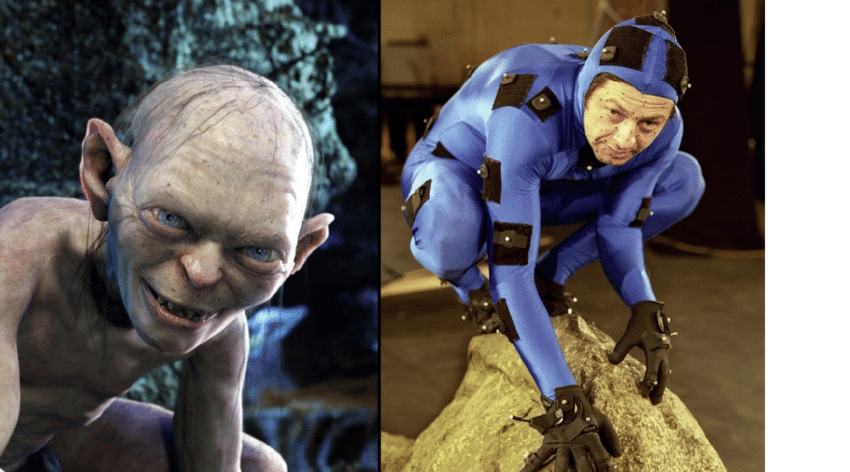
\includegraphics[width=.65\textwidth]{contenu/resources/images/gollum}
    \caption[{\it Gollum} (2002), {\it Le Seigneur des Anneaux : Les Deux Tours}]{{\it Gollum}, personnage complètement généré par image de synthèse par rendu hors-ligne. {\it Le Seigneur des Anneaux : Les Deux Tours}, Peter Jackson~\cite{jackson_lord_2002}. Image par Mou~\cite{mou_keyframe_2018}.}
    \label{fig:gollum}
\end{figure}

Les méthodes de rendu peuvent être séparés en deux grandes catégories : le rendu \og hors-ligne \fg et le rendu \og en temps-réel \fg. Le rendu hors-ligne désigne les algorithmes qui font la visualisation de scènes non interactives, où il n'est pas possible de contrôler les interactions entre les éléments de la scène. Les films d'animation ou les effets spéciaux de films~\ref{fig:gollum} sont des exemples de rendus fait hors-ligne. L'utilisation de méthodes de rendu hors-ligne est en fait devenu une norme dans l'industrie cinématographique~\cite{media_history_2021}, car elle permet la création de scènes qu'il serait impossible de tourner à l'aide de caméras traditionnelles. À l'inverse, lors d'un rendu en temps-réel, une personne utilisatrice a un contrôle sur la scène qui est rendue pendant qu'elle est rendue. Le déplacement d'un personnage dans un jeu-vidéo, la manipulation d'un modèle de pont dans un logiciel d'architecture et l'affichage d'objets dans une application de réalité augmentée sont tous des exemples de rendus en temps-réel. Une même scène peut être rendue avec plusieurs méthodes de rendu, la visualisation finale sera alors différente à chaque fois. Une scène rendue en temps-réel d'une part et hors-ligne d'autre part, est montrée à la figure~\ref{fig:zero-day}. Les enjeux et contextes des rendus hors-ligne et en temps-réel diffèrent. Le travail présenté dans ce manuscrit s'intéresse aux méthodes de rendu en temps-réel. Dans la méthode proposée, bien qu'une partie de préparation des données soit nécessaire, le rendu final se fait en temps-réel. Les problématiques et solutions concernant le rendu hors-ligne ne sont donc pas abordées dans ce travail.

\bigskip

\begin{figure}[h]
    \centering
    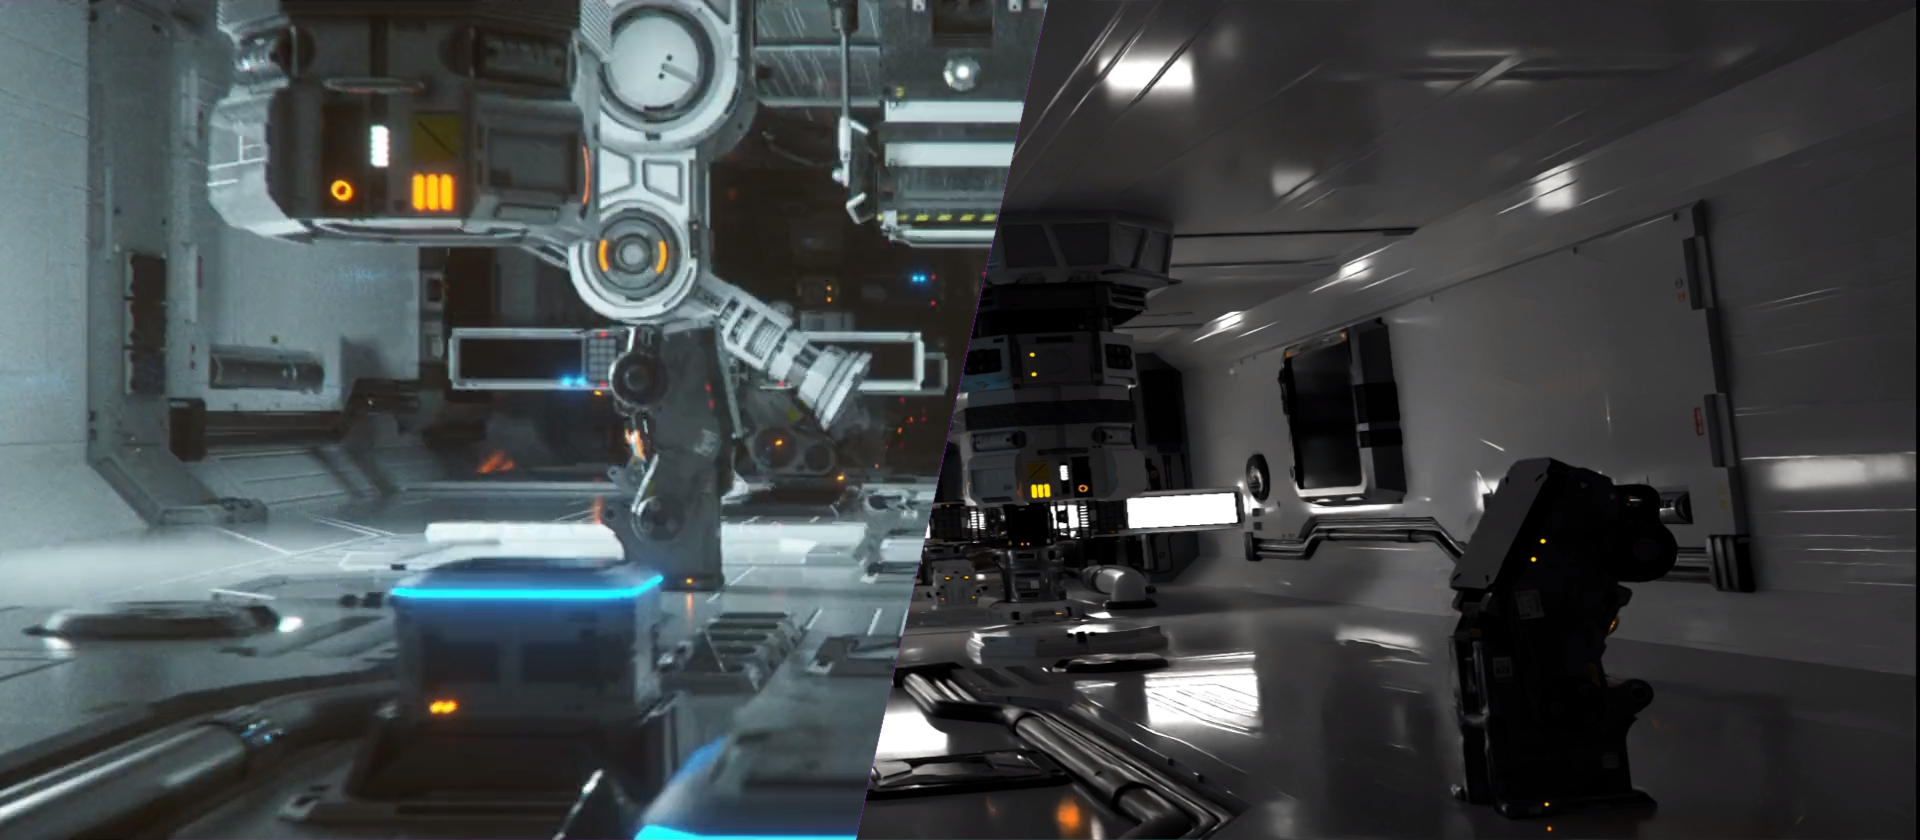
\includegraphics[width=\textwidth]{contenu/resources/images/zero_day_comparison}
    \caption[{\it Zero-Day} (2015), BEEPLE]{{\it Zero-Day} (2015), BEEPLE. À gauche rendu original hors-ligne, à droite rendu temps-réel par SY tracé de chemins, NVIDIA~\cite{ZeroDay}}
    \label{fig:zero-day}
\end{figure}

Une méthode de rendu en temps-réel doit répondre à certaines contraintes dues à la nature interactive de la scène. Le rendu de la scène ne peut pas se faire en avance, car la scène est modifiée pendant l'utilisation. Le rendu doit être assez rapide pour afficher les images assez vite de telle sorte que le flux soit continu à l'œil humain. L'industrie cinématographique utilise un standard de 24 images par secondes pour l'enregistrement de films~\cite{deguzman_why_2023}. Pour un rendu en temps-réel, les applications visent des objectifs d'au moins 30 ou 60 images par secondes, afin que le contrôle utilisateur soit confortable~\cite{janzen_is_2014}. Les algorithmes utilisés doivent ainsi être conçus pour s'exécuter avec moins de temps, moins de ressources de calcul, et moins d'espace mémoire disponible.

\subsection*{Maillage}

Pour manipuler une scène virtuelle, il est nécessaire d'avoir une représentation des éléments qui la composent. Une représentation est une manière technique de décrire et stocker les données d'une scène. Il y a deux façons de représenter une géométrie dans un monde virtuel. Les représentations continues, comme les surfaces implicites, se rapprochent au mieux des formes des objets du monde réel, mais sont difficiles à créer. Les représentations discrètes, comme les maillages, approximent les représentations continues par des ensembles de polygones~\cite{coons_surfaces_1967}, souvent des triangles. Les polygones qui forment un maillage sont définis explicitement par des données géométriques, notamment les positions des sommets et les sommets des faces. La figure~\ref{fig:procedural-mesh} montre les polygones qui composent un modèle de terrain. Dans ce travail, seuls les maillages seront utilisés. Les maillages sont des structures habituelles dans les mondes virtuels.

\begin{figure}[h!]
    \centering
    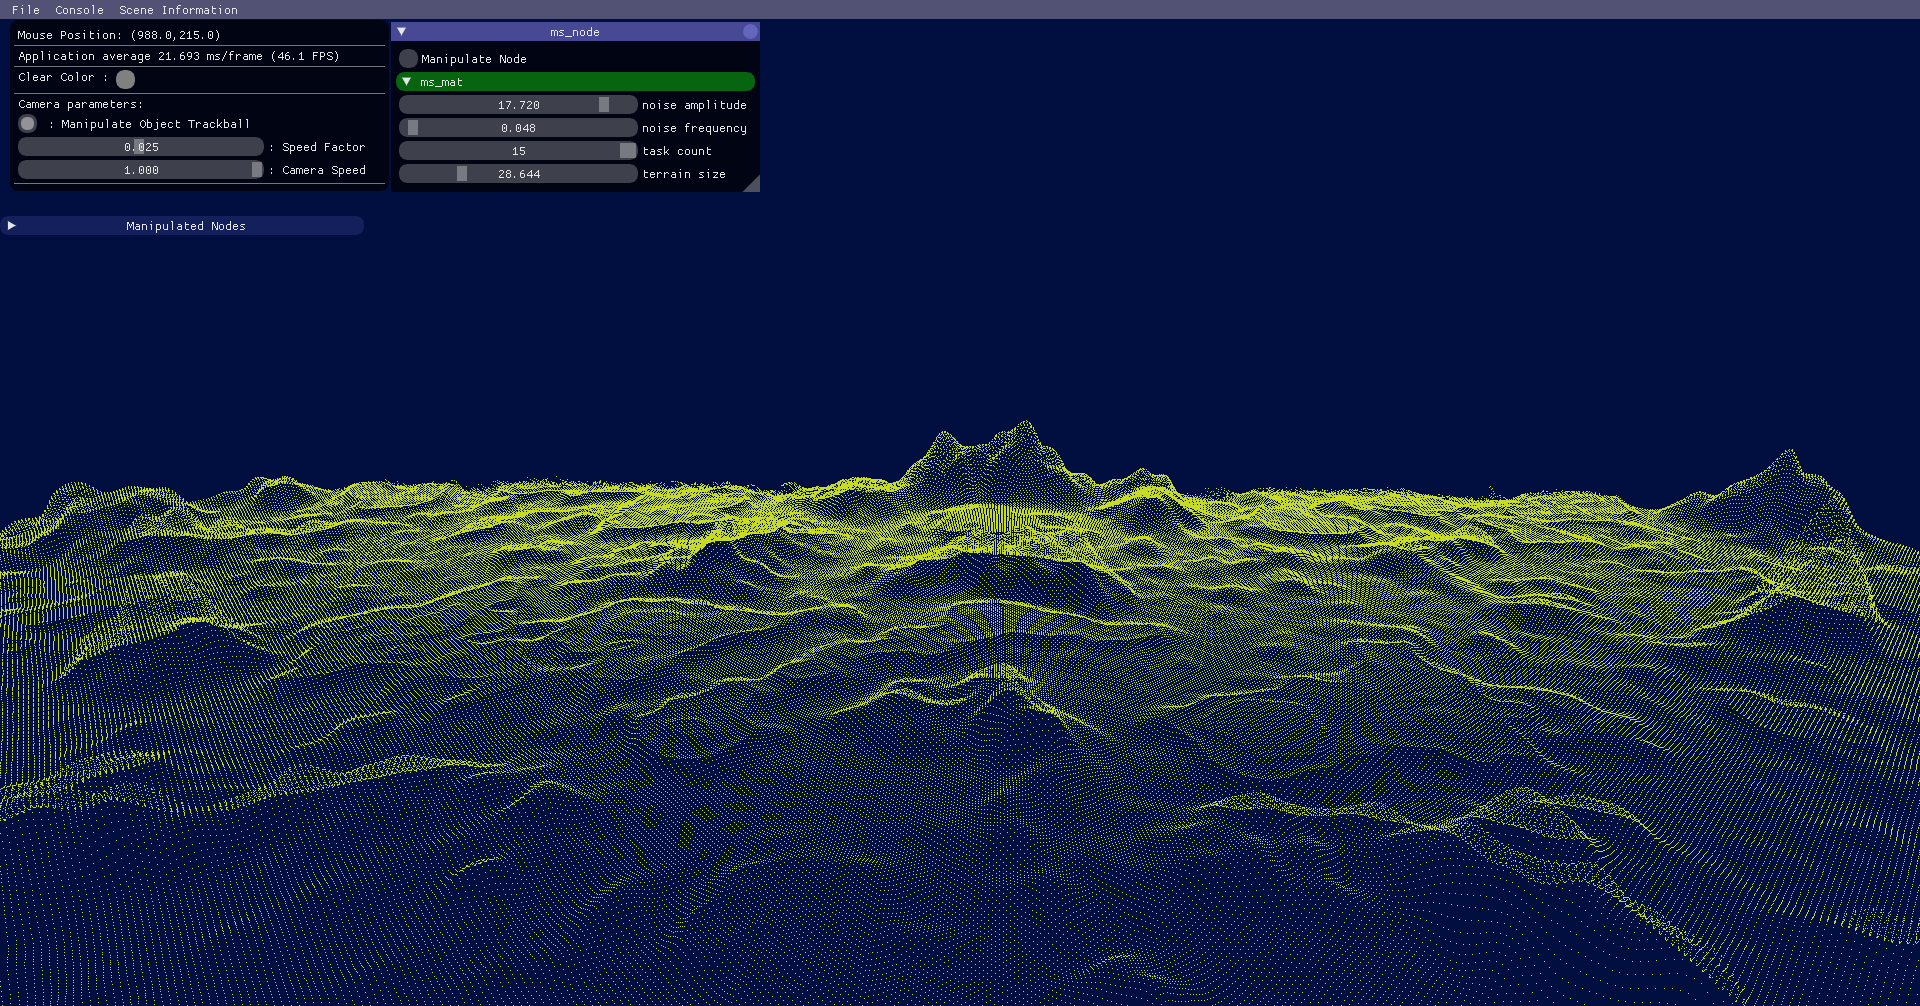
\includegraphics[width=\textwidth]{contenu/resources/images/full_terrain}
    \caption{Maillage d'un terrain généré procéduralement}
    \label{fig:procedural-mesh}
\end{figure}

\section{Texture}

\subsection*{Plaquage de texture}

Le maillage utilisé pour représenter une géométrie est une approximation. Pour affiner la géométrie, ou lui attribuer une apparence, il est possible d'utiliser des \og textures \fg. Une texture est une fonction d'un espace de coordonnées, habituellement à deux ou trois dimensions, à valeurs dans un espace quelconque qui représente les différents attributs possibles de la texture. Les dimensions de l'espace d'arrivée sont appelées \og canaux \fg de la texture. Les textures représentent généralement la couleur d'une surface, ou d'autres grandeurs physiques comme la profondeur ou l'élévation, qui servent au rendu de la géométrie à laquelle est associée la texture. En fonction du modèle de rendu choisi pour la scène, différentes textures sont nécessaires. Le format de rendu physique réaliste ({\it Physically Based Rendering} ou PBR), standard de l'industrie~\cite{hoffman_siggraph_2010}, nécessite typiquement cinq cartes de texture~\cite{pharr_physically_2023} : l'albedo (ou couleur), mais aussi la normale, la hauteur, la rugosité et l'occlusion ambiante.

\bigskip

\begin{figure}
    \centering
    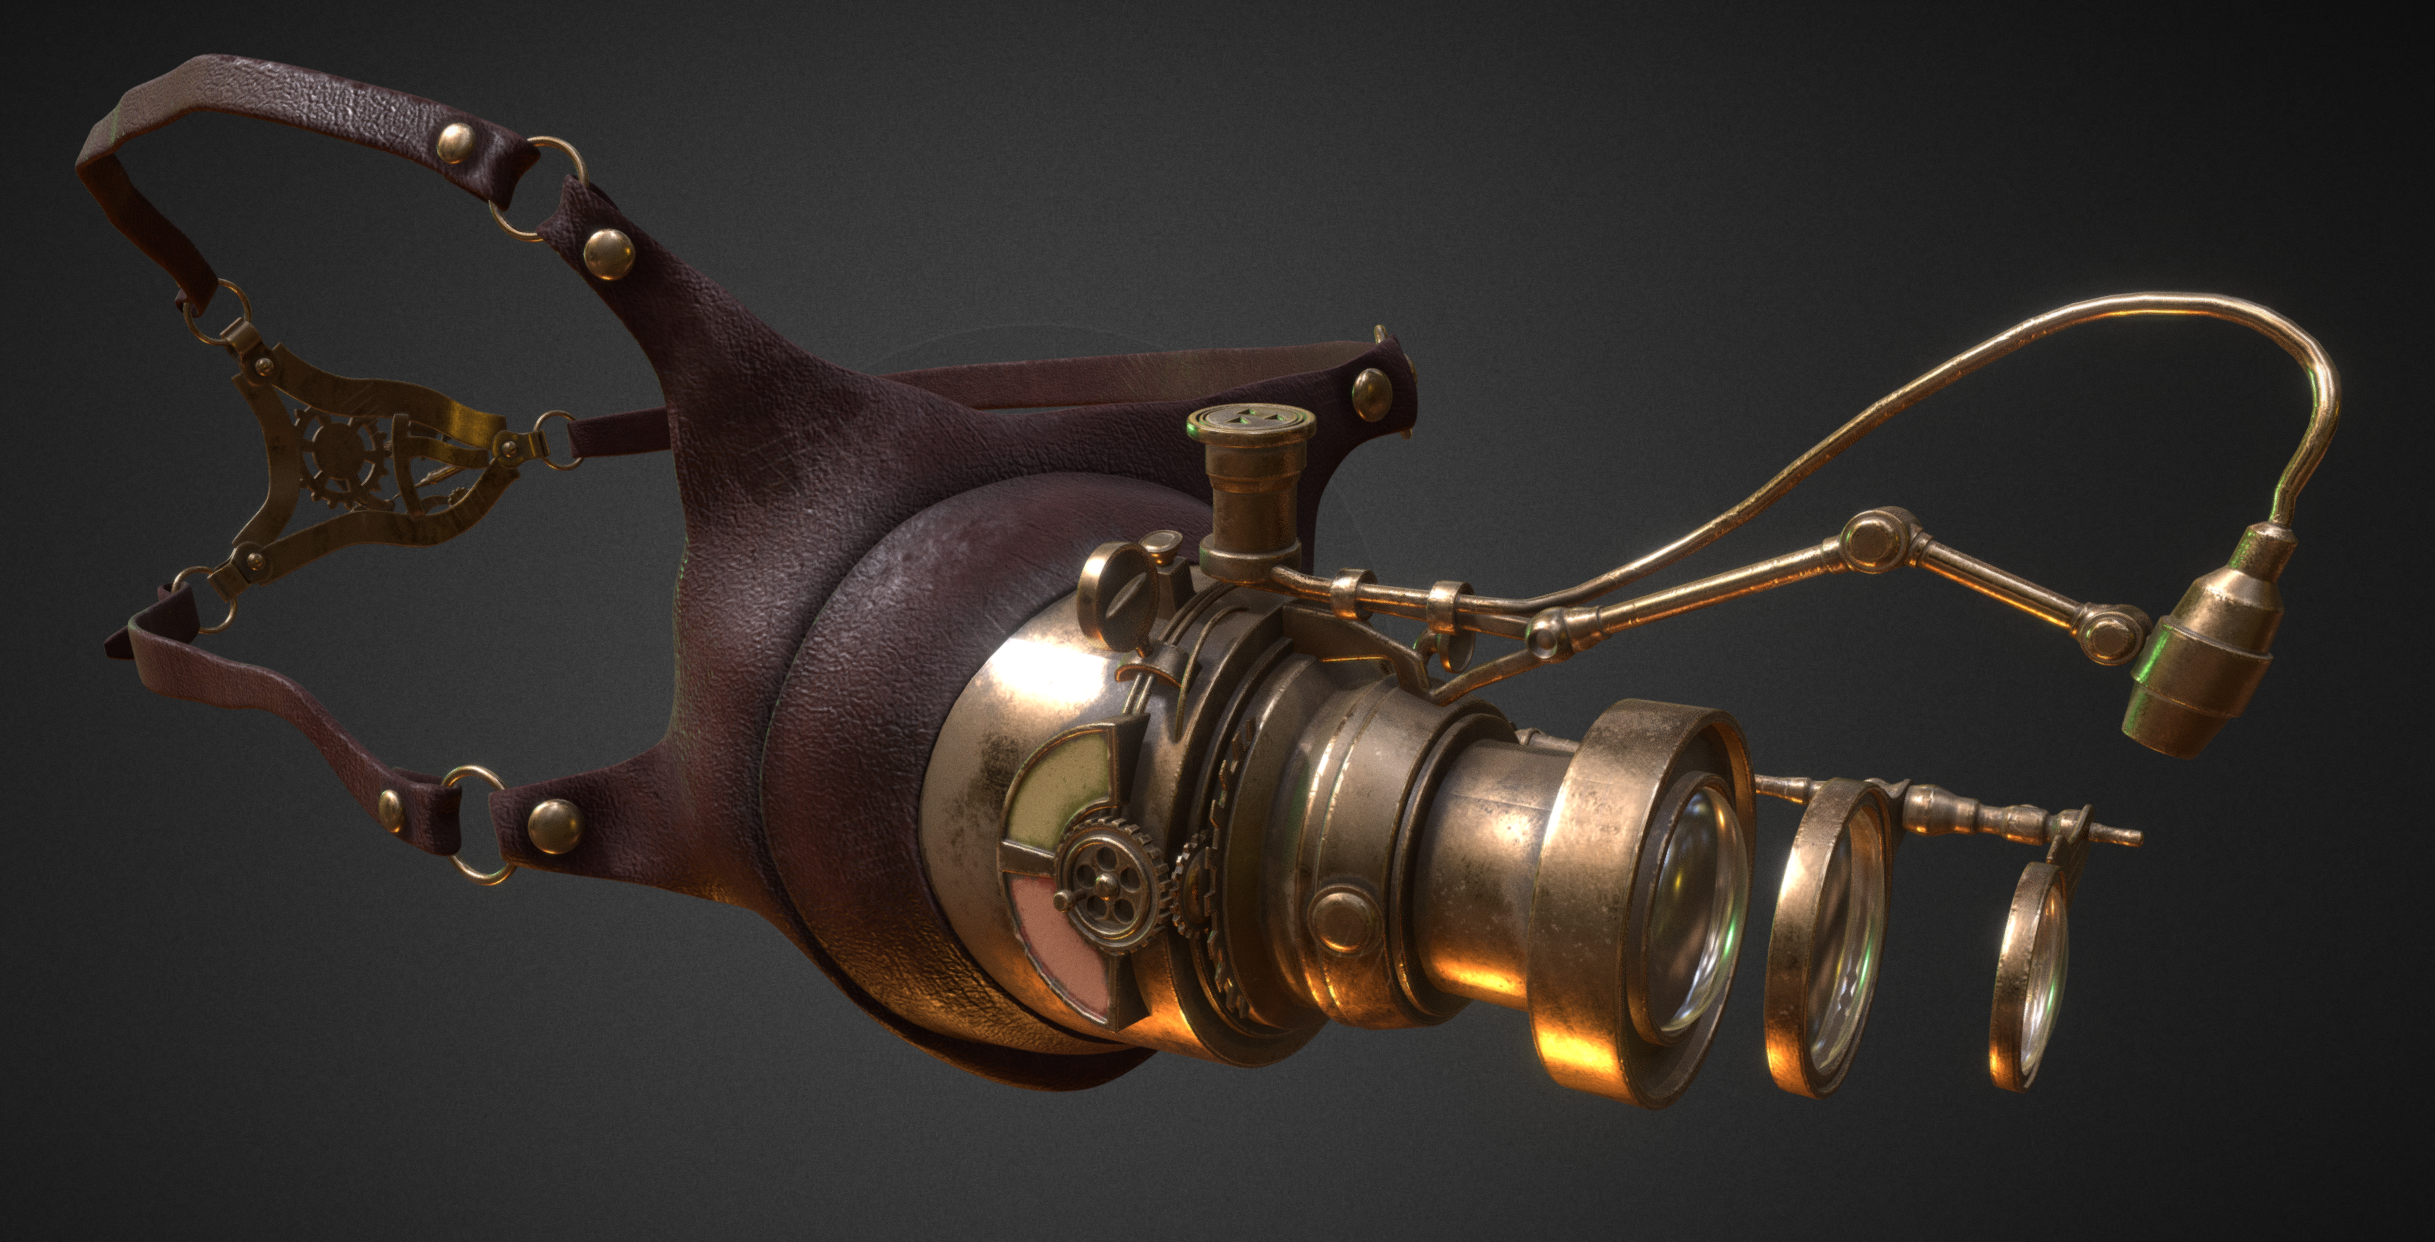
\includegraphics[width=.65\textwidth]{contenu/resources/images/mutli-material-object}
    \caption[Rendu d'un objet comportant plusieurs matériaux]{Plusieurs matériaux différents sont utilisés pour le rendu de cet objet~\cite{fig:multi-material}}
    \label{fig:multi-material}
\end{figure}

La méthode de travail usuelle en industrie consiste à regrouper ces différentes textures, ainsi que le modèle d'éclairage, dans une ressource dite \og matériau \fg. Les objets d'une scène sont composés de plusieurs matériaux, qui présentent chacun des propriétés physiques différentes. Dans la figure~\ref{multi-material} par exemple, la lunette a un harnais en cuir, un objectif en métal et des lentilles en verre. Pour créer leurs scènes, les artistes façonnent leurs objets en commençant par la géométrie, avant de créer (ou réutiliser) différents matériaux pour habiller leurs objets.

\bigskip

Il existe deux méthodes classiques de stockage pour une texture : procédurale ou discrète. Une texture procédurale est représenté sous une forme fonctionnelle, à l'aide d'équations ou de procédures. Une texture discrète, quant à elle, est stockée comme une image numérique, c'est-à-dire un tableau discret et fini de données. La représentation procédurale, dont un exemple est donné à la figure~\ref{fig:perlin-noise}, présente plusieurs avantages par rapport à la représentation discrète :

\begin{itemize}
    \item la compacité : pour stocker une texture procédurale, il suffit de stocker les fonctions ou chaines d'instructions qui la définissent. Une texture procédurale n'occupe donc que très peu d'espace en mémoire.
    \item la taille : une texture procédurale est définie comme une fonction sur un espace de paramètre. Une texture procédurale est donc intrinsèquement infinie.
    \item la résolution : une texture procédurale est une fonction continue au sens mathématique. Il est possible de connaître la valeur exacte d'une texture procédurale en n'importe quel point de l'espace de coordonnées en l'évaluant en ce point.
\end{itemize}

Les textures procédurales ont cependant des désavantages. Certaines apparences souhaitées sont difficilement exprimables de manière fonctionnelle. Une expression fonctionnelle peut aussi être difficile à manipuler pour des artistes, puisqu'il faut ajuster des paramètres et modifier l'apparence de manière indirecte. De plus, l'expression d'une texture procédurale est parfois complexe et peut être un enjeu pour la synthèse en temps-réel. Il arrive que la fonction ou suite d'instructions qui définissent une texture procédurale sont si longs à exécuter que le budget de temps pour le rendu de l'image est dépassé. Une texture qui fait dépasser le budget temps du rendu n'est pas viable.

\bigskip

\begin{figure}[h]
    \centering
    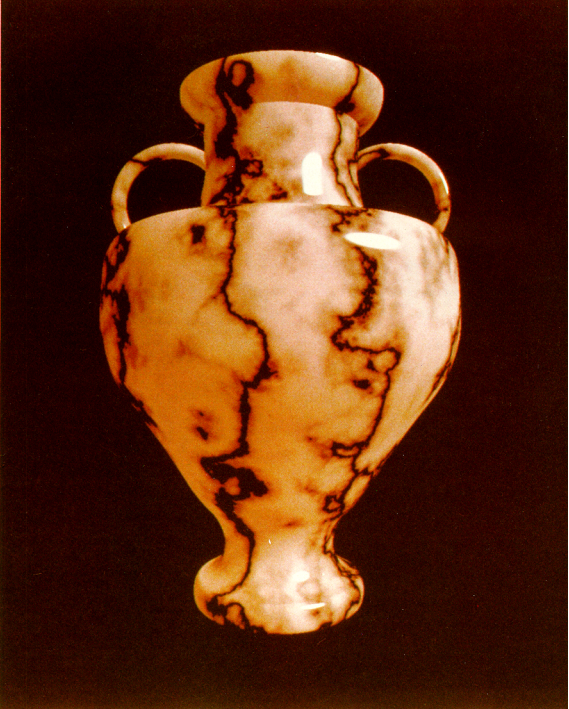
\includegraphics[width=.5\textwidth]{contenu/resources/images/perlin-noise}
    \caption[Bruit de Perlin]{La notion de texture procédurale est introduite par Ken Perlin en 1985 avec son bruit de Perlin~\cite{perlin_image_1985}.}
    \caption{fig:perlin-noise}
\end{figure}

Résoudre les problématiques des textures procédurales est un enjeu de l'informatique graphique. Obtenir de nouvelles apparences, avoir un meilleur contrôle par les artistes et une évaluation plus rapide sont des sujets constamment explorés dans le domaine~\cite{heitz_high-performance_2018, tricard_procedural_2019, lutz_cyclostationary-gaussian_2021, baldi_differentiable_2023}. Le sujet présenté dans ce manuscrit s'inscrit dans la problématique de l'agrandissement du champ des apparences représentables par texture procédurale.

\subsection*{Échantillonnage}

Le processus utilisé traditionnellement pour le rendu en temps-réel est appelé le \og \textit{pipeline} graphique de rastérisation \fg. Dans ce \textit{pipeline}, la scène rendue est projetée sur le plan image, qui est une représentation virtuelle de l'écran. La géométrie est ensuite divisée en petits éléments de surface appelés \og fragments \fg, durant l'étape éponyme de \og rastérisation \fg. La figure~\ref{fig:rasterization} montre comment un triangle est rastérisé dans le \textit{pipeline} traditionnel. Les fragments sont les éléments atomiques du \textit{pipeline} de rastérisation : ce sont les plus petits éléments indivisibles manipulés. Au terme du processus de rendu, un fragment est soit défaussé car non visible dans l'image finale, soit donné une couleur et affiché. Un fragment affiché à l'écran est appelé un \og pixel \fg (mot-valise de \textit{Picture Element}). L'ensemble des pixels forme l'image rendue.

\begin{figure}[h]
    \centering
    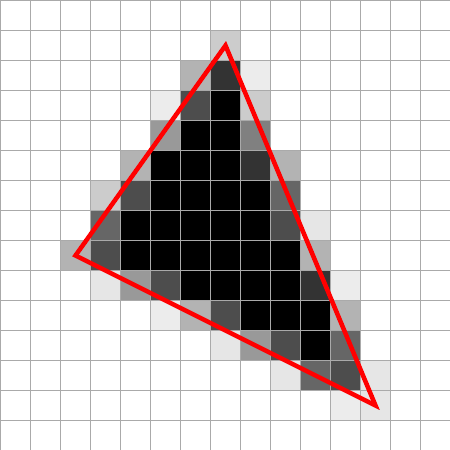
\includegraphics[width=.55\textwidth]{contenu/resources/images/rasterization}
    \caption[Rastérisation d'un triangle]{Un triangle (rouge) rastérisé (noir). Crédit à Wojciech mula pour l'image.}
    \label{fig:rasterization}
\end{figure}

\bigskip

\begin{figure}
    \centering
    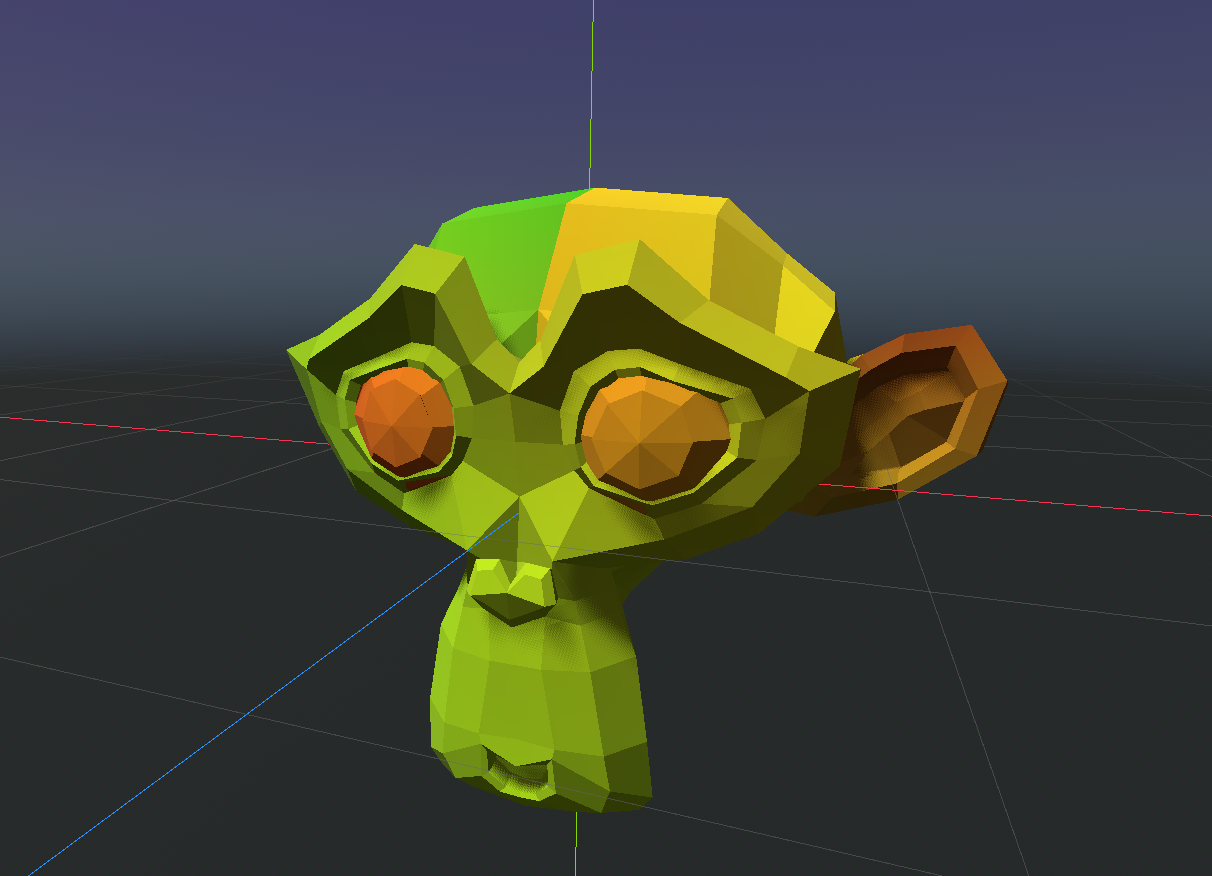
\includegraphics[width=.55\textwidth]{contenu/resources/images/uv_suzanne}
    \caption[Coordonnées UV du modèle Suzanne]{Visualisation des coordonnées UV de Suzanne~\cite{suzanne-uv}, modèle 3D de référence du logiciel Blender}
    \label{fig:uv-suzanne}
\end{figure}

Pour appliquer une texture à une géométrie, un système de coordonnées, dites \og coordonnées UV \fg, est utilisé. Les coordonnées UV sont des vecteurs 2D, entre $(0, 0)$ et $(1, 1)$. Les sommets des maillages des objets de la scène ont chacun des coordonnées UV, qui leurs sont associées à la création de l'objet. Les coordonnées UV sont ensuite interpolées entre les sommets lors de la rastérisation. Les fragments ont ainsi chacun des coordonnées UV. Un exemple de rendu exhibant les coordonnées UV d'un modèle 3D est montré à la figure~\ref{fig:suzanne}. Les coordonnées UV indiquent quelles parties de la texture correspondent à chaque fragment de la géométrie. L'action d'évaluer une texture en utilisant les coordonnées UV des fragments est appelée \og échantillonnage \fg de la texture. Ce processus d'échantillonnage s'effectue en général au moment du rendu.

\subsection*{Filtrage}
\label{subsec:filtering}

L'étape d'échantillonnage comporte un problème inhérent, dû au fonctionnement d'un écran et à la nature discrète du système de pixels. Comme expliqué, la géométrie de la scène est projetée, puis découpée en fragments. Le fragment représente donc une partie de surface continue. Mais un fragment est un élément discret, il ne prend qu'une seule valeur. Le schéma en figure~\ref{fig:aliasing} illustre cette problématique. Avec les notations de la figure, un fragment $P$ représente la surface projetée $e(P)$ avec une seule valeur. La valeur que devrait prendre le fragment est l'intégrale de la texture sur l'empreinte $e(P)$. Cette valeur est cependant difficile à calculer dans la majorité des cas. Dans le cas de textures discrètes, une considération supplémentaire doit être faite. L'empreinte du fragment sur la surface texturée est souvent de taille différente que le texel (mot-valise de \textit{Texture Element}) de la texture.

\bigskip

\begin{figure}
    \centering
    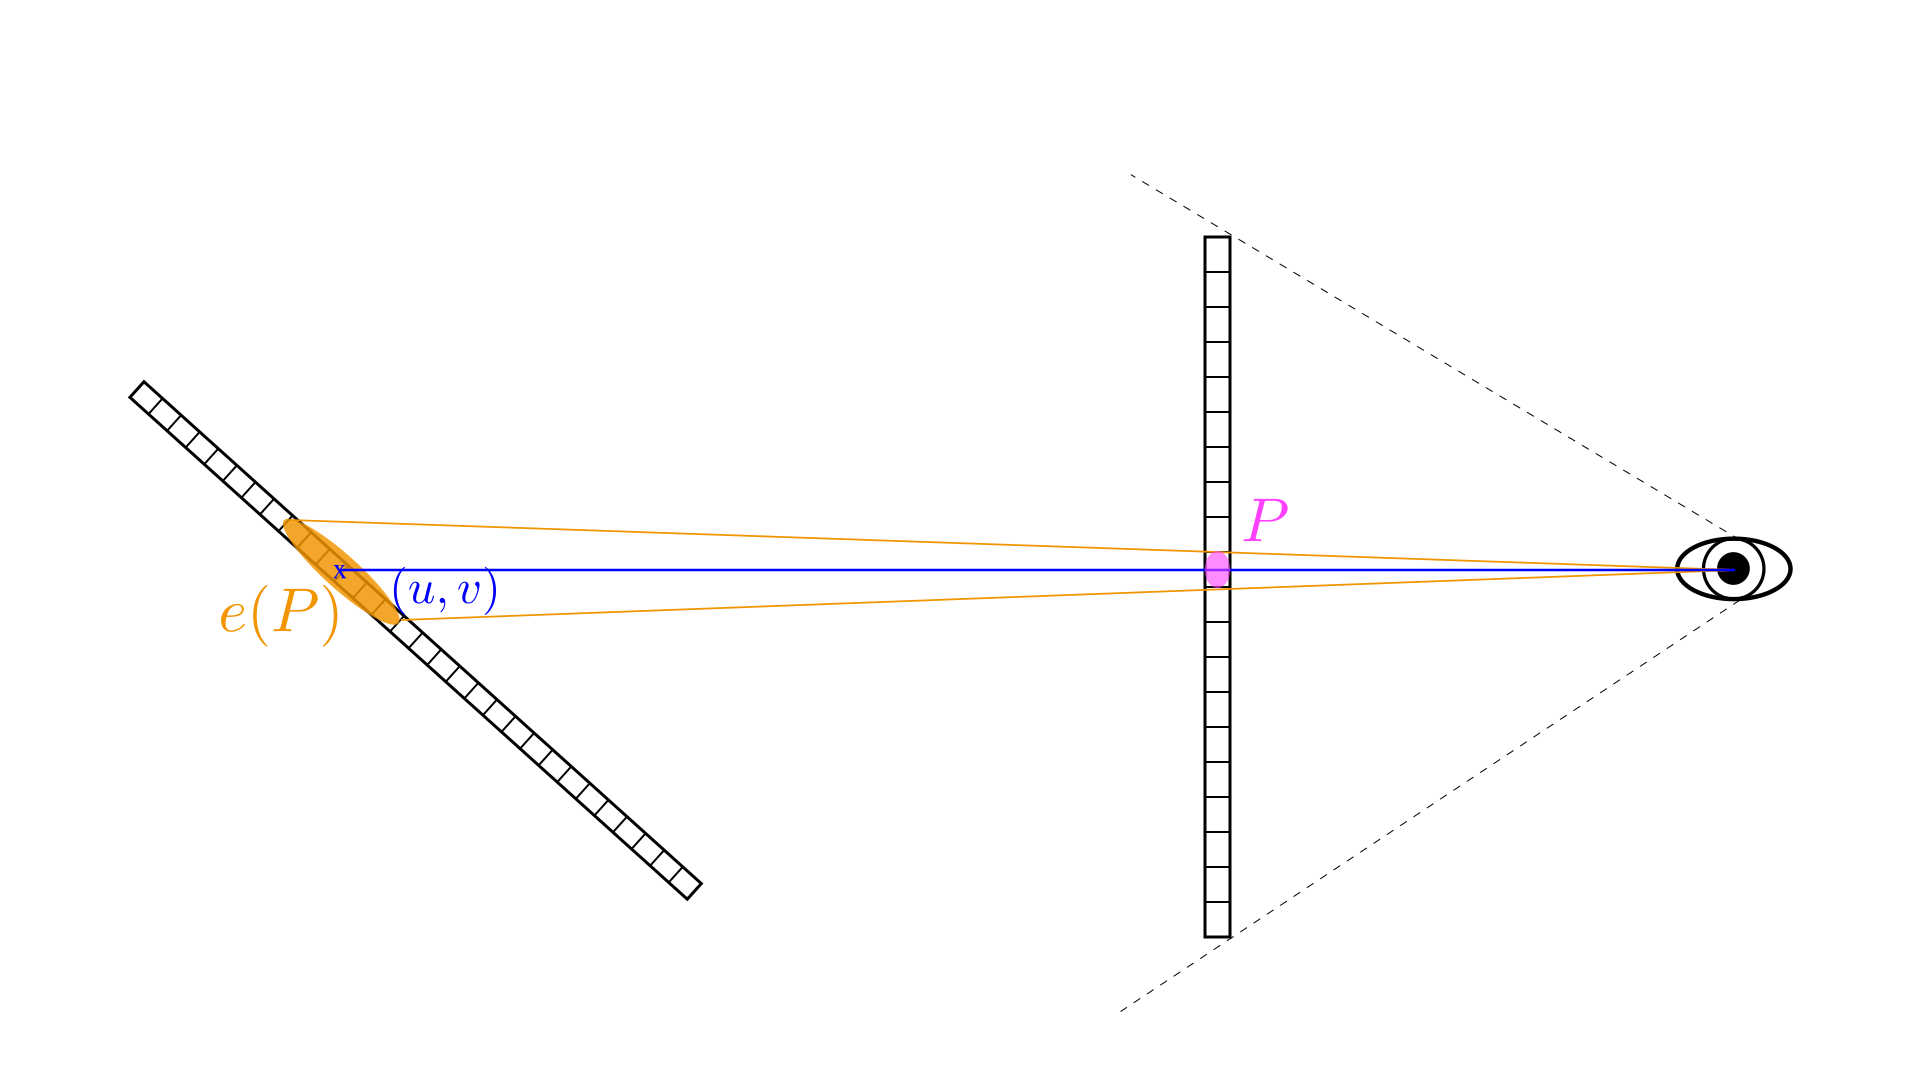
\includegraphics[width=\textwidth]{contenu/resources/images/schema_filtrage}
    \caption[Visualisation du problème d'échantillonnage lors du rendu par rastérisation]{À cette distance de l'écran, l'empreinte $e(P)$ du fragment sur la surface texturée couvre plusieurs texels. Les coordonnées $(u, v)$ ne sont pas suffisantes pour capturer toute l'information de la texture.}
    \label{fig:aliasing}
\end{figure}

Les comportements indésirables causés lors des étapes de rendu et observables sur l'image finale sont appelés \og artefacts de visualisation \fg. Dans le cas de l'échantillonnage, les artefacts causés par la différence de taille entre un fragment et son empreinte sur une surface texturée sont appelés artefacts d' \og aliassage \fg. Pour résoudre les problèmes d'aliassage, plusieurs méthodes dites de \og filtrage \fg sont utilisées, dépendamment du problème d'aliassage rencontré :

\begin{itemize}
    \item le \og sur-échantillonnage \fg signifie que l'empreinte d'un fragment est plus petite qu'un texel. En cas de sur-échantillonnage, plusieurs fragments voisins peuvent prendre la même valeur. Avoir une même valeur pour plusieurs fragments voisins donne un aspect crénelé à l'image et les contours des objets sont en escalier. La solution idéale dans ce cas est d'augmenter la résolution de la texture utilisée ; ce n'est cependant pas tout le temps possible. Une alternative commune est de faire l'interpolation des valeurs des quatre texels voisins. La texture est échantillonnée quatre fois pour chaque fragment et l'image prend un aspect légèrement flouté, mais l'effet escalier est réduit. Un exemple est montré à la figure~\ref{fig:filtering}
    \item le \og sous-échantillonnage indique que l'empreinte d'un fragment est plus grande qu'un texel et en recouvre plusieurs, comme à la figure~\ref{fig:aliasing}. En cas de sous-échantillonnage, des fragments voisins représentent du contenu éloigné spatialement sur la surface. La surface entre les centres des empreintes de fragments voisins est alors mal représentée. De loin, la surface texturée présente des motifs dits de \og moiré \fg. Des bandes non-présentes dans la texture apparaissent sur le rendu et il y a un effet de scintillement lorsque la caméra est déplacée dans la scène. L'apparence souhaitée est l'intégrale des texels qui sont sous l'empreinte du fragment, mais un algorithme de rastérisation naïf ne lit qu'un seul texel. La solution idéale serait de calculer l'intégrale sur tous les texels couverts par l'empreinte du fragment. Calculer l'intégrale directement est souvent irréalisable. L'approche traditionnelle dite \og filtrage tri-linéaire \fg consiste à pré-calculer une approximation de l'intégrale pour différentes tailles d'empreintes et trouver le bon niveau au moment du rendu. Cette approche double l'occupation mémoire pour chaque texture, mais les effets de moiré disparaissent.

%    \item Différentes résolution des textures utilisées appelées \og MIPs maps \fg sont pré-calculées avant le rendu. Ces MIPs maps sont l'approximation des intégrales de régions de texels de différentes tailles. La technique de filtrage dit \og tri-linéeaire \fg consiste à trouver les niveaux adéquats de MIPs maps auquel l'empreinte du fragment a une taille similaire à un texel. L'échantillonnage de la texture se fait alors dans les deux niveaux les plus proches.
%    \item L'alternative classique consiste à pré-calculer différentes échelles de la texture utilisée, appelées \og MIP maps \fg, et de trouver l'échelle adéquate de telle sorte qu'un texel ait la même taille qu'un fragment. L'échantillonnage est plus lourd et on prend plus d'espace mémoire pour stocker les MIP maps, mais la texture est mieux rendue de loin.
\end{itemize}

\bigskip

\begin{figure}
    \centering
    \begin{subfigure}[b]{.45\textwidth}
        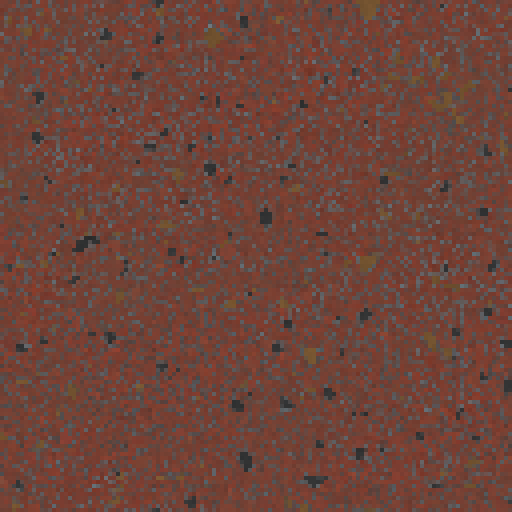
\includegraphics[width=\textwidth]{contenu/resources/images/porcelain_no_filter}
        \caption{Sans filtrage}
    \end{subfigure}
    \hfill
    \begin{subfigure}[b]{.45\textwidth}
        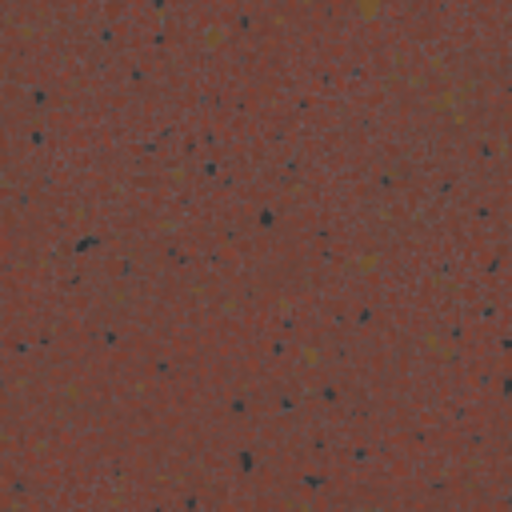
\includegraphics[width=\textwidth]{contenu/resources/images/porcelain_filter}
         \caption{Avec filtrage linéaire}
     \end{subfigure}
    \caption{Filtrer correctement est un enjeu majeur dans l'utilisation des textures}
    \label{fig:filtering}
\end{figure}

S'assurer de filtrer correctement lors de l'échantillonnage est un enjeu majeur pour obtenir un rendu fidèle aux textures utilisées. C'est particulièrement le cas lors la création de textures procédurales, qui est le sujet de cette étude. Diverses méthodes peuvent être utilisées pour la création de textures procédurales. S'assurer de la filtrabilité d'une méthode de création de textures est une des problématiques principales et un critère de qualité de la synthèse de texture, présentée dans la section suivante.

%{\color{red}Pertinence de ce paragraphe ?}
%De nombreuses méthodes de filtrage plus élaborées sont employées pour obtenir des résultats de meilleure qualité, ou pour filtrer des textures plus compliquées. Par exemple quand les textures ne sont plus des images prédéterminées à l'avance, mais qu'elles sont générées au moment du rendu.
% oui pertinent, mentionner les autres solutions "idéales" mais plus difficiles (voir not). filtre analytique et pré-intégration
%OU p-e supprimer paragraphe

\section{Synthèse de texture}

De nombreuses surfaces texturées lors d'un rendu, comme des sols, sont de grande taille. Comme discuté précédemment~\ref{subsec:filtering}, produire des textures de résolution suffisante pour texturer de grandes surfaces sans artefacts demande une grande occupation mémoire et un long temps de création. Étirer les textures en utilisant les coordonnées UV est une solution, qui atteint cependant ses limites assez rapidement. Utiliser une texture de plus basse résolution cause des artefacts visuels. Il est possible de résoudre le problème en créant directement une texture de taille adaptée à la surface à couvrir, procédé appelé \og synthèse de texture \fg. Par extension, une texture générée par un algorithme de synthèse est aussi appelée une synthèse. Les textures représentent des apparences visuelles de matériaux diverses. Il est possible de classifier des textures de plusieurs manières différentes. Une façon commune de classifier des textures est d'opposer les textures stochastiques, dont les couleurs de pixels semblent aléatoires, et les textures régulières, qui présentent une répétition régulière de motifs~\cite{lieu_near-regular_2004}.

\bigskip

\begin{figure}[H]
    \centering
    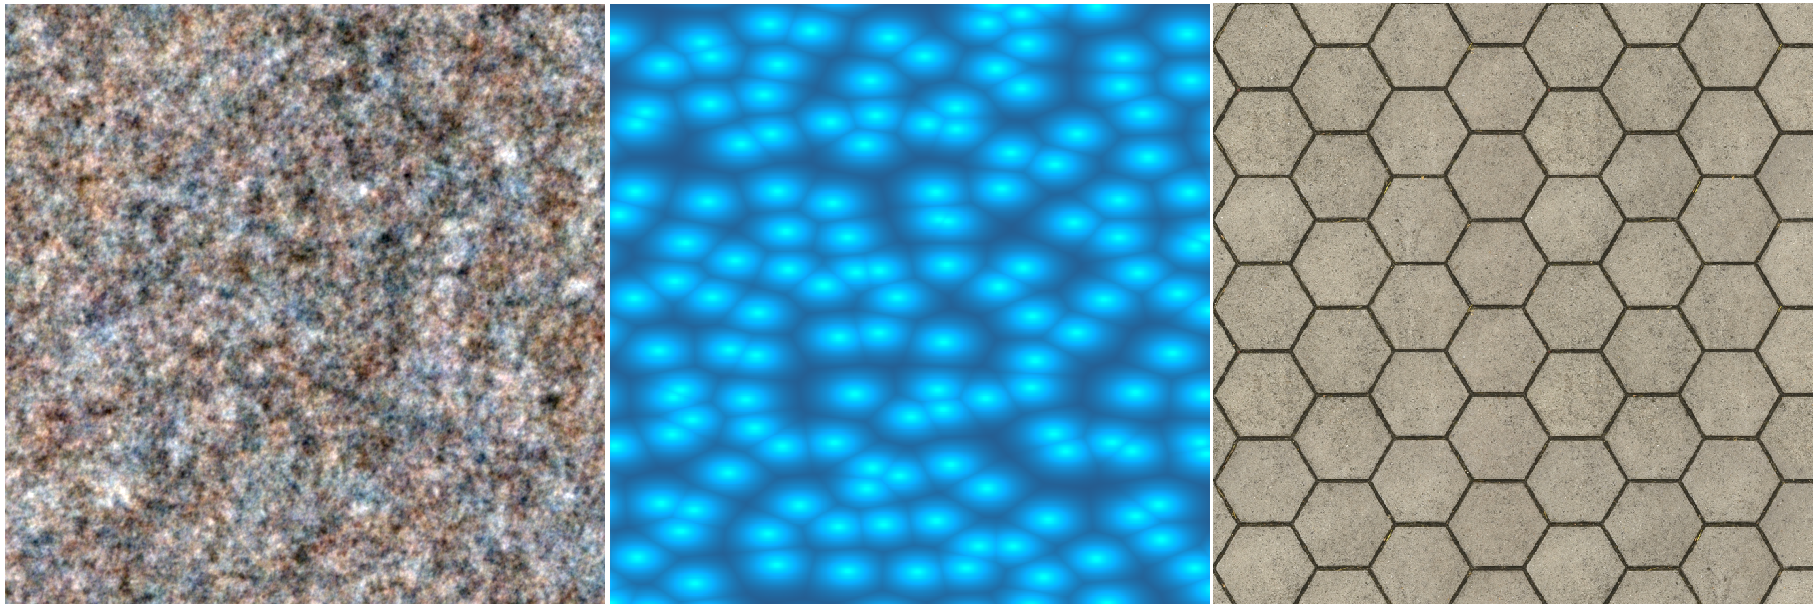
\includegraphics[width=\textwidth]{contenu/resources/images/structure_scale}
    \caption[Classification des textures selon leur niveau de structure]{Les textures peuvent être classées selon leur niveau de structure : stochastiques ou gaussiennes (gauche), semi-régulières (milieu), ou structurées (droite)}
    \label{fig:échelle-structure}
\end{figure}
% TODO remplacer image de droite par image pote Loucas

Le travail présenté dans ce manuscript s'intéresse cependant à la synthèse de texture présentant de la structure. Le concept de structure, bien qu'intuitif, est difficile à définir de manière formelle. Dans le cadre de ce manuscript, la \og structure \fg d'une texture désigne comment les différentes parties de la structure sont agencées les unes par rapport aux autres. Dans une texture structurée, les éléments de la texture forment certains schémas ou présentent une certaine forme de régularité. La classification de textures utilisée dans ce travail est faite selon le niveau de structure des textures car c'est le thème central de l'étude. La figure~\ref{fig:échelle-structure} illustre la classification proposée.

\subsection*{Algorithme de synthèse}

Une synthèse de texture un procédé qui permet de produire une texture de taille arbitraire, pouvant prendre en argument des paramètres de différente nature. Différentes synthèses possèdent différentes propriétés, qui peuvent être voulues ou non en fonction de la scène à rendre. Par exemple la texture générée est souvent infinie, il est possible de l'appliquer à des surfaces de taille quelconque avec la résolution désirée. De plus, la texture est évaluée au vol (pendant le rendu) et n'a pas besoin d'être stockée en mémoire. Cela réduit l'occupation mémoire de la texture.

\bigskip

Il existe plusieurs types de synthèses différentes, qui produisent des types de textures différentes. Une première distinction majeure qui est souvent faite est, comme pour le rendu, entre une synthèse hors-ligne et une synthèse en temps réel. Les ressources en temps et en puissance de calcul impliquées diffèrent, les enjeux ne sont pas les mêmes. Les travaux proposés étudient le rendu et la synthèse temps-réel, les synthèses hors-lignes comme les synthèses par optimisation ou par apprentissage profond ne seront pas abordées. Les algorithmes étudiés ici ont la contrainte de devoir s'exécuter au vol, sans que le budget de temps du rendu dépasse le seuil établi. Pour rentrer dans ces contraintes de temps, les méthodes de synthèse exploitent la puissance des GPUs, notamment leur aspect hautement parallélisable. Les algorithmes de synthèse doivent s'exécuter de manière parallèle et chaque fragment doit se calculer indépendamment de ses voisins.

\subsection*{Synthèse temps-réel} % / Types de synthèse

Sous ces contraintes d'efficacité et de rapidité, de nombreux algorithmes subsistent ; deux grandes catégories de méthodes courantes sont la synthèse \og par réorganisation \fg et la synthèse \og par convolution \fg.

\subsubsection{Synthèse par réorganisation}

Le but d'une synthèse par réorganisation est de reproduire un extrait de texture donné en entrée en réutilisant et réagençant son contenu. Dans une synthèse par réorganisation, le contenu est découpé en petites régions connexes dites « tuiles ». Plusieurs paramètres comme la taille, forme et disposition des tuiles peuvent être modifiés pour varier la synthèse. L'exemple le plus simple de synthèse par réorganisation est le pavage périodique. Dans un pavage périodique, la texture d'entrée est simplement répétée jusqu'à couvrir la surface désirée. Pour pouvoir faire un pavage périodique, il faut que la texture d'entrée soit périodique, c'est-à-dire qu'elle se répète sans coupure. Le pavage périodique, bien que très rapide, est de faible qualité. Des artefacts visuels sont induits, car il n'y a aucune variation au sein de la texture générée et les motifs sont répétés très régulièrement. Quelques exemples d'artefacts visuels causés par un pavage périodique sont montrés à la figure~\ref{fig:periodic-tiling}. Certains motifs dits \og saillants \fg sont particulièrement visibles et attirent l'œil, à cause de leur couleur ou de leur forme par exemple. La répétition régulière de motifs saillants n'existe en général pas dans la nature, elle attire encore plus le regard d'une personne observatrice et réduit la sensation d'immersion dans la scène.

\bigskip

\begin{figure}
    \centering
    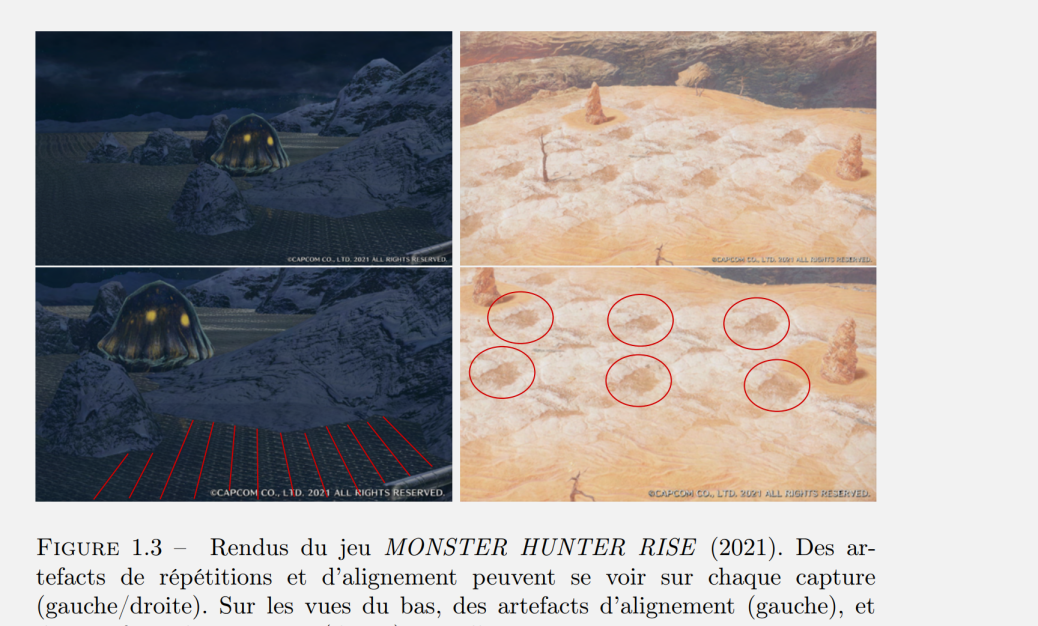
\includegraphics[width=\textwidth]{contenu/resources/images/periodic_tiling}
    \caption[Artefacts d'alignement créés par le pavage périodique]{Artefacts d'alignement créés par le pavage périodique, \textit{Monster Hunter Rise} (2021), Capcom. Crédit à N. Lutz~\cite{lutz_processus_2021} pour l'image.}
    \label{fig:periodic-tiling}
\end{figure}

La gestion de l'équilibre entre cohérence et variété est un enjeu majeur dans la synthèse par réorganisation. La cohérence qualifie comment la synthèse reproduit l'apparence visuelle de l'exemple. La variété est la capacité à générer de la nouveauté dans le contenu généré. L'objectif de la synthèse est de propager une apparence similaire à l'exemple sur une grande surface, comme si l'apparence entière avait été synthétisée directement par un unique procédé. Une bonne synthèse doit ainsi apporter à la fois de la cohérence et de la variété. Le pavage périodique par exemple est très cohérent, mais n'apporte aucune variété. Dans un pavage périodique, la tuile qui est réagencée est en fait la texture entière.

\bigskip

Le faible qualité du pavage périodique illustre l'importance du choix de la taille de tuile dans la gestion de l'équilibre entre cohérence et variété. Une grosse tuile capture bien l'apparence de la texture, mais reproduit des motifs saillants qui causent des artefacts et n'offrent pas beaucoup de variété. À l'inverse avec une petite tuile, seulement quelques texels sont réutilisés et certaines relations entre texels éloignés sont perdues, ce qui cause une perte de cohérence. Il est préférable de prendre des tuiles plus petites et mieux les mélanger~\cite{heitz_high-performance_2018} afin de d'obtenir de la variété et d'éviter la répétition de motifs saillants.


\subsubsection{Synthèse par convolution}

L'objectif d'une synthèse par convolution est de construire une texture en disposant des motifs dits \og noyaux \fg selon une distribution statistique. Un noyau est un petit élément de surface qui peut être un contenu de l'exemple ou du défini de manière fonctionnelle. Le choix du noyau, de la distribution, ainsi que de la méthode de mélange, sont les paramètres à ajuster pour contrôler la synthèse. Une pratique habituelle de la synthèse par convolution est de choisir comme noyau une somme d'ondelettes (typiquement des cosinus) spatialement contraintes et à orientation aléatoire, et de contrôler les fréquences des ondelettes utilisées~\cite{tricard_procedural_2019}. En sélectionnant les fréquences des noyaux, il est possible de contrôler le contenu fréquentiel de la texture synthétisée. Avoir un contrôle sur le contenu fréquentiel de la texture est une bonne méthode pour maîtriser l'apparence de la synthèse~\cite{gilet_local_2014}, comme montré en figure~\ref{fig:lrpn}.

\bigskip

\begin{figure}
    \centering
    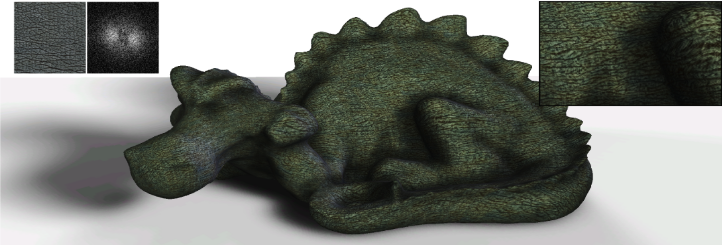
\includegraphics[width=.8\textwidth]{contenu/resources/images/lrpn}
    \caption[Maîtriser le contenu fréquentiel permet de contrôler l'apparence d'une synthèse]{Texture synthétisée par \textit{Local Random Phase Noise}. En approximant le spectre de puissance de l'exemple, Gilet et al.~\cite{gilet_local_2014} ont montré que l'apparence de l'exemple est mieux reproduite.}
    \label{fig:lrpn}
\end{figure}

Cependant, la synthèse de texture comportant de la structure en temps-réel est encore un sujet difficile. Les méthodes existantes de synthèse ne fonctionnent pas lorsque la cible contient des motifs organisés ou de la répétition. Quand des méthodes traditionnelles de synthèse temps-réel sont utilisées sur des textures structurées, des artefacts visuels apparaissent. La figure~\ref{fig:synthesis-failure} montre quelques cas d'échec de synthèses de la littérature appliquées aux textures structurées. Il est difficile de créer du contenu réellement nouveau et préservant le même genre de motifs structurés que ceux de l'exemple, car la synthèse cohérente de structure n'est pas encore possible. Certaines configurations présentant des caractéristiques particulières facilitent le problème. Lutz et al. ont par exemple montré que la synthèse est possible pour des textures dont la structure est régulière~\cite{lutz_cyclostationary-gaussian_2021}. Le cadre général reste néanmoins non résolu.

\begin{figure}
    \centering
    \begin{subfigure}{.45\textwidth}
        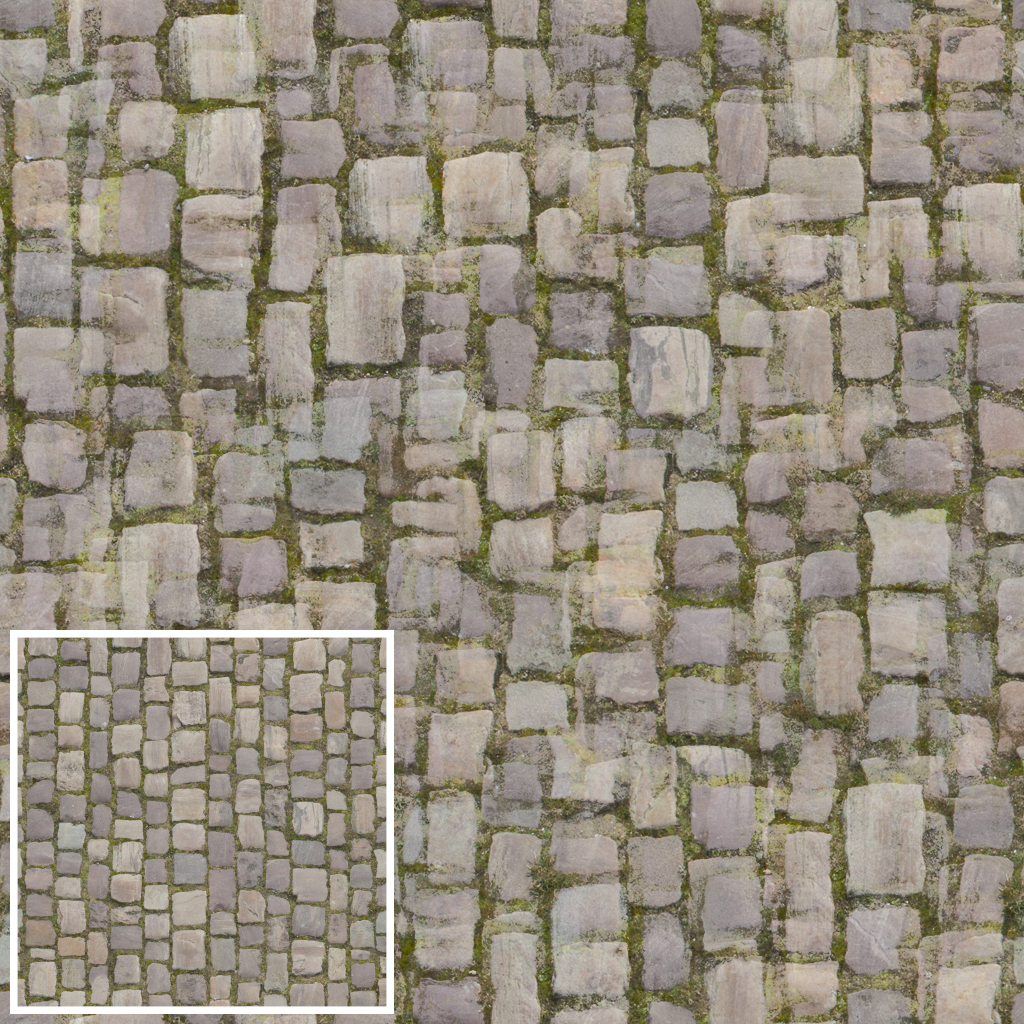
\includegraphics[width=\textwidth]{contenu/resources/images/hpn_failure}
        \caption{Synthèse par pavage et mélange~\cite{heitz_high-performance_2018}.}
    \end{subfigure}
    \hfill
    \begin{subfigure}{.45\textwidth}
        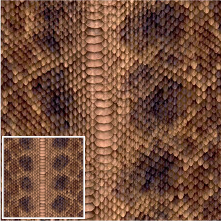
\includegraphics[width=\textwidth]{contenu/resources/images/acf_preserving_hpn_failure}
        \caption{Synthèse préservant la fonction d'autocovariance~\cite{lutz_preserving_2023}.}
    \end{subfigure}

    \caption[Échec de synthèse de texture structurée]{Échec de synthèse de texture structurée. Les méthodes de synthèse actuelles ne sont pas capables de reproduire des textures structurées.}
    \label{fig:synthesis-failure}
\end{figure}

% \section{Génération procédurale} % Non-nécessaire ? De quoi on parle ici sinon ?

% \section{Bruit procédural}

\section{Analyse multi-résolutionnelle locale}

Un enjeu pour synthétiser des textures structurées est de mieux comprendre ce qui compose la structure d'une texture. Pour comprendre la structure d'une texture, l'idée explorée dans cette recherche est d'appliquer des outils de l'analyse d'image à des processus de synthèse. Les outils choisis permettent l'extraction de caractéristiques d'une texture par l'analyse de relations statistiques inter-texels.


Une des raisons pour lesquelles la synthèse de texture contenant de la structure est difficile est qu'il faut préserver certaines relations entre les texels de l'image pour garder la structure. Savoir quelles relations préserver, pour garder la structure de l'image, et quelles relations supprimer, pour ajouter de la variation dans la synthèse, est très délicat, surtout dans le contexte du temps-réel.
% TODO question à soulever plutôt qu'affirmation à faire
% TODO Suggestion : parler de "relations statistiques" plutôt que de "relations", et dire qu'il faut les préserver au mieux. Tu veux préserver toutes les relations statistiques, mais certaines sont trop complexes à préserver en temps réel, en plus d'être difficiles à "capturer". C'est pour ça que tu essayes de développer les outils suivants.
% TODO très délicat = trop vague
% TODO mettre plus bas, après le paragraphe de notion de structure p-e

\subsection*{Notion de structure}

La structure d'une image désigne comment les différentes parties de l'image sont agencées les unes par rapport aux autres, comment les éléments de l'image forment certains schémas ou présentent une certaine forme de régularité. Ces relations sont présentes à différents niveaux d'échelle, on a donc différents niveaux de structure. Savoir quels niveaux préserver et comment est important pour reproduire les caractéristiques désirées de la texture.

\begin{figure}[h!]
    \centering
    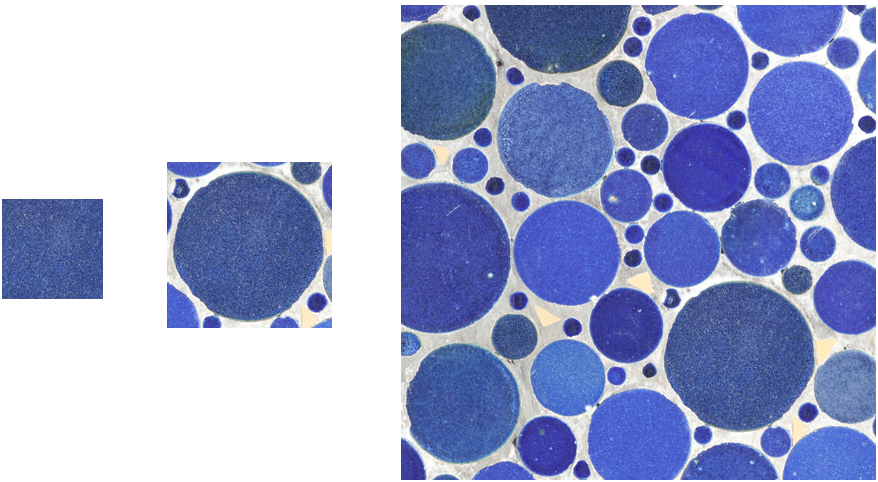
\includegraphics[width=.85\linewidth]{contenu/resources/images/structure_level}
    \caption{Différents niveaux de structure au sein d'une image}
    \label{fig:structure_level}
\end{figure}

\subsection*{Congruence de phases}

Lorsque l'on veut préserver la structure d'une image, les éléments saillants tels que des coins et des lignes, ou plus généralement des bords, sont compliqués à reproduire. On appelle \og bord \fg une région frontière entre un objet et un autre élément de l'image, comme l'arrière plan ou un autre objet. Visuellement, un bord se distingue par un changement brusque de luminosité. Ces changements sont cependant plus difficiles à détecter automatiquement, car le seuil minimum de contraste entre des pixels voisins n'est pas toujours le même, dépendamment de si le bord est franc ou flou. Une approche intéressante est d'utiliser des informations du domaine fréquentiel pour caractériser des bords.
% TODO /!\ luminosité terme nouveau à mieux definir
% p-e image pour illustrer
% TODO "compliqué à reproduire" pourquoi ?
% TODO source pour utilisation domaine fréquentiel

\bigskip

Lorsqu'une image est décomposée dans le domaine de Fourier, on retrouve de nombreuses informations sur la structure dans la phase~\cite{oppenheim_importance_1981}. En explorant le rôle de la phase, Kovesi a mis au point un outil de détection de d'éléments caractéristiques~\cite{kovesi_image_1995} basé sur le modèle physiologiquement réaliste d'énergie locale de Morrone et al.~\cite{morrone_feature_1987, morrone_feature_1988}. Ce modèle postule que les éléments caractéristiques sont présents dans une image là où les composants de Fourier sont maximalement en phase. La congruence de phases qui dérive du modèle d'énergie locale est une grandeur qui quantifie cet alignement. Elle donne lieu à un outil de détection plus robuste que ceux développés auparavant, qui sont souvent sensibles au niveau d'illumination et de grossissement, et nécessitent donc une connaissance a priori des images étudiées. C'est ce modèle de congruence de phases que nous avons repris et adapté à la synthèse de texture.
% TODO paragraphe trop rapide
% étendre et reposer la problématique
% notamment vis a vis de l'aléatoire, préserver congruence avec aléatoire est le noeud du pbl
% todo introduire PC avant de juste en parler

\bigskip

\begin{figure}[h]
    \centering
    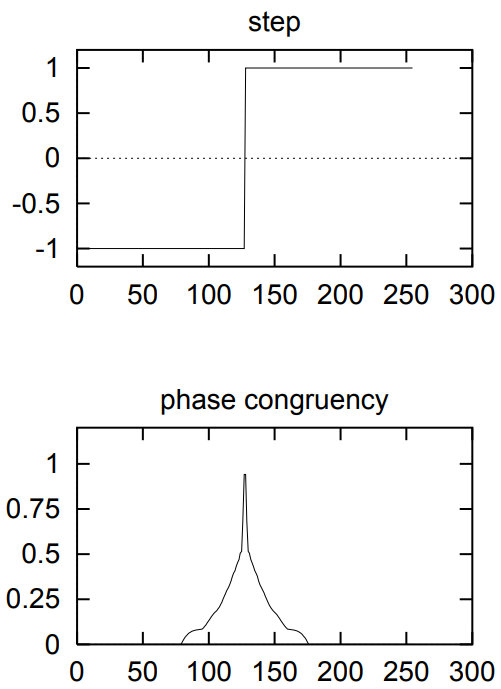
\includegraphics[width=.35\linewidth]{contenu/resources/images/pc_1d_kovesi}
    \caption[Congruence de phases pour un signal 1D]{Congruence de phases pour un signal 1D, Kovesi (1995)~\cite{kovesi_image_1995}}
    \label{fig:pc_1d_kovesi}
\end{figure}

Pour détecter un alignement de phase, il est nécessaire d'avoir un modèle donnant des informations locales sur notre image. Kovesi utilise pour cela une banque de filtres à orientation variable. Nous utilisons à la place le modèle mathématique de la transformée de Riesz, qui permet de décomposer une image dans un espace différent, similairement à la transformée de Fourier, mais avec des informations locales, au niveau du texel (on rappelle que la transformation de Fourier fournit des informations fréquentiellement locales, mais spatialement globales). Utiliser cette transformée nous permet ainsi d'étudier la présence et préservation de relations dans un autre espace que le domaine spatial, donc de mieux comprendre et caractériser nos images.
% TODO dernière ligne : comment pourquoi dans quel but pour atteindre quoi ?

\subsection*{Analyse multi-échelle}

% TODO première phrase : pourquoi ? répond a quel besoin ?
Un objectif de la méthode présentée ici est de pouvoir agir avec précision sur certains niveaux d'échelle de structure ciblés. Une méthode d'analyse qui permet de travailler avec plusieurs niveaux de résolution de la même image est dite \og multi-résolutionnelle \fg~\cite{mallat_theory_1989}, ou multi-échelle. Des exemples d'application communs de méthodes d'analyse multi-résolutionnelle sont la détection robuste de caractéristiques de différentes tailles~\cite{park_multiresolution_2010} et la compression d'images~\cite{averbuch_image_1996}.
%TODO étendre et mieux expliquer. intégrer la phrase d'après qui a été coupée du texte
On décompose notre image en pyramide d'images, ce qui nous permet d'étudier les différences de détails entre les différents niveaux d'échelle.

\section{Plan du manuscript} % / problématique

Ce manuscrit est organisé comme suit :

\begin{itemize}
%    \item revue de l'état de l'art de la synthèse de texture temps réel,
    \item explication de la théorie de Riesz et du modèle d'analyse multi-échelle local qui en découle,
    \item application à la synthèse de texture par échantillonnage préférentiel.
\end{itemize}

	%=========================== CHAPTIRE 0 ============================
	% \modeDefaut  % cette commande s'assure que la langue par défaut est remise si un chapitre est en partie dans une autre langue.
	\modeDefaut
	\chapter{Mise en contexte}
\label{ch:chapitre0}

Ce chapitre fait la mise en contexte du travail présenté dans ce manuscript et introduit les notions nécessaires à la compréhension des chapitres suivants. Les concepts de monde virtuel et ses représentations sont d'abord discutés. Les textures et les méthodes de synthèse, qui sont au cœur de ce travail, sont ensuite abordées. Enfin le principe d'analyse locale multirésolution, utilisé pour étudier la structure des textures, est exposée.

\section{Monde virtuel}

Dans le cadre de l'informatique graphique, un monde virtuel est une méthode de représentation de scènes au moyen d'un support numérique. Une scène est une collection d'objets numériques qui interagissent entre eux. Il existe trois sortes d'objets numériques qui composent une scène : de la géométrie, des lumières et des caméras. Avec des algorithmes de rendu, un monde virtuel peut être converti en image. Les mondes virtuels sont utilisés dans de nombreux domaines~\cite{magnenat-thalmann_introduction_1986}, comme :

\begin{itemize}
    \item le domaine du divertissement, pour les jeux vidéo (l'industrie du jeu-vidéo est un des principaux acteurs des avancées en graphisme) ;
    \item le domaine de l'animation, pour les films d'animation ou les effets spéciaux de films ;
    \item le domaine médical, pour des outils de visualisation de l'anatomie humaine ou de formation en réalité virtuelle ;
    \item le domaine de l'ingénierie, pour aider à la conception d'objets (conception assistée par ordinateur) ou de bâtiments (architecture) ;
    \item le domaine militaire, pour faire des simulations de situations ou des entraînements au combat.
\end{itemize}

\subsection{Types de rendu}

La visualisation de scènes virtuelles s'opérationnalise au travers d'un moteur de rendu utilisant divers algorithmes pour fonctionner~\cite{sherman_chapter_2003}. Un moteur de rendu traite une scène en différentes étapes dans le but d'en créer une visualisation appelée rendu de la scène~\cite{pharr_physically_2023}. Il existe plusieurs méthodes de rendu qui implémentent différents algorithmes pour produire différentes visualisations d'une scène. Pour exécuter leurs calculs, les logiciels de rendu s'appuient sur les capacités des cartes graphiques (\textit{Graphics Processing Unit} ou GPU). Ces dernières sont des processeurs hautement parallèles et spécialisés dès leur fabrication pour des calculs graphiques~\cite{das_history_2016}.

\bigskip

\begin{figure}[t]
    \centering
    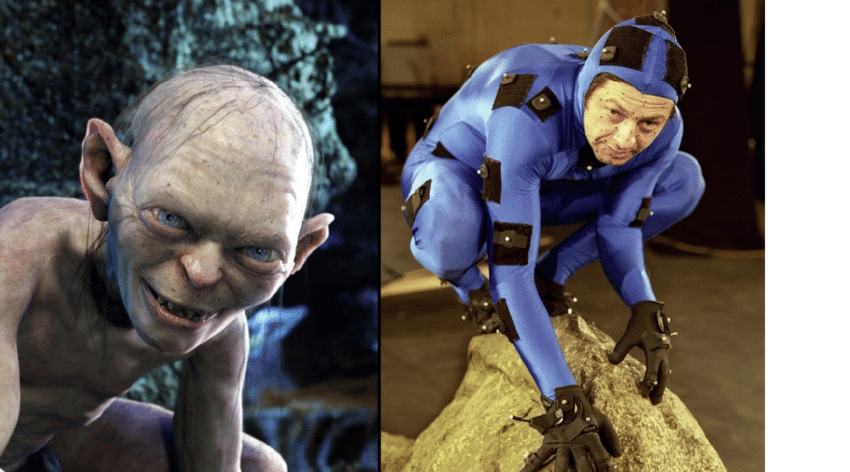
\includegraphics[width=.65\textwidth]{contenu/resources/images/gollum}
    \caption[\textit{Gollum} (2002), \textit{Le Seigneur des Anneaux : Les Deux Tours}]{\textit{Gollum} \protect\footnotemark, personnage complètement généré par image de synthèse par rendu hors-ligne. Image par Mou~\cite{mou_keyframe_2018}.}
    \label{fig:gollum}
\end{figure}

\footnotetext{\textit{The lord of the rings : The two towers}, 2002, Peter Jackson}

Les méthodes de rendu peuvent être séparés en deux grandes catégories : hors-ligne et en temps-réel. Le rendu hors-ligne désigne les algorithmes qui font la visualisation de scènes non interactives, où il n'est pas possible de contrôler les interactions entre les éléments de la scène. Les films d'animation ou les effets spéciaux de films, comme le personnage de Gollum montré en figure~\ref{fig:gollum}, sont des exemples de rendus fait hors-ligne. L'utilisation de méthodes hors-ligne est en fait devenu une norme dans l'industrie cinématographique \footnote{\og The History of CGI in Movies \fg, 2021, Stikky Media, \url{https://www.stikkymedia.com/history-of-cgi-in-movies/}}, car elle permet la création de scènes qu'il serait impossible de tourner à l'aide de caméras traditionnelles. À l'inverse, lors d'un rendu en temps-réel, une personne utilisatrice a un contrôle sur la scène pendant le traitement. Le déplacement d'un personnage dans un jeu-vidéo, la manipulation d'un modèle de pont dans un logiciel d'architecture et l'affichage d'objets dans une application de réalité augmentée sont tous des exemples de contrôles interactifs nécessitant du temps-réel. Une même scène peut être rendue avec différentes méthodes, pour une visualisation finale unique à chaque fois. La figure~\ref{fig:zero-day} montre une scène rendue en temps-réel d'une part et hors-ligne d'autre part. Les enjeux et contextes des rendus hors-ligne et en temps-réel diffèrent. Le travail présenté dans ce manuscrit s'intéresse aux méthodes de rendu en temps-réel. Dans la méthode proposée, bien qu'une partie de préparation des données soit nécessaire, l'image finale est générée en temps-réel. Les problématiques et solutions concernant le rendu hors-ligne ne sont donc pas abordées dans ce travail.

\bigskip

\begin{figure}[ht]
    \centering
    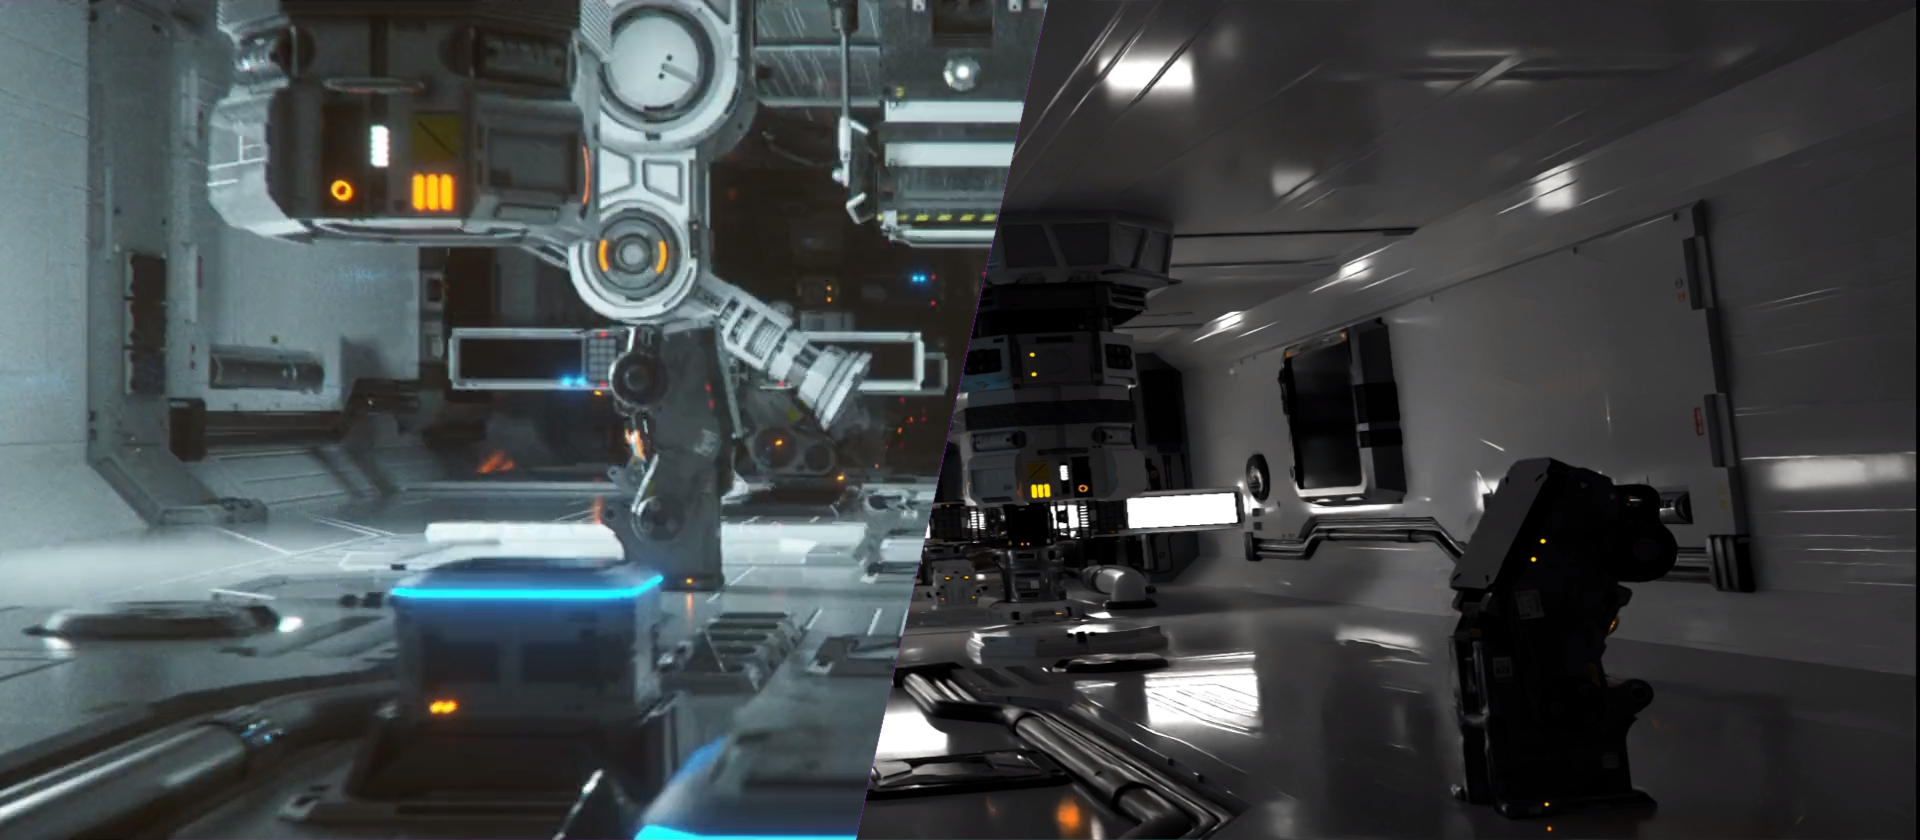
\includegraphics[width=\textwidth]{contenu/resources/images/zero_day_comparison}
    \caption[\textit{Zero-Day} (2015), BEEPLE]{\textit{Zero-Day} (2015), BEEPLE. À gauche rendu original hors-ligne, à droite rendu temps-réel par tracé de chemins, NVIDIA~\cite{winkelman_zero-day_2019}}
    \label{fig:zero-day}
\end{figure}

Une méthode de rendu en temps-réel doit répondre à certaines contraintes dues à la nature interactive de la scène. Le rendu de la scène ne peut pas se faire en avance, car la scène est modifiée pendant l'utilisation. Le rendu doit être assez rapide pour afficher les images de telle sorte que le flux soit continu à l'œil humain. L'industrie cinématographique utilise un standard de 24 images par secondes pour l'enregistrement de films \footnote{\og Why Are Movies 24 FPS - Frame Rate Explained \fg, 2023, Kyle Deguzman, \url{https://www.studiobinder.com/blog/why-are-movies-24-frames-per-second/}}. Pour un rendu en temps-réel, les applications visent des objectifs d'au moins 30 ou 60 images par secondes, afin que le contrôle utilisateur soit confortable~\cite{janzen_is_2014}. Les algorithmes utilisés doivent ainsi être conçus pour s'exécuter avec moins de temps, moins de ressources de calcul, et moins d'espace mémoire disponible.

\subsection{Maillage}

Pour manipuler une scène virtuelle, il est nécessaire d'avoir une représentation des éléments qui la composent. Une représentation est une manière technique de décrire et stocker les données d'une scène. Il y a deux façons de représenter une géométrie dans un monde virtuel. Les représentations continues, comme les surfaces implicites, se rapprochent au mieux des formes des objets du monde réel, mais sont difficiles à créer. Les représentations discrètes, comme les maillages, approximent les représentations continues par des ensembles de polygones~\cite{coons_surfaces_1967}, souvent des triangles. Les polygones qui forment un maillage sont définis explicitement par des données géométriques, notamment les positions des sommets et les sommets des faces. La figure~\ref{fig:procedural-mesh} montre les polygones qui composent un modèle de terrain. Dans ce travail, seuls les maillages seront utilisés. Les maillages sont des structures habituelles dans les mondes virtuels.

\begin{figure}[h]
    \centering
    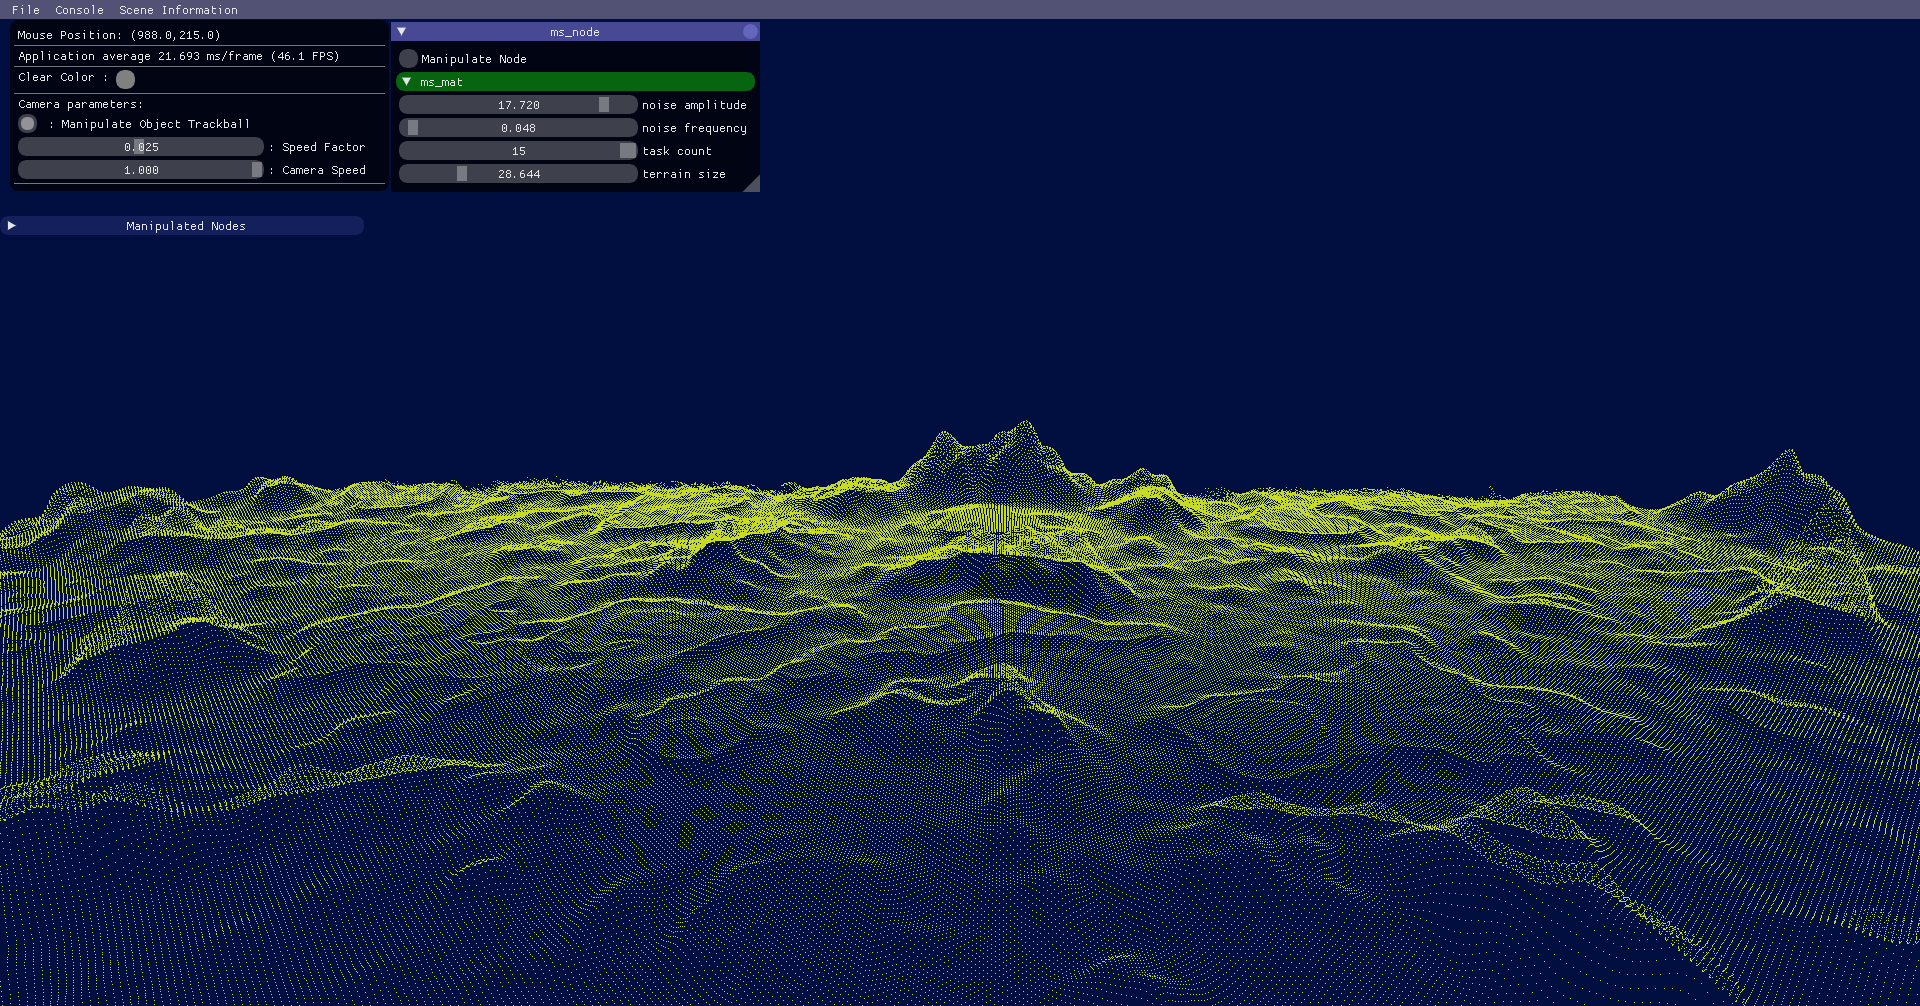
\includegraphics[width=\textwidth]{contenu/resources/images/full_terrain}
    \caption{Maillage d'un terrain généré procéduralement}
    \label{fig:procedural-mesh}
\end{figure}

\section{Texture}

\subsection{Plaquage de texture}

Le maillage utilisé pour représenter une géométrie est une approximation. Pour affiner la géométrie, ou lui attribuer une apparence, il est possible d'utiliser des textures. Une texture est une fonction d'un espace de coordonnées, habituellement à deux ou trois dimensions, à valeurs dans un espace quelconque qui représente les différents attributs possibles de la texture. Les dimensions de l'espace d'arrivée sont appelées canaux de la texture. Les textures représentent généralement la couleur d'une surface, ou d'autres grandeurs physiques comme la profondeur ou l'élévation, qui servent au rendu de la géométrie à laquelle est associée la texture.

\bigskip

\begin{figure}
    \centering
    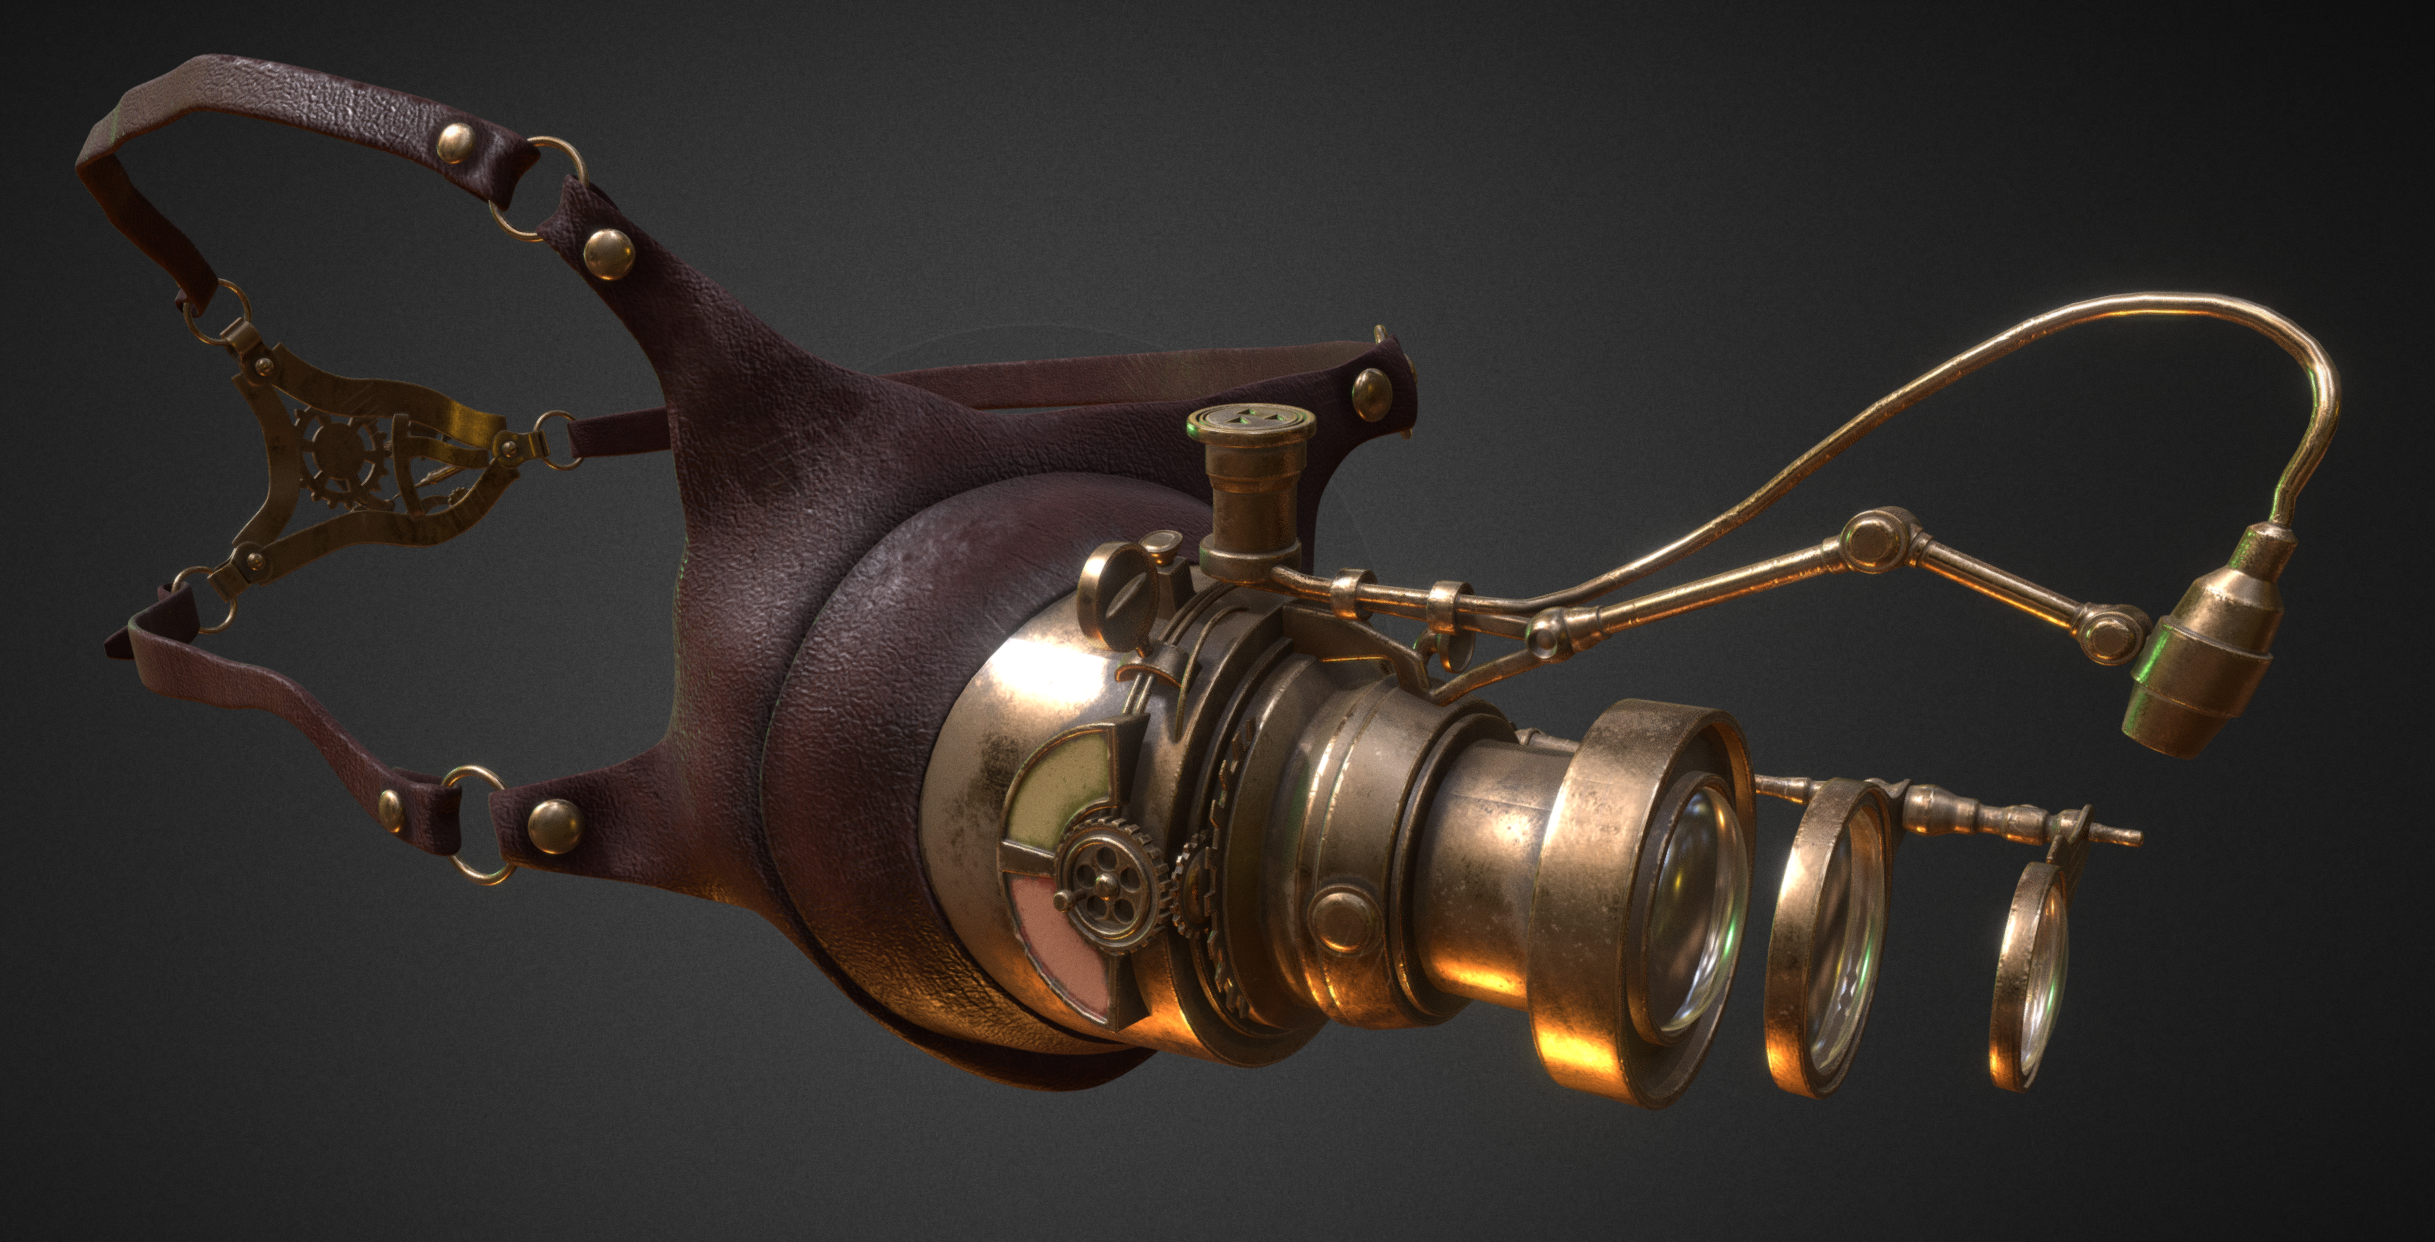
\includegraphics[width=.65\textwidth]{contenu/resources/images/mutli-material-object}
    \caption[Rendu d'un objet comportant plusieurs matériaux]{Plusieurs matériaux différents sont utilisés pour le rendu de cet objet~\cite{lepkarepka_steampunk_2021}}
    \label{fig:multi-material}
\end{figure}

La méthode de travail usuelle en industrie consiste à regrouper ces différentes textures, ainsi que le modèle d'éclairage, dans une ressource dite matériau. Les objets d'une scène sont composés de plusieurs matériaux, qui présentent chacun des propriétés physiques différentes. Dans la figure~\ref{fig:multi-material} par exemple, la lunette a un harnais en cuir, un objectif en métal et des lentilles en verre. Pour créer leurs scènes, les artistes façonnent leurs objets en commençant par la géométrie, avant de créer (ou réutiliser) différents matériaux pour habiller leurs objets.

\bigskip

Il existe deux méthodes classiques de stockage pour une texture : procédurale ou discrète. Une texture procédurale est représenté sous une forme fonctionnelle, à l'aide d'équations ou de procédures. Une texture discrète, quant à elle, est stockée comme une image numérique, c'est-à-dire un tableau discret et fini de données. La représentation procédurale, dont un exemple est donné à la figure~\ref{fig:perlin-noise}, présente plusieurs avantages par rapport à la représentation discrète :

\begin{itemize}
    \item la compacité : pour stocker une texture procédurale, il suffit de stocker les fonctions ou chaines d'instructions qui la définissent. Une texture procédurale n'occupe donc que très peu d'espace en mémoire.
    \item la taille : une texture procédurale est définie comme une fonction sur un espace de paramètre. Une texture procédurale est donc intrinsèquement infinie.
    \item la résolution : une texture procédurale est une fonction continue au sens mathématique. Il est possible de connaître la valeur exacte d'une texture procédurale en n'importe quel point de l'espace de coordonnées en l'évaluant en ce point.
\end{itemize}

Les textures procédurales ont cependant des désavantages. Certaines apparences souhaitées sont difficilement exprimables de manière fonctionnelle. Une expression fonctionnelle peut aussi être difficile à manipuler pour des artistes, puisqu'il faut ajuster des paramètres et modifier l'apparence de manière indirecte. De plus, l'expression d'une texture procédurale est parfois complexe et peut être un enjeu pour la synthèse en temps-réel. Il arrive que la fonction ou suite d'instructions qui définissent une texture procédurale sont si longs à exécuter que le budget de temps pour le rendu de l'image est dépassé. Une texture qui fait dépasser le budget temps du rendu n'est pas viable.

\bigskip

\begin{figure}[t]
    \centering
    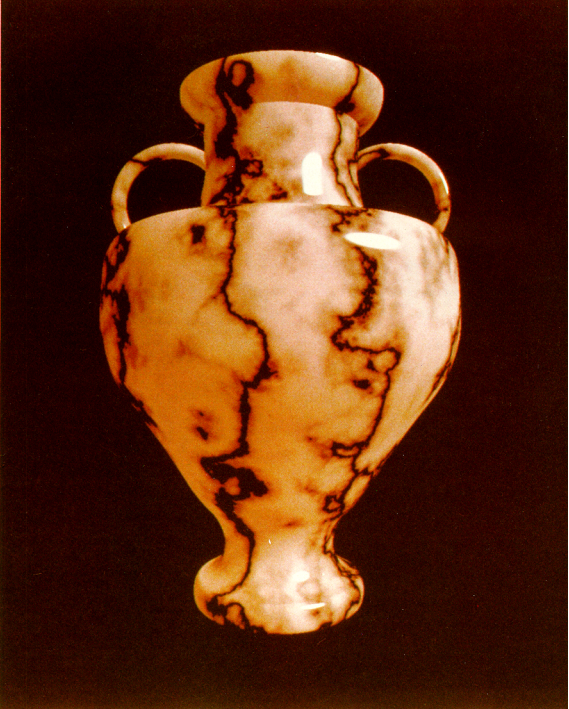
\includegraphics[width=.5\textwidth]{contenu/resources/images/perlin-noise}
    \caption[Bruit de Perlin]{La notion de texture procédurale est introduite par Ken Perlin en 1985 avec son bruit de Perlin~\cite{perlin_image_1985}.}
    \label{fig:perlin-noise}
\end{figure}

Résoudre les problématiques des textures procédurales est un enjeu de l'informatique graphique. Obtenir de nouvelles apparences, avoir un meilleur contrôle par les artistes et une évaluation plus rapide sont des sujets constamment explorés dans le domaine~\cite{heitz_high-performance_2018, tricard_procedural_2019, lutz_cyclostationary-gaussian_2021, baldi_differentiable_2023}. Le sujet présenté dans ce manuscrit s'inscrit dans la problématique de l'agrandissement du champ des apparences représentables par texture procédurale.

\subsection{Échantillonnage}

Le processus utilisé traditionnellement pour le rendu en temps-réel est appelé le pipeline graphique de tramage. Dans ce pipeline, la scène rendue est projetée sur le plan image, qui est une représentation virtuelle de l'écran. La géométrie est ensuite divisée en petits éléments de surface appelés fragments, durant l'étape éponyme de tramage. La figure~\ref{fig:rasterization} montre comment un triangle est tramé dans le pipeline traditionnel. Les fragments sont les éléments atomiques du pipeline : ce sont les plus petits éléments indivisibles manipulés. Au terme du processus de rendu, un fragment est soit défaussé car non visible dans l'image finale, soit donné une couleur et affiché. Un fragment affiché à l'écran est appelé un pixel (mot-valise de \textit{Picture Element}). L'ensemble des pixels forme l'image rendue.

\begin{figure}[t]
    \centering
    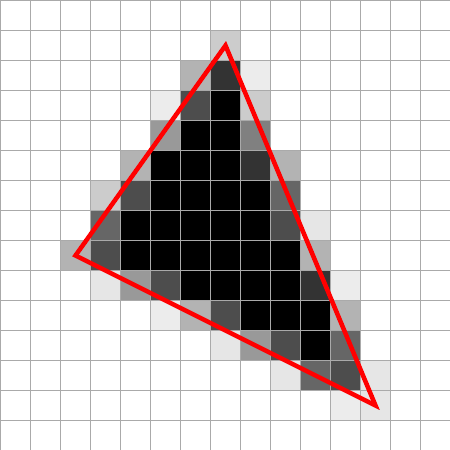
\includegraphics[width=.55\textwidth]{contenu/resources/images/rasterization}
    \caption[Tramage d'un triangle]{Un triangle (rouge) tramé (noir). Crédit à \textit{Wojciech mula} pour l'image.}
    \label{fig:rasterization}
\end{figure}

\bigskip

\begin{figure}
    \centering
    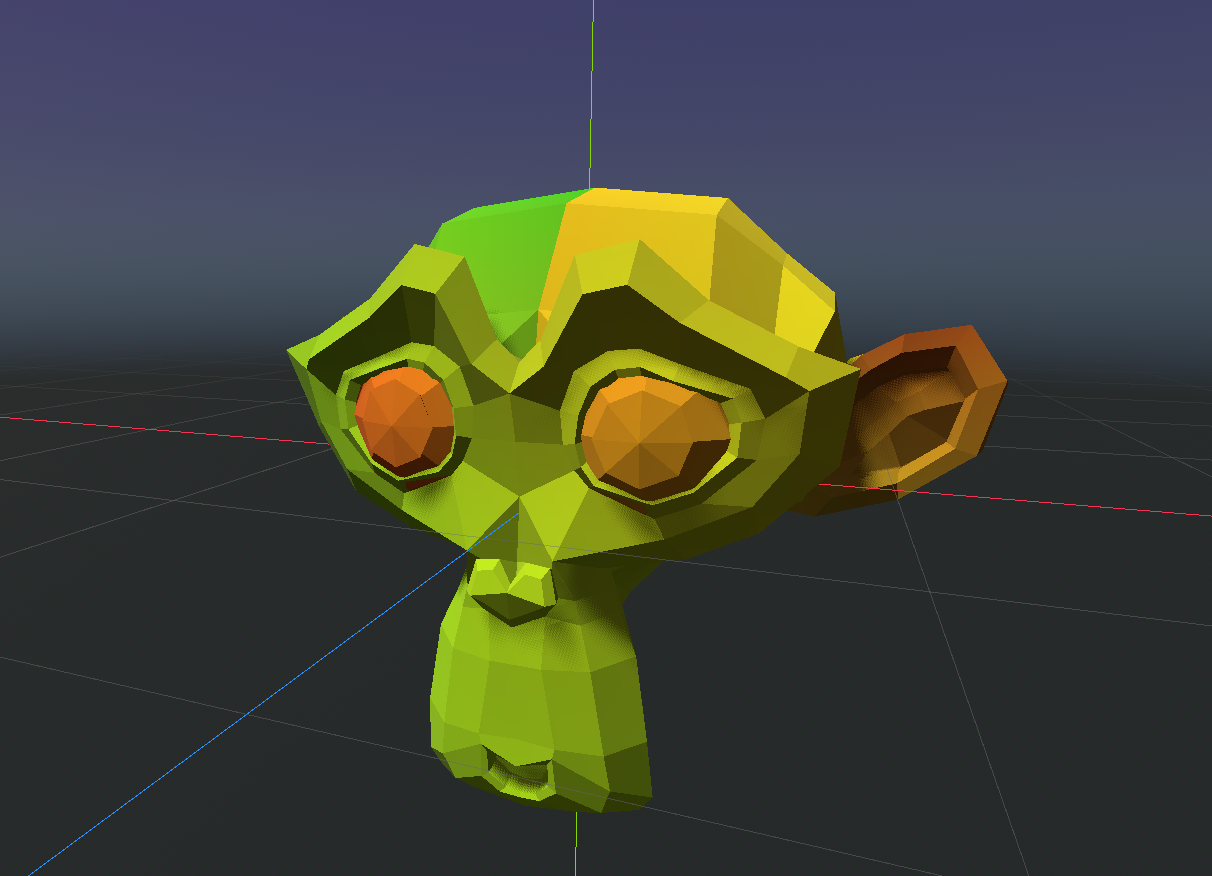
\includegraphics[width=.55\textwidth]{contenu/resources/images/uv_suzanne}
    \caption[Coordonnées UV du modèle Suzanne]{Visualisation des coordonnées UV de Suzanne \footnote{\textit{Suzanne}, 2002, Willem-Paul van Overbruggen}, modèle 3D de référence du logiciel Blender}
    \label{fig:uv-suzanne}
\end{figure}

Pour appliquer une texture à une géométrie, un système de coordonnées UV, est utilisé. Les coordonnées UV sont des vecteurs 2D, entre $(0, 0)$ et $(1, 1)$. Les sommets des maillages des objets de la scène ont chacun des coordonnées UV, qui leurs sont associées à la création de l'objet. Les coordonnées sont ensuite interpolées entre les sommets pour chaque fragment lors du tramage. Un exemple de rendu exhibant les coordonnées UV d'un modèle 3D est montré à la figure~\ref{fig:uv-suzanne}. Les coordonnées UV indiquent quelles parties de la texture correspondent à chaque fragment de la géométrie. L'action d'évaluer une texture en utilisant les coordonnées des fragments est appelée échantillonnage de la texture. Ce processus d'échantillonnage s'effectue en général au moment du rendu.

\subsection{Filtrage}
\label{subsec:filtering}

L'étape d'échantillonnage comporte un problème inhérent, dû au fonctionnement d'un écran et à la nature discrète du système de pixels. Comme expliqué, la géométrie de la scène est projetée, puis découpée en fragments. Le fragment représente donc une partie de surface continue. Mais un fragment est un élément discret, il ne prend qu'une seule valeur. Le schéma en figure~\ref{fig:aliasing} illustre cette problématique. Avec les notations de la figure, un fragment $P$ représente la surface projetée $e(P)$ avec une seule valeur. La valeur que devrait prendre le fragment est l'intégrale de la texture sur l'empreinte $e(P)$. Cette valeur est cependant difficile à calculer dans la majorité des cas. Dans le cas de textures discrètes, une considération supplémentaire doit être faite. L'empreinte du fragment sur la surface texturée est souvent de taille différente que le texel (mot-valise de \textit{Texture Element}) de la texture.

\bigskip

\begin{figure}
    \centering
    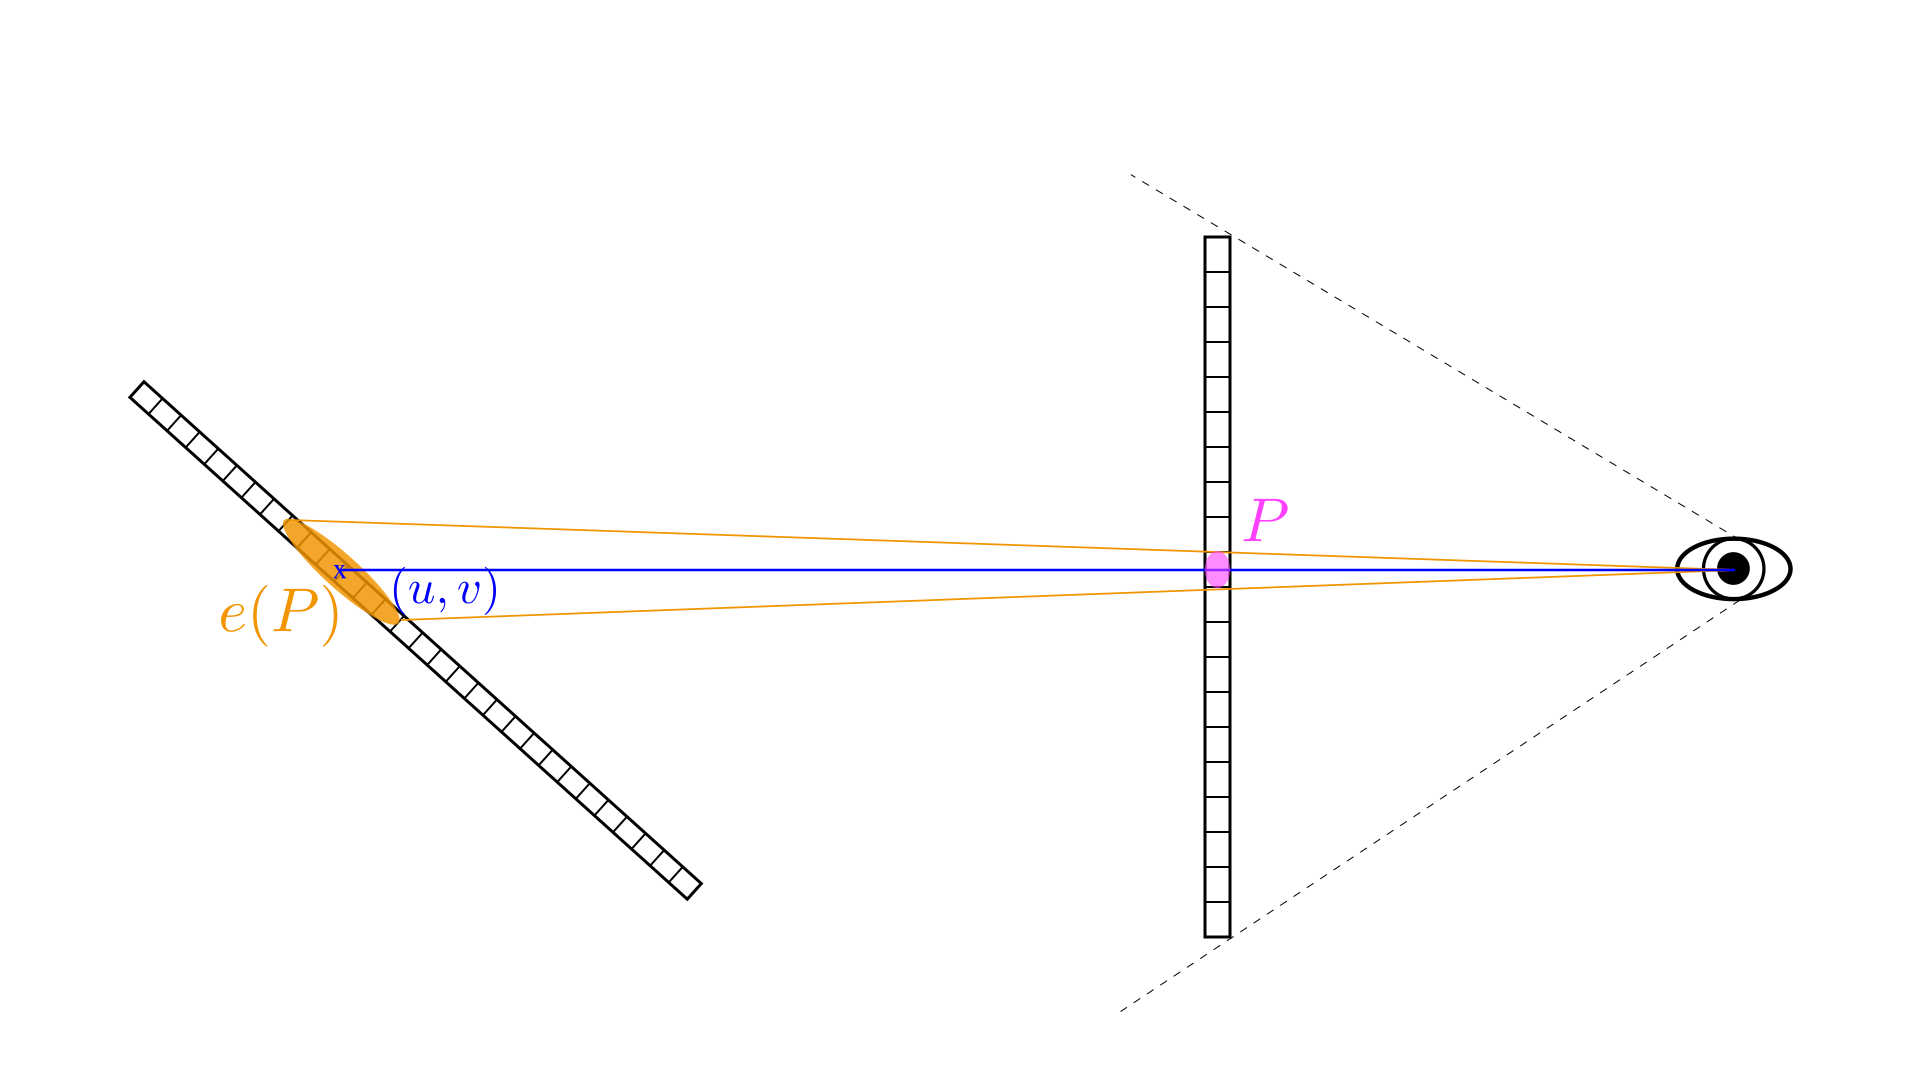
\includegraphics[width=\textwidth]{contenu/resources/images/schema_filtrage}
    \caption[Visualisation du problème d'échantillonnage lors du rendu par tramage]{À cette distance de l'écran, l'empreinte $e(P)$ du fragment sur la surface texturée couvre plusieurs texels. Les coordonnées $(u, v)$ ne sont pas suffisantes pour capturer toute l'information de la texture.}
    \label{fig:aliasing}
\end{figure}

Les comportements indésirables causés lors des étapes de rendu et observables sur l'image finale sont appelés artefacts de visualisation. Dans le cas de l'échantillonnage, les artefacts causés par la différence de taille entre un fragment et son empreinte sur une surface texturée sont appelés artefacts d' aliassage. Pour résoudre les problèmes d'aliassage, plusieurs méthodes dites de filtrage sont utilisées, dépendamment du problème d'aliassage rencontré :

\begin{itemize}
    \item le sur-échantillonnage signifie que l'empreinte d'un fragment est plus petite qu'un texel. En cas de sur-échantillonnage, plusieurs fragments voisins peuvent prendre la même valeur. Avoir une même valeur pour plusieurs fragments voisins donne un aspect crénelé à l'image et les contours des objets sont en escalier. La solution idéale dans ce cas est d'augmenter la résolution de la texture utilisée ; ce n'est cependant pas tout le temps possible. Une alternative commune est de faire l'interpolation des valeurs des quatre texels voisins. La texture est échantillonnée quatre fois pour chaque fragment et l'image prend un aspect légèrement flouté, mais l'effet escalier est réduit. Un exemple est montré à la figure~\ref{fig:filtering}
    \item le sous-échantillonnage indique que l'empreinte d'un fragment est plus grande qu'un texel et en recouvre plusieurs, comme à la figure~\ref{fig:aliasing}. En cas de sous-échantillonnage, des fragments voisins représentent du contenu éloigné spatialement sur la surface. La surface entre les centres des empreintes de fragments voisins est alors mal représentée. De loin, la surface texturée présente des motifs dits de moiré. Des bandes non-présentes dans la texture apparaissent sur le rendu et il y a un effet de scintillement lorsque la caméra est déplacée dans la scène. L'apparence souhaitée est l'intégrale des texels qui sont sous l'empreinte du fragment, mais un algorithme de tramage naïf ne lit qu'un seul texel. La solution idéale serait de calculer l'intégrale sur tous les texels couverts par l'empreinte du fragment. Calculer l'intégrale directement est souvent irréalisable. L'approche traditionnelle dite filtrage tri-linéaire consiste à pré-calculer une approximation de l'intégrale pour différentes tailles d'empreintes et trouver le bon niveau au moment du rendu. Cette approche double l'occupation mémoire pour chaque texture, mais les effets de moiré disparaissent.

%    \item Différentes résolution des textures utilisées appelées MIPs maps sont pré-calculées avant le rendu. Ces MIPs maps sont l'approximation des intégrales de régions de texels de différentes tailles. La technique de filtrage dit tri-linéeaire consiste à trouver les niveaux adéquats de MIPs maps auquel l'empreinte du fragment a une taille similaire à un texel. L'échantillonnage de la texture se fait alors dans les deux niveaux les plus proches.
%    \item L'alternative classique consiste à pré-calculer différentes échelles de la texture utilisée, appelées MIP maps, et de trouver l'échelle adéquate de telle sorte qu'un texel ait la même taille qu'un fragment. L'échantillonnage est plus lourd et on prend plus d'espace mémoire pour stocker les MIP maps, mais la texture est mieux rendue de loin.
\end{itemize}

\bigskip

\begin{figure}
    \centering
    \begin{subfigure}[b]{.45\textwidth}
        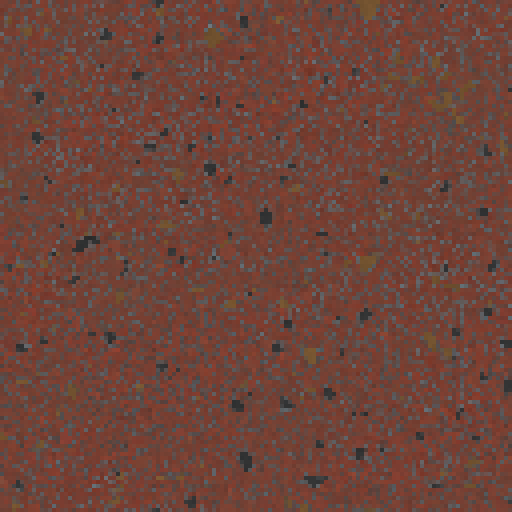
\includegraphics[width=\textwidth]{contenu/resources/images/porcelain_no_filter}
        \caption{Sans filtrage}
    \end{subfigure}
    \hfill
    \begin{subfigure}[b]{.45\textwidth}
        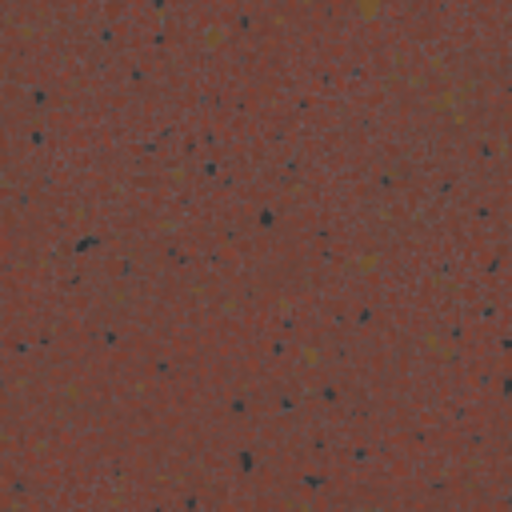
\includegraphics[width=\textwidth]{contenu/resources/images/porcelain_filter}
        \caption{Avec filtrage linéaire}
    \end{subfigure}
    \caption{Filtrer correctement est un enjeu majeur dans l'utilisation des textures}
    \label{fig:filtering}
\end{figure}

S'assurer de filtrer correctement lors de l'échantillonnage est un enjeu majeur pour obtenir un rendu fidèle aux textures utilisées. C'est particulièrement le cas lors la création de textures procédurales, qui est le sujet de cette étude. Diverses méthodes peuvent être utilisées pour la création de textures procédurales. S'assurer de la filtrabilité d'une méthode de création de textures est une des problématiques principales et un critère de qualité de la synthèse de texture, présentée dans la section suivante.

%{\color{red}Pertinence de ce paragraphe ?}
%De nombreuses méthodes de filtrage plus élaborées sont employées pour obtenir des résultats de meilleure qualité, ou pour filtrer des textures plus compliquées. Par exemple quand les textures ne sont plus des images prédéterminées à l'avance, mais qu'elles sont générées au moment du rendu.
% oui pertinent, mentionner les autres solutions "idéales" mais plus difficiles (voir not). filtre analytique et pré-intégration
%OU p-e supprimer paragraphe

\section{Synthèse de texture}

De nombreuses surfaces texturées lors d'un rendu, comme des sols, sont de grande taille. Comme discuté précédemment~\ref{subsec:filtering}, produire des textures de résolution suffisante pour texturer de grandes surfaces sans artefacts demande une grande occupation mémoire et un long temps de création. Étirer les textures en utilisant les coordonnées UV est une solution, qui atteint cependant ses limites assez rapidement. Utiliser une texture de plus basse résolution cause des artefacts visuels. Il est possible de résoudre le problème en créant directement une texture de taille adaptée à la surface à couvrir, procédé appelé synthèse de texture. Par extension, une texture générée par un algorithme de synthèse est aussi appelée une synthèse. Les textures représentent des apparences visuelles de matériaux diverses. Il est possible de classifier des textures de plusieurs manières différentes. Une façon commune de classifier des textures est d'opposer les textures stochastiques, dont les couleurs de pixels semblent aléatoires, et les textures régulières, qui présentent une répétition régulière de motifs~\cite{liu_near-regular_2004}.

\subsection{Notion de structure}
\label{subsec:structure}

Le travail présenté dans ce manuscript s'intéresse cependant à la synthèse de texture présentant de la structure. Le concept de structure, bien que visuellement intuitif, est difficile à définir de manière formelle. Dans le cadre de ce manuscript, la structure d'une texture désigne comment les différentes parties de la structure sont agencées les unes par rapport aux autres. Dans une texture structurée, les éléments de la texture forment certains schémas ou présentent une certaine forme de régularité. La classification de textures utilisée dans ce travail est faite selon le niveau de structure des textures car c'est le thème central de l'étude. La figure~\ref{fig:échelle-structure} illustre la classification proposée.

\bigskip

\begin{figure}
    \centering
    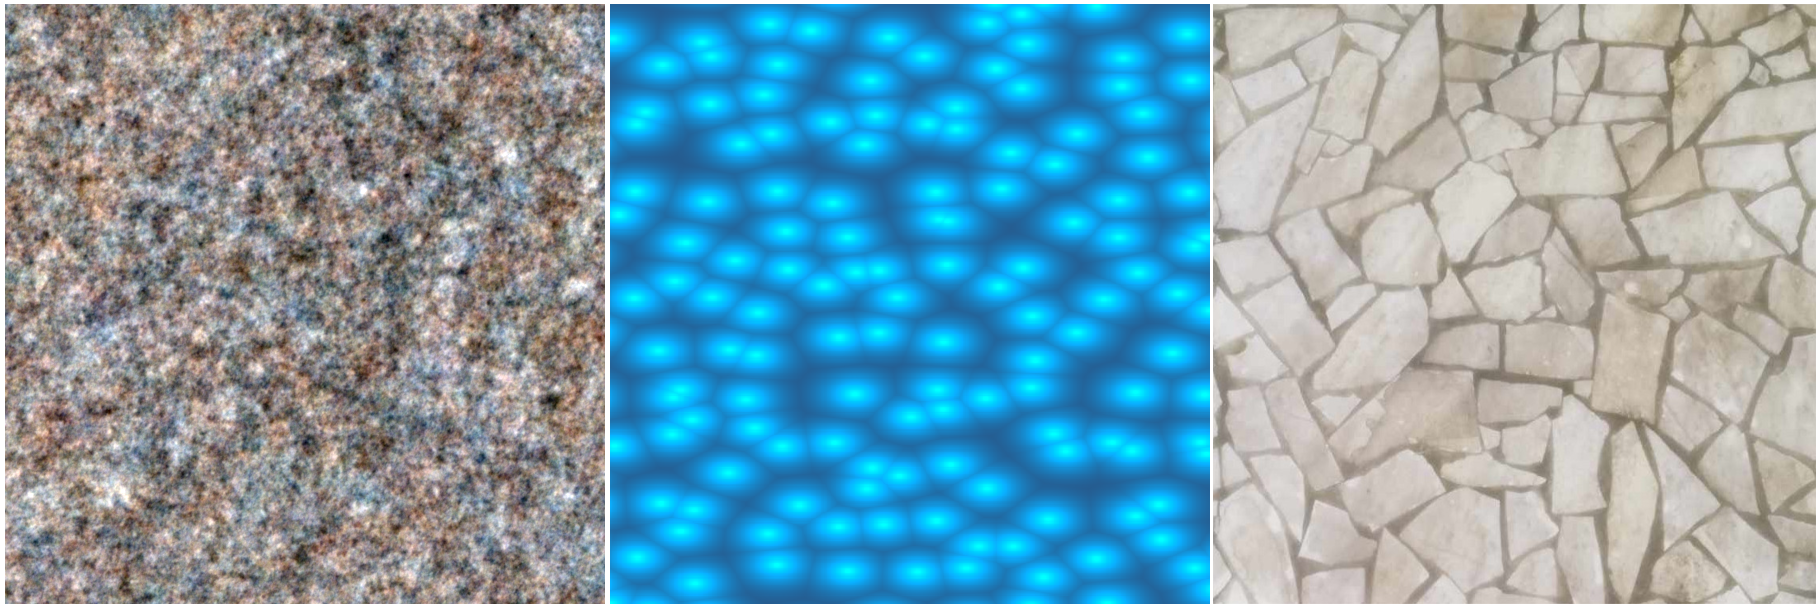
\includegraphics[width=\textwidth]{contenu/resources/images/structure_scale_loucas}
    \caption[Classification des textures selon leur niveau de structure]{Les textures peuvent être classées selon leur niveau de structure : stochastiques ou gaussiennes (gauche), semi-régulières (milieu), ou structurées (droite)}
    \label{fig:échelle-structure}
\end{figure}

L'agencement des éléments de la texture peut se faire à différents niveaux d'échelle. Il y a donc différents niveaux de structure dans une image, principe illustré à la figure~\ref{fig:structure-level}. Les caractéristiques d'une texture telles que l'agencement sont déterminées par des relations statistiques entre les texels de la texture. Préserver toutes les relations statistiques entre les texels est désirable pour la conservation de l'apparence, mais certaines sont trop complexes à préserver en temps-réel. Comprendre quelles relations statistiques préserver et à quel niveau de structure œuvrer sont des enjeux majeurs pour la synthèse de texture structurée et sont l'objet de ce travail.

\begin{figure}
    \centering
    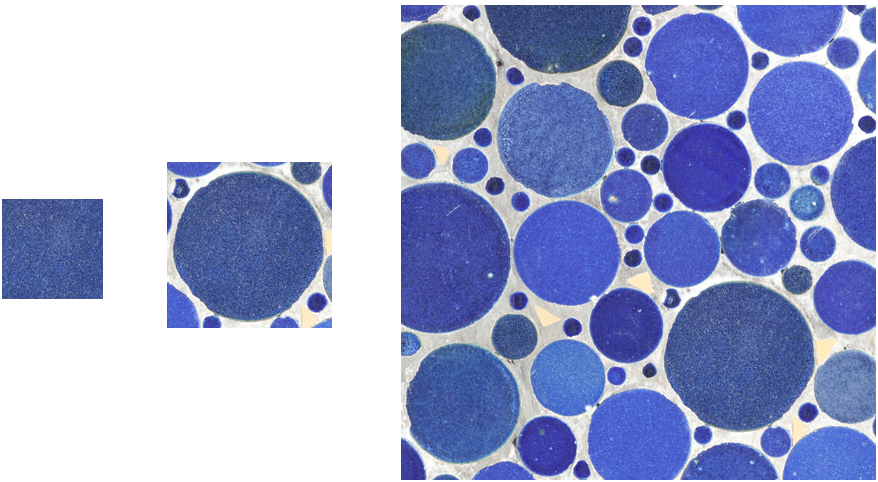
\includegraphics[width=.85\linewidth]{contenu/resources/images/structure_level}
    \caption{Différents niveaux de structure au sein d'une image}
    \label{fig:structure-level}
\end{figure}

\subsection{Algorithme de synthèse}

Une synthèse de texture un procédé qui permet de produire une texture de taille arbitraire, pouvant prendre en argument des paramètres de différente nature. Différentes synthèses possèdent différentes propriétés, qui peuvent être voulues ou non en fonction de la scène à rendre. Par exemple la texture générée est souvent infinie, il est possible de l'appliquer à des surfaces de taille quelconque avec la résolution désirée. De plus, la texture est évaluée au vol (pendant le rendu) et n'a pas besoin d'être stockée en mémoire. Cela réduit l'occupation mémoire de la texture.

\bigskip

Il existe plusieurs types de synthèses différentes, qui produisent des types de textures différentes. Une première distinction majeure qui est souvent faite est, comme pour le rendu, entre une synthèse hors-ligne et une synthèse en temps réel. Les ressources en temps et en puissance de calcul impliquées diffèrent, les enjeux ne sont pas les mêmes. Les travaux proposés étudient le rendu et la synthèse temps-réel, les synthèses hors-lignes comme les synthèses par optimisation ou par apprentissage profond ne seront pas abordées. Les algorithmes étudiés ici ont la contrainte de devoir s'exécuter au vol, sans que le budget de temps du rendu dépasse le seuil établi. Pour rentrer dans ces contraintes de temps, les méthodes de synthèse exploitent la puissance des cartes graphiques, notamment leur aspect hautement parallélisable. Les algorithmes de synthèse doivent s'exécuter de manière parallèle et chaque fragment doit se calculer indépendamment de ses voisins.

\subsection{Synthèse temps-réel} % / Types de synthèse

Sous ces contraintes d'efficacité et de rapidité, de nombreux algorithmes subsistent ; deux grandes catégories de méthodes courantes sont la synthèse par réorganisation et la synthèse par convolution.

\subsubsection{Synthèse par réorganisation}

Le but d'une synthèse par réorganisation est de reproduire un extrait de texture donné en entrée en réutilisant et réagençant son contenu. Dans une synthèse par réorganisation, le contenu est découpé en petites régions connexes dites « tuiles ». Plusieurs paramètres comme la taille, forme et disposition des tuiles peuvent être modifiés pour varier la synthèse. L'exemple le plus simple de synthèse par réorganisation est le pavage périodique. Dans un pavage périodique, la texture d'entrée est simplement répétée jusqu'à couvrir la surface désirée. Pour pouvoir faire un pavage périodique, il faut que la texture d'entrée soit périodique, c'est-à-dire qu'elle se répète sans coupure. Le pavage périodique, bien que très rapide, est de faible qualité. Des artefacts visuels sont induits, car il n'y a aucune variation au sein de la texture générée et les motifs sont répétés très régulièrement. Quelques exemples d'artefacts visuels causés par un pavage périodique sont montrés à la figure~\ref{fig:periodic-tiling}. Certains motifs dits saillants sont particulièrement visibles et attirent l'œil, à cause de leur couleur ou de leur forme par exemple. La répétition régulière de motifs saillants n'existe en général pas dans la nature, elle attire encore plus le regard d'une personne observatrice et réduit la sensation d'immersion dans la scène.

\bigskip

\begin{figure}
    \centering
    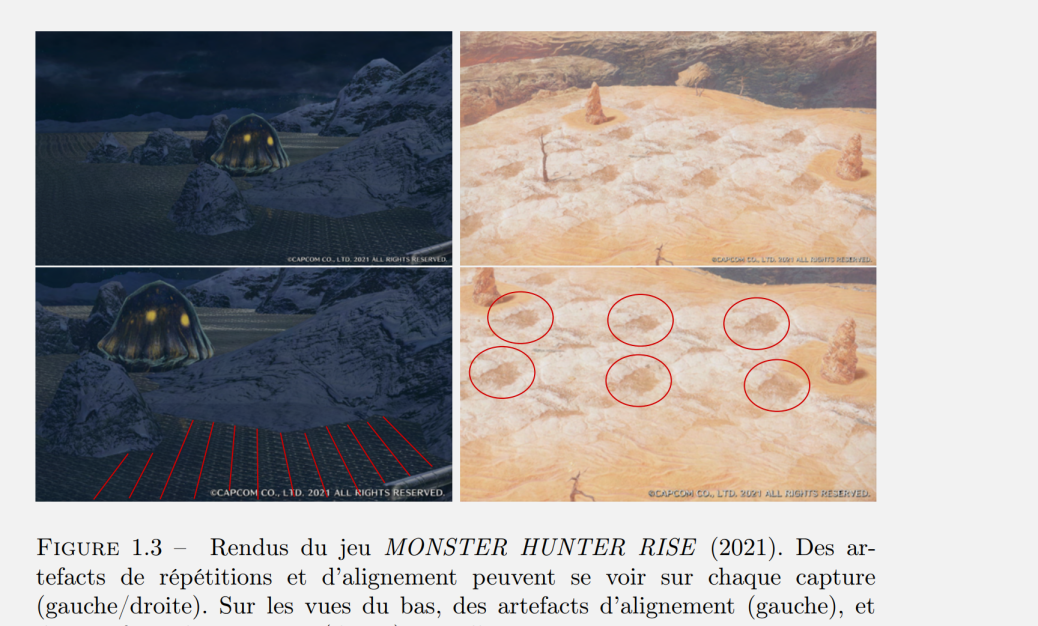
\includegraphics[width=\textwidth]{contenu/resources/images/periodic_tiling}
    \caption[Artefacts d'alignement créés par le pavage périodique]{Artefacts d'alignement créés par le pavage périodique, \textit{Monster Hunter Rise} (2021), Capcom. Crédit à \textit{Nicolas Lutz}~\cite{lutz_processus_2021} pour l'image.}
    \label{fig:periodic-tiling}
\end{figure}

La gestion de l'équilibre entre cohérence et variété est un enjeu majeur dans la synthèse par réorganisation. La cohérence qualifie comment la synthèse reproduit l'apparence visuelle de l'exemple. La variété est la capacité à générer de la nouveauté dans le contenu généré. L'objectif de la synthèse est de propager une apparence similaire à l'exemple sur une grande surface, comme si l'apparence entière avait été synthétisée directement par un unique procédé. Une bonne synthèse doit ainsi apporter à la fois de la cohérence et de la variété. Le pavage périodique par exemple est très cohérent, mais n'apporte aucune variété. Dans un pavage périodique, la tuile qui est réagencée est en fait la texture entière.

\bigskip

Le faible qualité du pavage périodique illustre l'importance du choix de la taille de tuile dans la gestion de l'équilibre entre cohérence et variété. Une grosse tuile capture bien l'apparence de la texture, mais reproduit des motifs saillants qui causent des artefacts et n'offrent pas beaucoup de variété. À l'inverse avec une petite tuile, seulement quelques texels sont réutilisés et certaines relations entre texels éloignés sont perdues, ce qui cause une perte de cohérence. Il est préférable de prendre des tuiles plus petites et mieux les mélanger~\cite{heitz_high-performance_2018} afin de d'obtenir de la variété et d'éviter la répétition de motifs saillants.


\subsubsection{Synthèse par convolution}

L'objectif d'une synthèse par convolution est de construire une texture en disposant des motifs dits noyaux selon une distribution statistique. Un noyau est un petit élément de surface qui peut être un contenu de l'exemple ou du défini de manière fonctionnelle. Le choix du noyau, de la distribution, ainsi que de la méthode de mélange, sont les paramètres à ajuster pour contrôler la synthèse. Une pratique habituelle de la synthèse par convolution est de choisir comme noyau une somme d'ondelettes (typiquement des cosinus) spatialement contraintes et à orientation aléatoire, et de contrôler les fréquences des ondelettes utilisées~\cite{tricard_procedural_2019}. En sélectionnant les fréquences des noyaux, il est possible de contrôler le contenu fréquentiel de la texture synthétisée. Avoir un contrôle sur le contenu fréquentiel de la texture est une bonne méthode pour maîtriser l'apparence de la synthèse~\cite{gilet_local_2014}, comme montré en figure~\ref{fig:lrpn}.

\bigskip

\begin{figure}
    \centering
    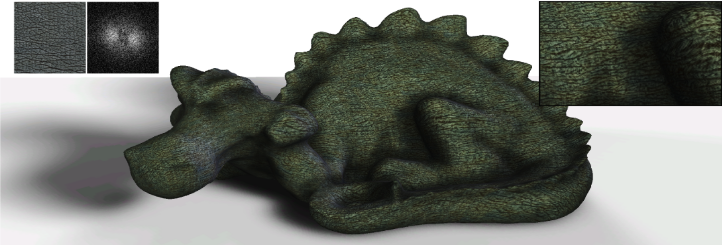
\includegraphics[width=.8\textwidth]{contenu/resources/images/lrpn}
    \caption[Maîtriser le contenu fréquentiel permet de contrôler l'apparence d'une synthèse]{Texture synthétisée par \textit{Local Random Phase Noise}. En approximant le spectre de puissance de l'exemple, Gilet \textit{et al.}~\cite{gilet_local_2014} ont montré que l'apparence de l'exemple est mieux reproduite.}
    \label{fig:lrpn}
\end{figure}

Cependant, la synthèse de texture comportant de la structure en temps-réel est encore un sujet difficile. Les méthodes existantes de synthèse ne fonctionnent pas lorsque la cible contient des motifs organisés ou de la répétition. Quand des méthodes traditionnelles de synthèse temps-réel sont utilisées sur des textures structurées, des artefacts visuels apparaissent. La figure~\ref{fig:synthesis-failure} montre quelques cas d'échec de synthèses de la littérature appliquées aux textures structurées. Il est difficile de créer du contenu réellement nouveau et préservant le même genre de motifs structurés que ceux de l'exemple, car la synthèse cohérente de structure n'est pas encore possible. Certaines configurations présentant des caractéristiques particulières facilitent le problème. Lutz \textit{et al.} ont par exemple montré que la synthèse est possible pour des textures dont la structure est régulière~\cite{lutz_cyclostationary-gaussian_2021}. Le cadre général reste néanmoins non résolu.

\begin{figure}
    \centering
    \begin{subfigure}{.45\textwidth}
        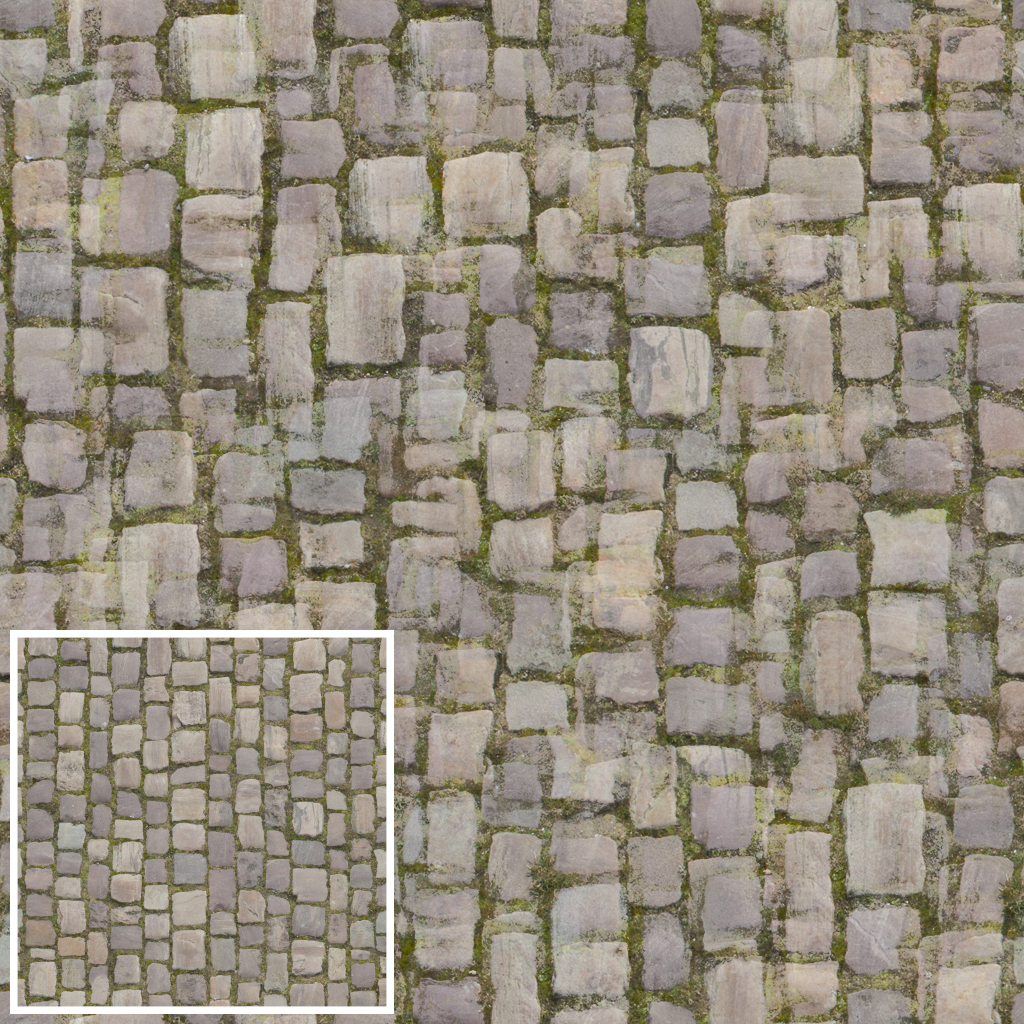
\includegraphics[width=\textwidth]{contenu/resources/images/hpn_failure}
        \caption{Synthèse par pavage et mélange~\cite{heitz_high-performance_2018}.}
    \end{subfigure}
    \hfill
    \begin{subfigure}{.45\textwidth}
        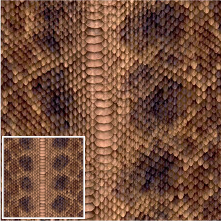
\includegraphics[width=\textwidth]{contenu/resources/images/acf_preserving_hpn_failure}
        \caption{Synthèse préservant la fonction d'autocovariance~\cite{lutz_preserving_2023}.}
    \end{subfigure}

    \caption[Échec de synthèse de texture structurée]{Échec de synthèse de texture structurée. Les méthodes de synthèse actuelles ne sont pas capables de reproduire des textures structurées.}
    \label{fig:synthesis-failure}
\end{figure}

\section{Analyse locale multirésolution}

Un enjeu pour synthétiser des textures structurées est de mieux comprendre ce qui compose la structure d'une texture. Pour comprendre la structure d'une texture, l'idée explorée dans cette recherche est d'appliquer des outils de l'analyse d'image à des processus de synthèse. Les outils choisis permettent l'extraction de caractéristiques d'une texture par l'analyse de relations statistiques inter-texels.

\subsection{Congruence de phases}

Dans une image, une discontinuité de luminosité est appelée un bord~\cite{torre_edge_1986}. La luminosité ou intensité lumineuse mesure la capacité d'une surface à éclairer dans une certaine direction. En informatique graphique, la luminosité désigne une quantité de lumière présente dans une image. Il a été observé qu'une discontinuité dans la luminosité correspond fréquemment à une discontinuité de la profondeur, de l'orientation, de la reflectance ou de la luminance~\cite{lindeberg_edge_1998}. Les bords d'une image sont donc en lien avec les caractéristiques physiques de la scène représentée. Les bords peuvent représenter une région frontière entre un objet et un autre élément de l'image, comme l'arrière-plan ou un autre objet.

\bigskip

\begin{figure}[t]
    \centering
    \begin{subfigure}[b]{.45\textwidth}
        \centering
        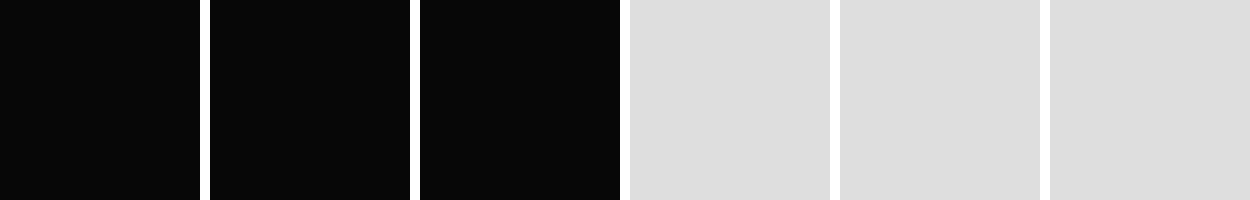
\includegraphics[width=\textwidth]{contenu/resources/images/discrete_discontinuity}
        \caption{Bord franc}
    \end{subfigure}
    \\
    \vspace{1em}
    \begin{subfigure}[b]{.45\textwidth}
        \centering
        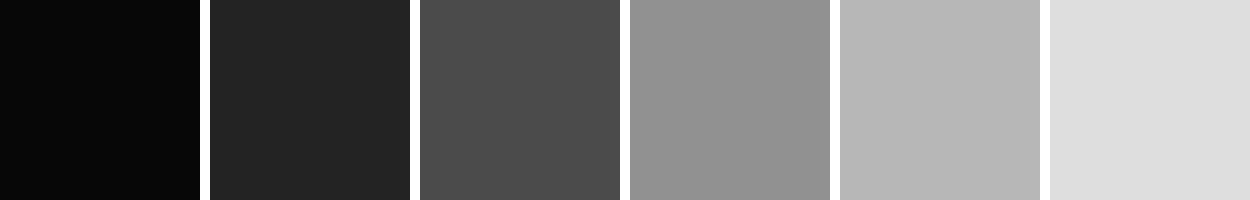
\includegraphics[width=\textwidth]{contenu/resources/images/discrete_smooth}
        \caption{Bord doux}
    \end{subfigure}
    \caption[Difficulté à définir un bord]{Ces signaux 1D discrets ont des discontinuités en luminosité et représentent un bord. Le premier signal (en haut) a une discontinuité franche, le second (en bas) a une discontinuité floues.}
    \label{fig:edge-difficulty}
\end{figure}

Les bords font partie des éléments qui composent la structure d'une image. Préserver la structure implique donc de préserver les bords. La détection de bords est une tâche difficile car le niveau de discontinuité entre deux texels représentant un bord n'est pas fixé, comme illustré à la figure~\ref{fig:edge-difficulty}. Afin de caractériser les bords et comprendre comment les préserver, il est possible d'utiliser des informations du domaine fréquentiel.

\bigskip

Une image peut être exprimée dans le domaine fréquentiel, ou de Fourier, à l'aide de la transformée de Fourier. Contrairement à la représentation par des texels, dit domaine spatial, l'expression dans le domaine fréquentiel permet de séparer les composantes de l'image selon leur fréquence. La transformée de Fourier est une transformation linéaire qui permet de passer d'une représentation à l'autre. La représentation d'une image dans le domaine de Fourier est dite représentation fréquentielle. Une décomposition dans le domaine fréquentiel permet d'extraire de l'information sur des caractéristiques de l'image qui ne sont pas visibles dans le domaine spatial \footnote{\og Fourier transform of images \fg, P. Strumillo et M. Strzelecki, \url{http://mstrzel.eletel.p.lodz.pl/mstrzel/pattern_rec/fft_ang.pdf}}. En particulier Oppenheim a montré que des informations sur la structure d'une image se trouvent dans la phase de sa représentation fréquentielle~\cite{oppenheim_importance_1981}. Morrone \textit{et al.} ont mis au point un modèle physiologiquement réaliste d'énergie locale~\cite{morrone_feature_1987, morrone_feature_1988} qui permet d'extraire des informations sur les éléments saillants d'une image en utilisant la phase. Leur modèle postule que les éléments caractéristiques sont présents dans une image là où les composants de Fourier sont maximalement en phase. Morrone \textit{et al.} introduisent la congruence de phases, grandeur qui quantifie l'alignement de phase des composants de Fourier.

\bigskip

\begin{figure}[t]
    \centering
    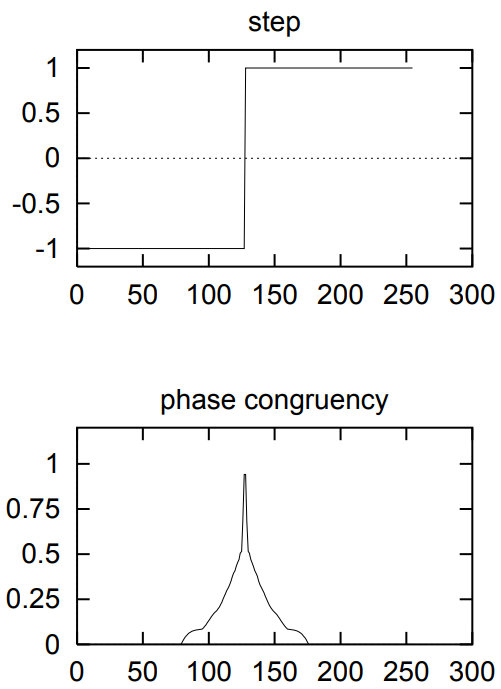
\includegraphics[width=.35\linewidth]{contenu/resources/images/pc_1d_kovesi}
    \caption[Congruence de phases pour un signal 1D]{Congruence de phases pour un signal 1D, Kovesi (1995)~\cite{kovesi_image_1995}}
    \label{fig:pc-1D-kovesi}
\end{figure}

Le travail présenté dans ce manuscript s'intéresse à la congruence de phases comme un moyen d'aider la création de nouvelle structure lors de la synthèse d'une texture. L'objectif est de créer de la structure en introduisant de l'aléatoire, mais de contrôler le processus à l'aide de la congruence de phases. L'étude s'appuie sur les travaux de Kovesi~\cite{kovesi_image_1995}, qui a étendu le modèle de Morrone \textit{et al.}~\cite{morrone_feature_1987, morrone_feature_1988} pour extraire de l'information locale des images~\ref{fig:pc-1D-kovesi}. Une des limites de la transformée de Fourier est en effet que l'information obtenue est spatialement globale. La représentation fréquentielle d'une image ne donne pas directement d'informations sur les relations locales entre les texels. C'est le modèle de Kovesi qui est repris et modifié dans ce travail pour extraire de l'information locale des images. Le modèle de Kovesi est redéfini à l'aide d'un outil mathématique appelé trasnformée de Riesz. La transformée de Riesz permet une représentation alternative d'un signal, avec des informations locales. L'image est ré-exprimée dans un espace différent qui facilite l'étude des relations locales entre les texels.

\subsection{Analyse multi-échelle}

Comme expliqué précédemment, la structure d'une image est composée de plusieurs niveaux d'échelle. Le travail décrit dans ce manuscrit a pour objectif de synthétiser de la nouvelle structure en préservant certains niveaux de structure et en ajoutant de l'aléatoire à d'autres. Un but de la méthode présentée ici est de pouvoir agir avec précision sur certains niveaux d'échelle de structure ciblés. Une méthode d'analyse qui permet de travailler avec plusieurs niveaux de résolution d'une même image est dite multirésolution~\cite{mallat_theory_1989}, ou multi-échelle. Des exemples d'application communs de méthodes d'analyse multirésolution sont la détection robuste de caractéristiques de différentes tailles~\cite{park_multiresolution_2010} et la compression d'images~\cite{averbuch_image_1996}. Dans cette étude, l'analyse multirésolution est faite à l'aide d'une pyramide d'images. Une pyramide d'images est une méthode de représentation d'image qui permet d'étudier les différences de détails entre les différents niveaux d'échelle.

	%=========================== CHAPTIRE 1 ============================

	\modeDefaut
	\chapter[Modèle de Riesz]{Étude théorique du modèle de Riesz} % signal monogénique ?
\label{chap:chapitre1}

Dans le but de synthétiser du contenu avec de la structure irrégulière, une approche locale est adoptée. Ce travail utilise le modèle du signal monogène~\cite{felsberg_monogenic_2001}, qui permet d'extraire l'énergie locale, en s'appuyant sur la transformée de Riesz. Le signal monogène est ensuite mis en application dans un cadre multirésolution, en utilisant une pyramide de Riesz~\cite{wadhwa_riesz_2014} pour calculer la congruence de phases.

\section{Signal monogène}

Le signal monogène est un outil du domaine du traitement du signal introduit par Felsberg et Sommer~\cite{felsberg_monogenic_2001}. Le signal monogène est utilisé pour des tâches d'analyse d'image ou de vision par ordinateur, comme la détection de caractéristiques. La revue de la méthode par Bridge~\cite{bridge_introduction_2018} est une introduction simple et compréhensive aux principes théoriques du signal monogène. Le travail de Bridge est repris dans cette partie, ainsi que ses notations et son discours, afin de prodiguer une compréhension du modèle.

\subsection{Une dimension, signal analytique}

\subsubsection{Construction du signal analytique}

Pour comprendre l'utilité du signal monogène, il faut expliquer le fonctionnement du signal analytique. Le signal monogène est ensuite défini comme l'extension du signal analytique aux signaux de dimension arbitraire. Le signal analytique est une méthode de représentation d'un signal 1D à valeurs réelles, qui facilite la manipulation et l'extraction de certaines informations du signal original. Le constat qui donne lieu à cette représentation est que pour un signal à valeurs réelles, les fréquences négatives sont superflues pour sa représentation de Fourier. En effet, la transformée de Fourier $F(\omega)$ d'un signal à valeurs réelles $f(t)$ présente une symétrie hermitienne :

\begin{equation}
    F(-\omega) = \overline{F(\omega)}
\end{equation}

avec $\overline{\cdot}$ l'opérateur de conjugaison complexe. Les fréquences négatives, non-nécessaires, peuvent donc être mises de côté sans perte d'information. Un nouveau signal est construit en n'utilisant que les fréquences positives de $f(t)$. Le signal $F_{\alpha}$ est d'abord exprimé dans le domaine de Fourier :

\begin{equation}
    F_{\alpha}(\omega) = \left\{
    \begin{array}{ll}
        2F(\omega), & \omega > 0 \\
        0, & \omega < 0 \\
        F(0), & \omega = 0,
    \end{array}
    \right.
\end{equation}

où l'amplitude des composantes de fréquences positives est doublée, par soucis de conservation d'énergie. Avec cette formulation, toute l'information du signal original est conservée. Cette nouvelle forme permet en plus de faire des manipulations précédemment impossibles, qui permettent de mieux comprendre le signal.

\begin{figure}[h]
    %\noindent
    \hspace{-12pt}
    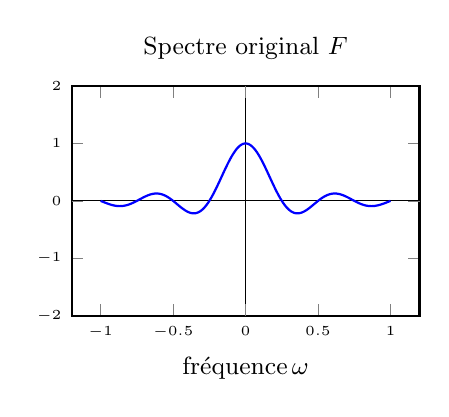
\begin{tikzpicture}
    \begin{axis}[
        title={Spectre original $F$},
        title style={font=\small},
        axis lines=box,
        style=thick,
        xlabel=\(\textnormal{fréquence}\, \omega\),
        xtick={-1, -0.5, 0.5, 1},
        ytick={-2, -1, 1, 2},
        extra x ticks=0,
        extra y ticks=0,
        extra x tick style={grid=major, grid style={black}},
        extra y tick style={grid=major, grid style={black}},
        tick label style={font=\tiny},
        label style={font=\small},
        ymin=-2, 
        ymax=2,
        ]
    \addplot[
        color=blue,
        domain=-1:1,
        samples=200
        ]
    {sin(360*x*2)/ (2*pi*x*2)};
    \end{axis}
    \end{tikzpicture}
    %\hskip 6pt
    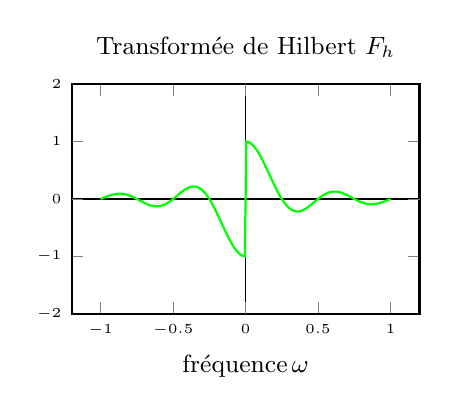
\begin{tikzpicture}
    \begin{axis}[
        title={Transformée de Hilbert $F_h$},
        title style={font=\small},
        axis lines=box,
        style=thick,
        xlabel=\(\textnormal{fréquence}\, \omega\),
        xtick={-1, -0.5, 0.5, 1},
        ytick={-2, -1, 1, 2},
        extra x ticks=0,
        extra y ticks=0,
        extra x tick style={grid=major, grid style={black}},
        extra y tick style={grid=major, grid style={black}},
        tick label style={font=\tiny},
        label style={font=\small},
        ymin=-2, 
        ymax=2,
        ]
    \addplot[
        color=green,
        domain=-1:1,
        samples=200
        ]
    {sign(x)*sin(360*x*2)/ (2*pi*x*2)};
    \end{axis}
    \end{tikzpicture}
    %\hskip 6pt
    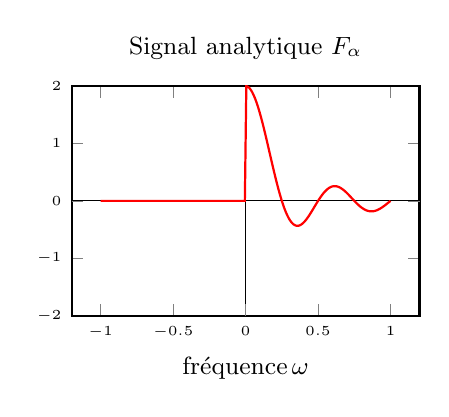
\begin{tikzpicture}
    \begin{axis}[
        title={Signal analytique $F_{\alpha}$},
        title style={font=\small},
        axis lines=box,
        style=thick,
        xlabel=\(\textnormal{fréquence}\, \omega\),
        xtick={-1, -0.5, 0.5, 1},
        ytick={-2, -1, 1, 2},
        extra x ticks=0,
        extra y ticks=0,
        extra x tick style={grid=major, grid style={black}},
        extra y tick style={grid=major, grid style={black}},
        tick label style={font=\tiny},
        label style={font=\small},
        ymin=-2, 
        ymax=2,
        ]
    \addplot[
        color=red,
        domain=-1:1,
        samples=200
        ]
    {(1+sign(x))*sin(360*x*2)/ (2*pi*x*2)};
    \end{axis}
    \end{tikzpicture}

    \caption[Signal analytique pour un signal simple]{Création du signal analytique dans le domaine fréquentiel (seule la partie réelle est montrée). Le signal original réel (gauche), qui présente une symétrie hermitienne, est ajouté à sa transformée de Hilbert (milieu), lui impair, pour former le signal analytique (droite), dépourvu de fréquence négative.}
    \label{fig:complex-analytic-representation}
\end{figure}

La suppression des composantes de fréquences peut être vue comme l'ajout d'un certain signal impair au signal de base.

\begin{equation} \label{eq:2.1}
    F_{\alpha}(\omega) = F(\omega) + F_h(\omega)
\end{equation}

La formation du signal analytique est montrée dans la figure~\ref{fig:complex-analytic-representation}. Dans l'équation~\ref{eq:2.1}, $F_h(\omega)$ est la « version impaire » du signal $F(\omega)$ :

\begin{equation}
    F_h(\omega) = \left\{
    \begin{array}{ll}
        F(\omega), & \omega > 0 \\
        -F(\omega), & \omega < 0 \\
        0, & \omega = 0,
    \end{array}
    \right.
\end{equation}

qui se reformule à l'aide de la fonction signe :

\begin{equation}
    F_h(\omega) = \sgn(\omega)\cdot F(\omega).
    \label{eq:2.5}
\end{equation}

L'expression de la fonction signe est la suivante :

\begin{equation}
    \sgn(x) = \left\{
    \begin{array}{ll}
        1, & x > 0 \\
        -1, & x < 0 \\
        0, & x = 0.
    \end{array}
    \right.
\end{equation}

L'équation~\ref{eq:2.1} est ainsi ré-écrite comme suit :

\begin{equation}
    F_{\alpha}(\omega) = (1+\sgn(\omega))F(\omega)
\end{equation}

\begin{figure}[h]
    %\noindent
    %\hspace{-10pt}
    \centering
    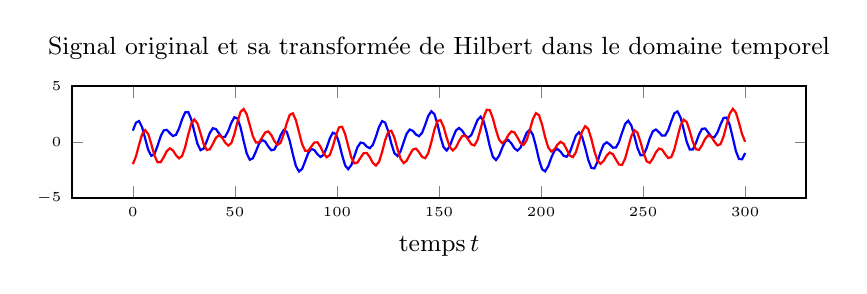
\begin{tikzpicture}
    \begin{axis}[
        title={Signal original et sa transformée de Hilbert dans le domaine temporel},
        title style={font=\small},
        axis lines=box,
        width=0.9\textwidth,
        height=3cm,
        style=thick,
        xlabel=\(\textnormal{temps}\, t\),
        xtick={0, 50, 100, 150, 200, 250, 300},
        ytick={-5, 0, 5},
        tick label style={font=\tiny},
        label style={font=\small},
        ymin=-5, 
        ymax=5,
        ]
    \addplot[
        color=blue,
        domain=0:300,
        samples=200
        ]
    {sin(3*x)+cos(15*x)+sin(30*x)};
    \addplot[
        color=red,
        domain=0:300,
        samples=200
        ]
    {-cos(3*x)+sin(15*x)-cos(30*x)};
    \end{axis}
    \end{tikzpicture}

    \caption[Signal analytique pour un signal complexe]{Exemple de représentation analytique. Le signal original réel (en bleu) et sa transformée de Hilbert imaginaire pure (en rouge).}
    \label{fig:analytic-representation}
\end{figure}

Le signal $F_{\alpha}$ créé est la somme dans le domaine fréquentiel de $F$, signal original pair, et de $F_h$, signal impair. Dans le domaine temporel, les représentations de $F$
et $F_h$ sont purement réelle et purement imaginaire respectivement. La représentation dans le domaine temporel de $F_h$ est nommée $f_h$. Dans le domaine temporel, $f_{\alpha}$ est donc un signal complexe sans composantes de fréquences négatives. $f_\alpha$ est un signal analytique et est appelé la représentation analytique de $f$ :

\begin{equation}
    f_{\alpha}(t) = \underbrace{f(t)}_\text{réel pur} + \underbrace{f_h(t)}_\text{imaginaire pur}.
\end{equation}

Le signal ajouté pour annuler les fréquences $F_h$ est par ailleurs un objet connu : c'est la transformée de Hilbert de $F$. Sa représentation, bien que très simple dans le domaine fréquentiel, est difficile à obtenir et manipuler dans le domaine temporel :

\begin{equation}
    f_h(t) = i \cdot \textnormal{p.v.} \int_{-\infty}^{\infty} \frac{f(t)}{\pi(t-\tau)} \,d\tau,
\end{equation}

où p.v. est la valeur principale de Cauchy. Cette intégrale représente la convolution avec la distribution $\frac 1{\pi t}$. L'intégrale est impropre à cause de la singularité en $t=\tau$. La valeur principale est nécessaire pour définir correctement cet objet. Dû à la complexité de l'intégrale, l'expression fréquentielle de la transformée de Hilbert est utilisée à la place :

\begin{align*}
    &\hil(F) = F_h = \sgn\cdot F \\
\end{align*}


\subsubsection{Amplitude et phase locales}

Pour comprendre l'intérêt du signal analytique, l'exemple d'une fonction sinusoïdale, d'amplitude $A$ et de fréquence $\omega_0$ fixées est présenté :

\begin{equation}
    f(t) = A\sin(\omega_0t).
\end{equation}

La transformée de Hilbert de $f$ est calculée en utilisant les relations présentées précédemment, ce qui donne la représentation analytique du signal :

\begin{align}
    f_h(t) &= iA\cos(\omega_0t) \\
    f_{\alpha}(t) &= f(t) + f_h(t) \\
    &= A\sin(\omega_0t)+iA\cos(\omega_0t) \\
    &= Ae^{i\omega_0t}.
\end{align}

Pour une sinusoïde, la transformée de Hilbert est un simple déphasage de $-\frac{\pi}2$ du signal original. Or la théorie de Fourier indique que n'importe quel signal générique peut être décomposé comme une somme de sinusoïdes. La transformée de Hilbert agit donc de la même manière sur tous les signaux : c'est un déphasage de $-\frac{\pi}2$ de chaque composante fréquentielle qui compose le signal. Le signal $f$ et sa transformée de Hilbert $f_h$ sont dits en quadrature de phase. Le signal analytique s'exprime comme une exponentielle complexe.

\bigskip

Puisque tout signal est représenté comme la somme d'un réel et d'un imaginaire pur, il est possible d'utiliser une représentation en coordonnées polaires pour exprimer l'exponentielle complexe. L'amplitude et la phase du signal sont alors variables au cours du temps :

\begin{equation}
    f_{\alpha} (t) = A(t)e^{i\phi(t)}.
\end{equation}

avec 

\begin{align}
    A(t) &= \sqrt{f(t)^2 + h_h(t)^2} \\
    \phi(t) &= \arctan\left(\frac{f_h(t)}{f(t)}\right).
\end{align}

Cette représentation introduit le concept d' amplitude locale et de phase locale (ici temporellement locales). L'amplitude et la phase locales sont deux outils d'analyse particulièrement intéressants pour l'étude approfondie du signal original. L'amplitude locale agit comme une mesure de l'enveloppe du signal. La phase locale agit comme une mesure de la forme du signal. Par exemple, une phase de $0$ indique un extremum, et une phase de $\pm\pi$ indique un passage par zéro. La figure~\ref{fig:local-pha-amp} montre un signal avec son amplitude locale et sa phase locale. À partir uniquement du signal initial, de l'information sur des caractéristiques et sur l'apparence du signal est obtenue.

\begin{figure}[h]

    \centering
    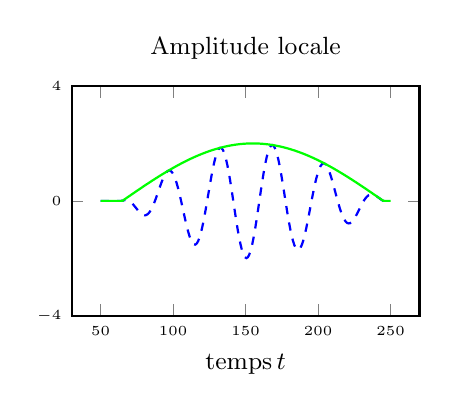
\begin{tikzpicture}
    \begin{axis}[
        title={Amplitude locale},
        title style={font=\small},
        axis lines=box,
        %width=0.9\textwidth,
        %height=3cm,
        style=thick,
        xlabel=\(\textnormal{temps}\, t\),
        xtick={50, 100, 150, 200, 250},
        ytick={-4, 0, 4},
        tick label style={font=\tiny},
        label style={font=\small},
        ymin=-4, 
        ymax=4,
        ]
    \addplot[
        color=blue,
        domain=50:250,
        samples=200,
        style=dashed,
        ]
    {(sign(x-65)-sign(x-245))*sin(10*x+25)*cos(x+25)};
    \addplot[
        color=green,
        domain=50:250,
        samples=200
        ]
    {(sign(x-65)-sign(x-245))*sqrt((0.5*(sin(11*x-40) + sin(9*x-90)))^2 + (sin(10*x+25)*cos(x+25))^2)};
    \end{axis}
    \end{tikzpicture}
    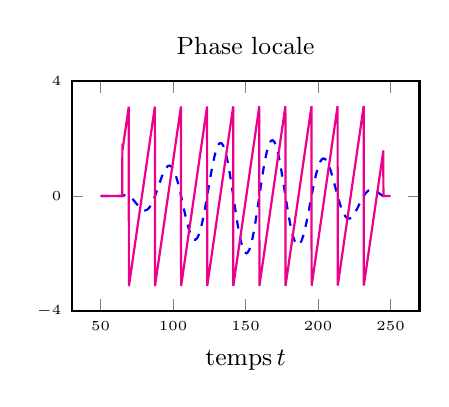
\begin{tikzpicture}
    \begin{axis}[
        title={Phase locale},
        title style={font=\small},
        axis lines=box,
        %width=0.9\textwidth,
        %height=3cm,
        style=thick,
        xlabel=\(\textnormal{temps}\, t\),
        xtick={50, 100, 150, 200, 250},
        ytick={-4, 0, 4},
        tick label style={font=\tiny},
        label style={font=\small},
        ymin=-4, 
        ymax=4,
        ]
    \addplot[
        color=blue,
        domain=50:250,
        samples=200,
        style=dashed,
        ]
    {(sign(x-65)-sign(x-245))*sin(10*x+25)*cos(x+25)};
    \addplot[
        color=magenta,
        domain=50:250,
        samples=2000
        ]
    {(sign(x-65)-sign(x-245))*rad(atan((0.5*(sin(11*x-40) + sin(9*x-90))) / (sin(10*x+25)*cos(x+25))))};
    \end{axis}
    \end{tikzpicture}

    \caption[Informations locales pour un signal simple]{Extraction d'informations locales pour un cosinus modulé par un sinus. L'amplitude locale (gauche) donne l'enveloppe de la sinusoïde, et la phase locale (droite) donne de l'information quant à la position dans le cycle d'oscillation.}
    \label{fig:local-pha-amp}

\end{figure}

\subsubsection{Notion d'échelle}
\label{subsubsec:echelle}

L'exemple donné avec la figure~\ref{fig:local-pha-amp} fonctionne bien car le signal est simple. L'interprétation de l'amplitude et la phase locale est claire et visuelle. Pour un signal plus complexe, plus représentatif des signaux étudiés, l'interprétation des informations locales est moins directe. La figure~\ref{fig:complex-local-pha-amp} affiche les informations locales du signal de la figure~\ref{fig:analytic-representation}, une somme de trois sinusoïdes de fréquences différentes. Les informations locales semblent décorrélées du signal complexe, ou le lien n'est pas directement apparent.

\bigskip

\begin{figure}[h]
    \centering
    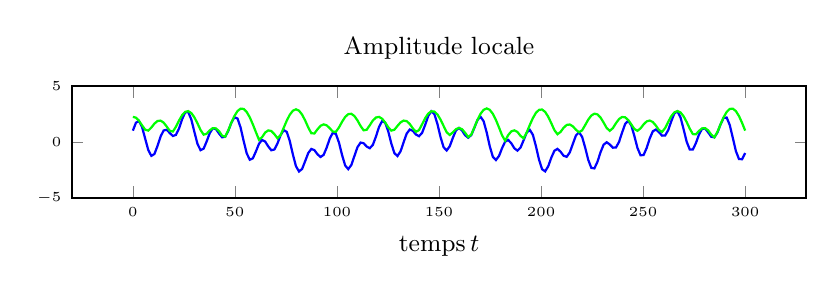
\begin{tikzpicture}
    \begin{axis}[
        title={Amplitude locale},
        title style={font=\small},
        axis lines=box,
        width=0.9\textwidth,
        height=3cm,
        style=thick,
        xlabel=\(\textnormal{temps}\, t\),
        xtick={0, 50, 100, 150, 200, 250, 300},
        ytick={-5, 0, 5},
        tick label style={font=\tiny},
        label style={font=\small},
        ymin=-5, 
        ymax=5,
        ]
    \addplot[
        color=blue,
        domain=0:300,
        samples=200
        ]
    {sin(3*x)+cos(15*x)+sin(30*x)};
    \addplot[
        color=green,
        domain=0:300,
        samples=200
        ]
    {sqrt((sin(3*x)+cos(15*x)+sin(30*x))^2 + (-cos(3*x)+sin(15*x)-cos(30*x))^2)};
    \end{axis}
    \end{tikzpicture}
    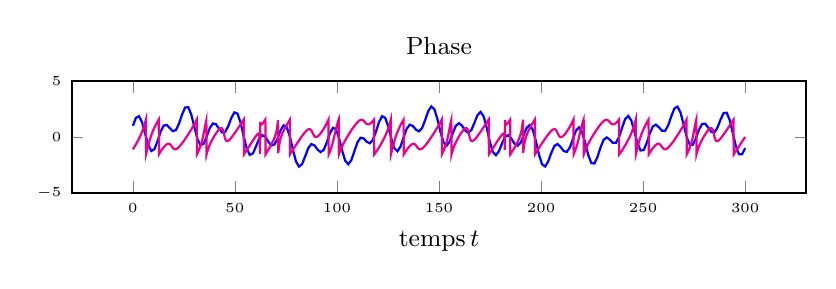
\begin{tikzpicture}
    \begin{axis}[
        title={Phase},
        title style={font=\small},
        axis lines=box,
        width=0.9\textwidth,
        height=3cm,
        style=thick,
        xlabel=\(\textnormal{temps}\, t\),
        xtick={0, 50, 100, 150, 200, 250, 300},
        ytick={-5, 0, 5},
        tick label style={font=\tiny},
        label style={font=\small},
        ymin=-5, 
        ymax=5,
        ]
    \addplot[
        color=blue,
        domain=0:300,
        samples=200
        ]
    {sin(3*x)+cos(15*x)+sin(30*x)};
    \addplot[
        color=magenta,
        domain=0:300,
        samples=3000
        ]
    {rad(atan((-cos(3*x)+sin(15*x)-cos(30*x)) / (sin(3*x)+cos(15*x)+sin(30*x))))};
    \end{axis}
    \end{tikzpicture}    

    \caption[Informations locales pour un signal complexe]{Informations locales pour un signal complexe, somme de plusieurs sinusoïdes. Pour un tel signal, l'interprétation des informations locales est moins directe.}
    \label{fig:complex-local-pha-amp}
\end{figure}

Le problème à l'analyse de ce signal est le fait qu'il existe plusieurs niveaux de structure, comme expliqué dans la section~\ref{subsec:structure}. Les différents niveaux de structure interfèrent et rendent l'interprétation des informations locales impossible à l'échelle macroscopique. Pour extraire de l'information interprétable, il faut sélectionner et faire l'analyse d'un seul niveau de structure, donc d'échelle. Un filtrage est fait pour sélectionner un niveau de structure en particulier et enlever les composantes des niveaux non désirés. Pour filtrer les niveaux de structure, il est possible d'utiliser des filtres passe-bande. Les filtres log-Gabor, utilisés par Bridge, sont un choix commun pour ce genre de pratique. Un filtre log-Gabor permet de sélectionner une bande de fréquence centrée autour d'une fréquence centrale $\omega_0$. Les filtres log-Gabor sont définis dans le domaine fréquentiel et ont une réponse en fréquence de forme gaussienne quand observés en échelle logarithmique :

\begin{equation}
    G(\omega) = \exp\left(-\frac{\log^2(\frac{|\omega|}{\omega_0})}{2\log(\sigma_0)^2}\right).
\end{equation}

Ces filtres sont caractérisés par deux paramètres : la fréquence centrale $\omega_0$ et et la largeur de bande $\sigma_0$. La fréquence centrale contrôle quelle échelle de structure est sélectionnée. La largeur de bande est un paramètre de forme qui contrôle la largeur de la bande de fréquence sélectionnée. Des exemples de filtre log-Gabor sont montrés à la figure~\ref{fig:log-gabor-filters}.

\bigskip

Le filtre log-Gabor est appliqué au signal avant de lui appliquer la transformée de Hilbert et de déterminer sa forme analytique. Le signal filtré offre une représentation locale en fréquence, centrée autour d'une fréquence $\omega_0$ et d'une échelle $\sigma_0$ variable arbitrairement.

\begin{equation}
    F_{\alpha}(\omega) = (1+\sgn(\omega))G(\omega)F(\omega)
\end{equation}

\begin{figure}
    \centering
    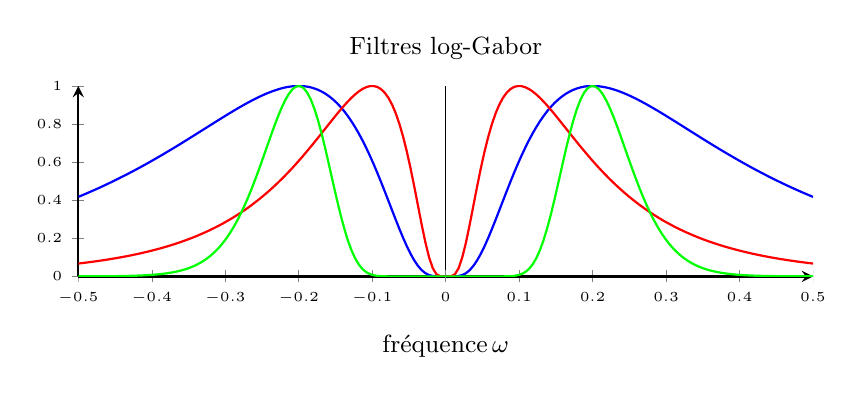
\begin{tikzpicture}
    \begin{axis}[
        title={Filtres log-Gabor},
        title style={font=\small},
        axis lines=left,
        width=0.9\textwidth,
        height=4cm,
        style=thick,
        xlabel=\(\textnormal{fréquence}\, \omega\),
        xtick={-0.5, -0.4, -0.3, -0.2, -0.1, 0.1, 0.2, 0.3, 0.4, 0.5},
        ytick={0, 0.2, 0.4, 0.6, 0.8, 1},
        tick label style={font=\tiny},
        label style={font=\small},
        extra x ticks=0,
        extra x tick style={grid=major, grid style={black}},
        ymin=0,
        ymax=1,
        ]
    \addplot[
        color=blue,
        domain=-0.5:0.5,
        samples=200
        ]
    {exp(-ln(abs(x)/.2)^2 / (2*ln(.5)^2))};
    \addplot[
        color=red,
        domain=-0.5:0.5,
        samples=200
        ]
    {exp(-ln(abs(x)/.1)^2 / (2*ln(.5)^2))};
    \addplot[
        color=green,
        domain=-0.5:0.5,
        samples=200
        ]
    {exp(-ln(abs(x)/.2)^2 / (2*ln(.8)^2))};
    \end{axis}
    \end{tikzpicture}

    \caption[Filtres log-Gabor]{Représentation dans le domaine fréquentiel de filtres log-Gabor de différents paramètres. En rouge, $\omega_0=0.1, \sigma_0 = 0.5$. En bleu, $\omega_0=0.2, \sigma_0 = 0.5$. En vert, $\omega_0=0.2, \sigma_0 = 0.8$.}
    \label{fig:log-gabor-filters}
\end{figure}

Étudier la réponse du signal sur une large gamme de fréquences et d'échelles offre une représentation locale du signal à différentes échelles. La représentation du signal à différentes échelles permet d'extraire de l'information sur les différentes structures du signal. Les informations locales sont présentées dans un graphique appelé scalogramme. Le scalogramme montre la réponse d'un signal en fonction du temps et de l'échelle, comme montré à la figure~\ref{fig:scalogram}. Les différents niveaux de structure du signal y sont visibles. Choisir le niveau d'échelle étudié donne un meilleur sens à l'interprétation des informations locales.

\bigskip

Les informations obtenues avec le signal analytique sont différentes de celles obtenues avec la transformée de Fourier. Les informations des deux modèles diffèrent et se complètent. La transformée de Fourier donne de l'information globale sur tout le signal, mais localisée en termes de fréquence. La représentation analytique, elle, donne une information spatialement locale sur le signal, mais sur une bande de fréquences sélectionnée par un filtre passe-bande. Le modèle d'information locale est donc un compromis entre la localisation spatiale et fréquentielle.


\begin{figure}
    \centering
    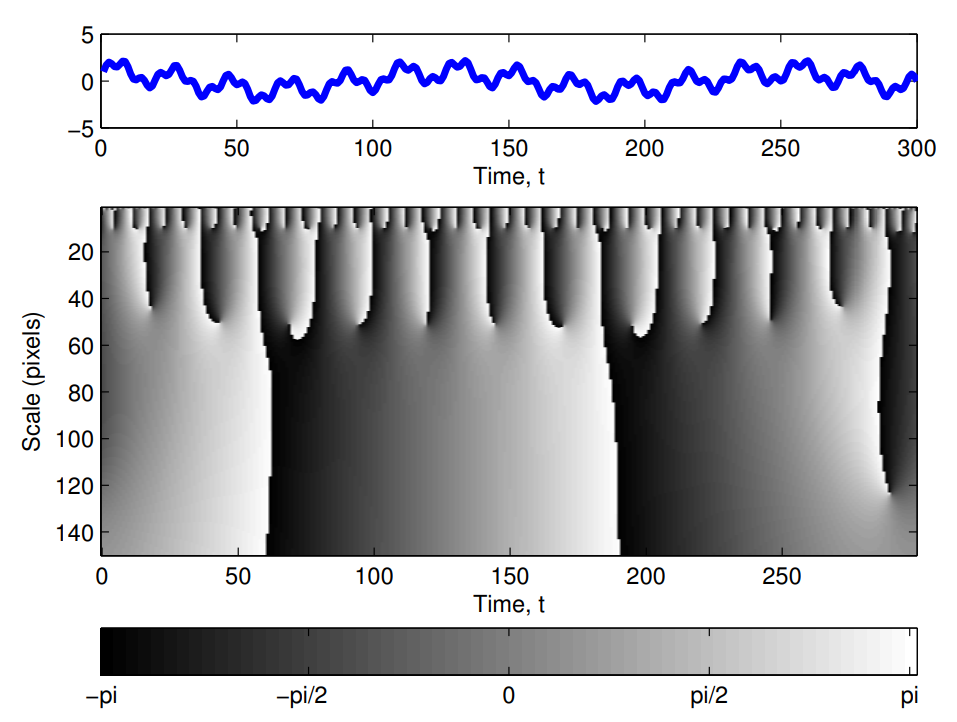
\includegraphics[width=\textwidth]{contenu/resources/images/scalogram}
    \caption[Scalogramme de la phase locale]{Scalogramme de la phase locale pour un signal complexe. La phase locale est représentée en échelle de gris et varie en fonction du temps (en abscisse) et de l'échelle en nombre de pixels (en ordonnée). Diagramme par Bridge~\cite{bridge_introduction_2018}.}
    \label{fig:scalogram}
\end{figure}


\subsection{Deux dimensions, signal monogène}

Le modèle du signal analytique permet l'extraction d'informations locales pour des signaux 1D. Il serait intéressant d'accéder à ces informations pour des images, des signaux 2D. En effet l'importance de la phase dans l'analyse d'image est connue depuis longtemps~\cite{oppenheim_importance_1981}. Cependant, l'application n'est pas directe dans le cas de deux (ou plus) dimensions, car il y a une notion de direction à considérer. Le modèle du signal monogène, proposé par Felsberg et Sommer~\cite{felsberg_monogenic_2001}, permet de prendre en compte la direction. La dérivation de ce modèle est expliquée dans cette partie.

\subsubsection{Construction du signal monogène}

Pour créer la représentation analytique d'un signal 1D, un imaginaire pur en quadrature de phase avec le signal original est ajouté au signal. La transformée de Hilbert est utilisée pour former le signal analytique. Pour un signal 2D, deux parties imaginaires sont nécessaires, une pour chaque direction. Il n'est donc pas possible de représenter le signal monogène comme un complexe. Pour un traitement exact, il faudrait utiliser les quaternions. Les quaternions peuvent être vus comme une extension des nombres complexes à une plus haute dimension. Pour simplifier la compréhension et manipulation, il est cependant possible se passer de la théorie des quaternions. Le signal monogène est traité comme s'il avait trois parties réelles distinctes dans un premier temps.

\bigskip

Pour générer les parties impaires du signal, une généralisation de la transformée de Hilbert est utilisée. La transformée de Riesz généralise la transformée de Hilbert à plusieurs dimensions et permet l'expression du signal analytique pour des signaux multi-dimensionnels. Soit $f$ un signal d'un espace 2D de la variable $\mathbf{x} = (x, y)^T$ et $F$ sa représentation dans le domaine fréquentiel obtenue par transformée de Fourier 2D, avec $\mathbf{\omega}=(\omega_x, \omega_y)^T$ une fréquence 2D. Alors les parties impaires de $f$, $F_{o1}$ et $F_{o2}$, sont données par :

\begin{align}
    F_{o1}(\mathbf{\omega}) &= \widehat{\mathcal{R}_1(f)}(\mathbf{\omega}) =
        \left\{
        \begin{array}{ll}
            -i\frac{\omega_x}{||\omega||}F(\omega), & \omega > 0 \\
            0, & \omega = 0,
        \end{array}
        \right. \\
    F_{o2}(\mathbf{\omega}) &= \widehat{\mathcal{R}_2(f)}(\mathbf{\omega}) =
        \left\{
        \begin{array}{ll}
            -i\frac{\omega_y}{||\omega||}F(\omega), & \omega > 0 \\
            0, & \omega = 0.
        \end{array}
        \right.
    \label{eq:2.20}
\end{align}

Avec cette définition de $F_{o1}$ et $F_{o2}$, les signaux correspondant dans le domaine spatial sont des signaux à valeurs réelles. En effet un signal 2D à valeurs réelles $f$ a un spectre dont la partie réelle est paire et la partie imaginaire impaire, soit :

\begin{equation}
    Re\{F(\omega)\} = Re\{F(-\omega)\}, \quad Im\{F(\omega)\} = -Im\{F(-\omega)\}.
\end{equation}

Dans la définition~\ref{eq:2.20}, comme $F$ est le spectre d'un signal réel. $F_{o1}$ et $F_{o2}$ vérifient donc ces propriétés de symétrie. Les signaux correspondants dans le domaine spatial sont bien réels.

\bigskip

Les parties impaires sont des versions généralisées de la transformée de Hilbert~\ref{eq:2.5}. Les parties impaires prennent en compte la direction de la fréquence. Chaque composante fréquentielle des parties impaires est déphasée de $-\pi/2$ et mise à l'échelle de telle sorte que l'amplitude est partagée entre les deux parties.

\bigskip

\begin{figure}
    \centering
    \begin{subfigure}[b]{.3\textwidth}
        
\includegraphics[width=\textwidth]{contenu/resources/images/disk}
        \caption{Signal original}
    \end{subfigure}
    \hfill
    \begin{subfigure}[b]{.3\textwidth}
        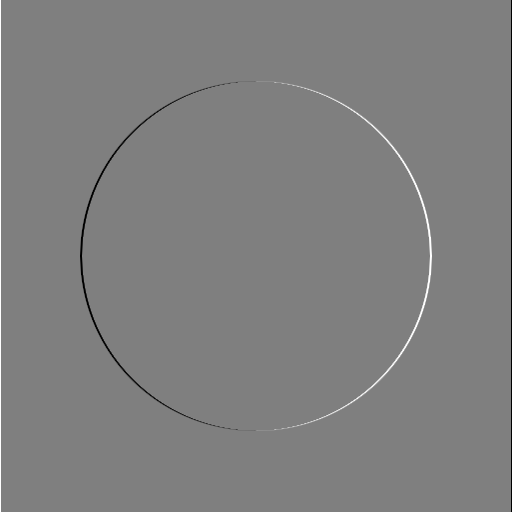
\includegraphics[width=\textwidth]{contenu/resources/images/r2_disk}
        \caption{Première partie impaire}
    \end{subfigure}
    \hfill
    \begin{subfigure}[b]{.3\textwidth}
        
\includegraphics[width=\textwidth]{contenu/resources/images/r1_disk}
        \caption{Seconde partie impaire}
    \end{subfigure}
    \caption[Visualisation du signal monogène pour un disque]{Visualisation du signal monogène pour un disque : le signal original $f$ (gauche) et ses parties impaires $f_{o1}$ (milieu) et  $f_{o2}$ (droite), affichées avec une échelle de couleurs encodant la valeur, de -1 (noir) à +1 (blanc).}
    \label{fig:monogenic-signal-disk}
\end{figure}

Le signal monogène est alors exprimé comme un vecteur à trois composantes, une paire et deux impaires :

\begin{equation}
    f_m(\mathbf{x}) =
    \left[
        \begin{array}{c}
        f_e(\mathbf{x}) \\
        f_{o1}(\mathbf{x}) \\
        f_{o2}(\mathbf{x})
        \end{array}
    \right],
\end{equation}

où $f_e$ est le signal original, indexé par un $e$ pour souligner qu'il représente la partie paire du signal monogène. Une représentation d'un signal et de ses parties impaires est montrée à la figure~\ref{fig:monogenic-signal-disk}. Dans la figure, les parties impaires détectent des changements verticaux et horizontaux dans le signal. La détection des changements est due au fait que la transformée de Riesz présente une ressemblance et une connexion au gradient (l'équation~\ref{eq:2.20} rappelle fortement la définition du gradient, à un facteur près). La transformée de Hilbert présente d'ailleurs aussi une connexion au gradient en 1D. La relation entre les transformées étudiées et le gradient n'est pas le sujet de cette étude et n'est pas explorée plus en profondeur. La personne intéressée se référera à Unser \textit{et al.}\cite{unser_multiresolution_2009} pour plus de détails.

\bigskip

Il est aussi commun de se représenter le signal monogène comme un vecteur de deux composantes seulement, une paire et une impaire. La composante impaire est alors une combinaison des deux parties impaires présentées ici. Cette représentation est plus compacte, au détriment de la perte d'information sur l'orientation. Elle sera parfois utilisée dans la suite de ce travail :

\begin{equation}
    f_o(\mathbf{x}) = \sqrt{f_{o1}(\mathbf{x})^2 + f_{o2}(\mathbf{x})^2}.
\end{equation}

La transformée de Riesz peut s'exprimer directement dans le domaine spatial. Comme la transformée de Hilbert, la représentation spatiale de la transformée de Riesz est un objet mathématique compliqué, une intégrale singulière :

\begin{equation}
    R_if(x) = c_d \lim_{\epsilon \to 0}\int_{\mathbb{R}^d\setminus B_\epsilon(x)}\frac{(x_i-t_i)f(t)}{|x-t|^{d+1}}\,dt,
    \label{eq:riesz-transform-spatial}
\end{equation}

pour $i\in\llbracket 0, d\rrbracket$ avec $d$ la dimension. $c_d$ est une constante de normalisation dimensionnelle :

\begin{equation}
    c_d = \frac1{\pi\omega_{d-1}} = \frac{\Gamma((d+1)/2)}{\pi^{(d+1)/2}},
\end{equation}

avec $\omega_{d-1}$ le volume de la $(d-1)$-sphère unité. Au vue de la complexité de calcul et de manipulation de cette expression, la formulation fréquentielle est utilisée dans la suite du travail.

\subsubsection{Amplitude, phase et orientation locales}

Avec le signal monogène, le concept d'informations locales est maintenant dérivable pour des images. En 1D, les deux parties du signal analytiques sont représentées en coordonnées polaires avec l'amplitude et la phase. En 2D il y a trois parties à représenter. Les coordonnées sphériques sont donc utilisées. En coordonnées sphériques trois composantes sont définies : le rayon, l'angle d'élévation et l'azimut, comme montré en figure~\ref{fig:spherical-representation}.

\bigskip

\begin{figure}
    \centering
    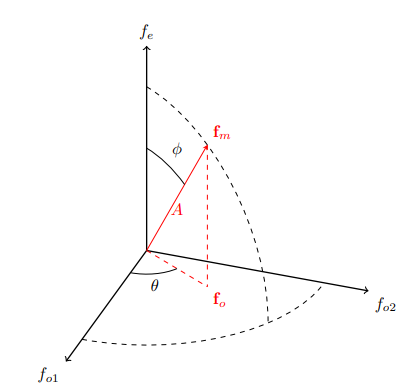
\includegraphics[width=.45\textwidth]{contenu/resources/images/spherical_representation}
    \caption[Représentation du signal monogène en coordonnées sphériques]{Représentation du signal monogène $f_m$ (rouge) en coordonnées sphériques, où les axes sont les différentes parties du signal. Le rayon représente l'amplitude locale, l'angle d'élévation $\phi$ la phase locale et l'azimut $\theta$ l'orientation locale.}
    \label{fig:spherical-representation}
\end{figure}

L'amplitude locale $A$ représente, comme en 1D, le rayon de la représentation :

\begin{align}
    A(\mathbf{x}) &= \sqrt{f_e(\mathbf{x})^2 + f_{o1}(\mathbf{x})^2 + f_{o2}(\mathbf{x})^2} \\
    &= \sqrt{f_e(\mathbf{x})^2 + f_o(\mathbf{x})^2}.
\end{align}

La phase locale $\phi$ mesure l'angle entre la partie paire $f_e$ et la partie impaire combinée $f_o$. La phase représente ainsi l'angle d'élévation de la représentation :

\begin{equation}
    \phi(\mathbf{x}) = \arctan\left(\frac{f_o(\mathbf{x})}{f_e(\mathbf{x})}\right).
\end{equation}

Enfin l'orientation locale $\theta$ complète la représentation en donnant l'angle d'azimut. L'orientation locale indique la direction dominante dans l'image à cet endroit, exprimée comme l'orientation de la partie impaire $f_o$ :

\begin{equation}
    \theta(\mathbf{x}) = \arctan\left(\frac{f_{o2}(\mathbf{x})}{f_{o1}(\mathbf{x})}\right).
\end{equation}

La figure~\ref{fig:monogenic-local-representation} montre un exemple de représentation locale pour une image, avec l'amplitude, la phase et l'orientation locales.

\bigskip

\begin{figure}
    \centering
    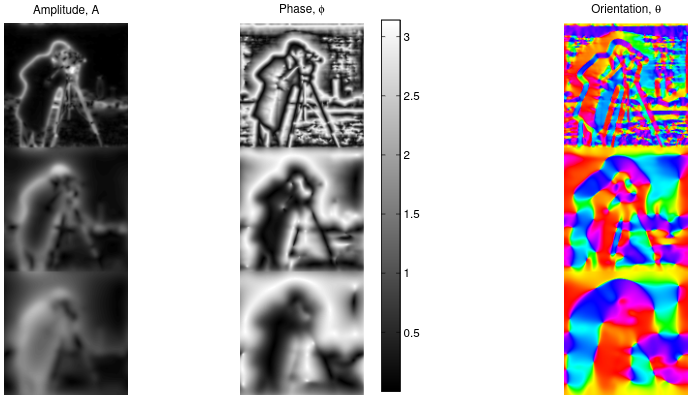
\includegraphics[width=\textwidth]{contenu/resources/images/local_information_monogenic}
    \caption[Représentation locale du signal monogène]{Représentation locale du signal monogène pour une image, avec l'amplitude (gauche), la phase (milieu) et l'orientation (droite) locales. Image par Bridge~\cite{bridge_introduction_2018}.}
    \label{fig:monogenic-local-representation}
\end{figure}

Le changement de représentation est réversible. Le signal monogène peut être reconstruit à partir de ses informations locales :

\begin{equation}
    f_m(\mathbf{x}) = A(\mathbf{x})\left[
        \begin{array}{c}
        \cos(\phi(\mathbf{x})) \\
        \sin(\phi(\mathbf{x}))\cos(\theta(\mathbf{x})) \\
        \sin(\phi(\mathbf{x}))\sin(\theta(\mathbf{x}))
        \end{array}
    \right].
\end{equation}

Notamment, l'image originale s'exprime simplement par $f(\mathbf{x}) = A(\mathbf{x})\cos(\phi(\mathbf{x}))$. Cette formule est utilisée plus tard dans ce travail pour reconstruire les images après modification de leurs informations locales.

\bigskip

Comme pour le signal analytique en 1D, des filtres peuvent être utilisés pour sélectionner un niveau d'échelle à analyser. Sélectionner un niveau d'échelle permet ici encore d'extraire de l'information sur certains niveaux de structure en particulier. Les filtres log-Gabor peuvent être étendus en 2D et utilisés pour sélectionner certaines parties du signal~\ref{fig:2D-log-gabor}.

\bigskip

\begin{figure}
    \centering
    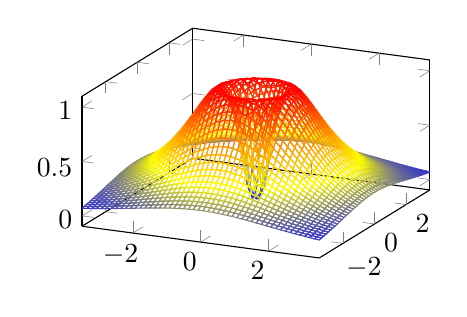
\begin{tikzpicture}
    \begin{axis}[
        colormap/hot,
%        xtick={-.5, 0, .5},
%        ytick={-.5, 0, .5},
%        ztick={-1, 0, 1}
    ]
        \addplot3[
        mesh,
        samples=50,
        domain=-3.5:3.5,
        ]
        {exp(-(ln(sqrt(x^2+y^2))^2)/(2*ln(.5)^2))};
    \end{axis}
    \end{tikzpicture}

    \caption[Filtre log-Gabor en 2D]{Représentation en domaine fréquentiel d'un filtre log-Gabor. Comme en 1D, le filtre sélectionne une bande de fréquence centrée autour d'une fréquence centrale $\omega_0$ et de largeur de bande $\sigma_0$.}
    \label{fig:2D-log-gabor}
\end{figure}

Les parties paires et impaires du signal sont calculées en sélectionnant plusieurs échelles différentes. Les représentations locales créées à chaque niveau d'échelle mettent en valeur les différents niveaux de structure présents dans l'image. La figure~\ref{fig:cameraman-monogenic} montre une image et son signal monogène, calculé sur plusieurs niveaux d'échelle.

\begin{figure}
    \centering
    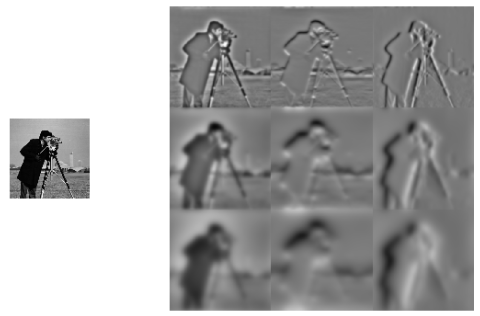
\includegraphics[width=.75\textwidth]{resources/images/cameraman_monogenic}
    \caption[Signal monogène calculé pour plusieurs niveaux d'échelle]{Image originale (gauche) et son signal monogène (droite), calculé sur plusieurs niveaux d'échelle. Dans l'image de droite : en colonne les différentes parties, paire $f_e$ (gauche), impaire 1 $f_{o1}$ (milieu) et impaire 2 $f_{o2}$ (droite). En ligne les longueurs d'onde centrale $\lambda_0 = 2\pi/\omega_0$, caractéristiques de l'échelle de structure détectée : $\lambda_0 = 20$~pixels (haut), $\lambda_0 = 60$~pixels (milieu), $\lambda_0 = 100$~pixels (bas). Pour référence, la taille de l'image originale est 256 $\times$ 256 pixels. Image par Bridge~\cite{bridge_introduction_2018}.}
    \label{fig:cameraman-monogenic}
\end{figure}

\bigskip

Le cadre de travail pour le restant du manuscript, le signal monogène, a été introduit. Le cadre choisi pour travailler à différents niveaux de structure va maintenant être discuté. Bridge présente dans son article~\cite{bridge_introduction_2018} un cadre de travail utilisant les filtres log-Gabor. Les filtres log-Gabor 2D possèdent une expression complexe dans le domaine spatial. Pour les travaux présentés, une autre méthode de représentation est utilisée : la pyramide de Riesz. Les calculs nécessaires à la création et manipulation de la pyramide de Riesz sont plus élémentaires que ceux des filtres log-Gabor. Le choix de la simplicité pour les calculs permet de concentrer les efforts de recherche sur l'analyse de textures. La section qui suit introduit la pyramide de Riesz et montre comment elle peut être utilisée pour l'analyse de textures.

\section{Pyramide de Riesz}

L'idée de travailler en considérant plusieurs niveaux d'échelle est introduite par Burt et Adelson~\cite{burt_laplacian_1983} pour la compression d'images. La méthode de la pyramide d'image mise au point par Burt et Adelson est une méthode de représentation multi-échelle utilisée dans les domaines de la vision par ordinateur et du traitement d'image pour la résolution de nombreux problèmes comme la détection de motifs. Une pyramide d'images remplit la même fonction qu'une banque de filtres, comme les filtres log-Gabor utilisés par Bridge. Une image est décomposée en sélectionnant successivement différentes bandes de fréquences. De l'information localisée en fréquence est ainsi extraite.

\bigskip

La pyramide d'image est ensuite étendue par Simoncelli \textit{et al.}~\cite{simoncelli_shiftable_1992}. La pyramide de Simoncelli \textit{et al.}, dite orientable, a des propriétés d'invariance par rotation, translation et mise à l'échelle. Les propriétés d'invariance de la pyramide orientable sont une amélioration par rapport aux modèles précédent. La pyramide orientable sert de base à la pyramide de Riesz utilisée dans ces travaux. Wadhwa \textit{et al.}~\cite{wadhwa_phase_based_2013} mettent au point la pyramide de Riesz pour étudier les micro-mouvements dans des vidéos. La pyramide utilisée dans les travaux présentés est fortement inspirée de Wadhwa \textit{et al.} La construction de la pyramide, plus détaillée dans les paragraphes qui suivent, s'organise comme suit. Dans un premier temps les pyramides gaussienne puis laplacienne sont formées. La pyramide laplacienne offre une méthode de reconstruction de l'image. La transformée de Riesz est ensuite appliquée à tous les étages de la pyramide pour obtenir le signal monogène de chaque niveau. Les informations locales des différents niveaux sont enfin extraites pour analyser les différents niveaux de structure. La pyramide de Riesz est un outil d'analyse qui sera par la suite utilisée pour l'analyse et la synthèse de textures.

\subsection{Pyramide gaussienne}

Il existe deux types principaux de pyramide, passe-bas et passe-bande. Pour créer une pyramide passe-bas, aussi dite gaussienne, deux étapes sont répétées itérativement :

\bigskip

\begin{itemize}
    \item une étape de lissage (ou filtrage) de l'image, qui consiste à appliquer un filtre passe-bas à l'image, afin de supprimer les hautes fréquences. Une image lissée est formée, où les détails fins ont été supprimés ;
    \item une étape de sous-échantillonnage, qui consiste à réduire la taille de l'image en gardant un pixel sur deux dans chaque direction. L'image obtenue a la moitié de la taille de l'image originale.
\end{itemize}

\bigskip

Les deux étapes sont répétées sur l'étage nouvellement créé, et ce jusqu'à atteindre la profondeur désirée. Le résultat est une collection d'images de plus en plus petites et de moins en moins raffinées (en termes de résolution). Un exemple est donné en figure~\ref{fig:gaussian-pyramid}. La collection d'images peut être représentée graphiquement comme une pyramide en superposant les étages du plus grand au plus petit, comme montré à la figure~\ref{fig:pyramid-gauss}.

\begin{figure}[h]
    \centering

    \begin{subfigure}{.3\textwidth}
        \centering
        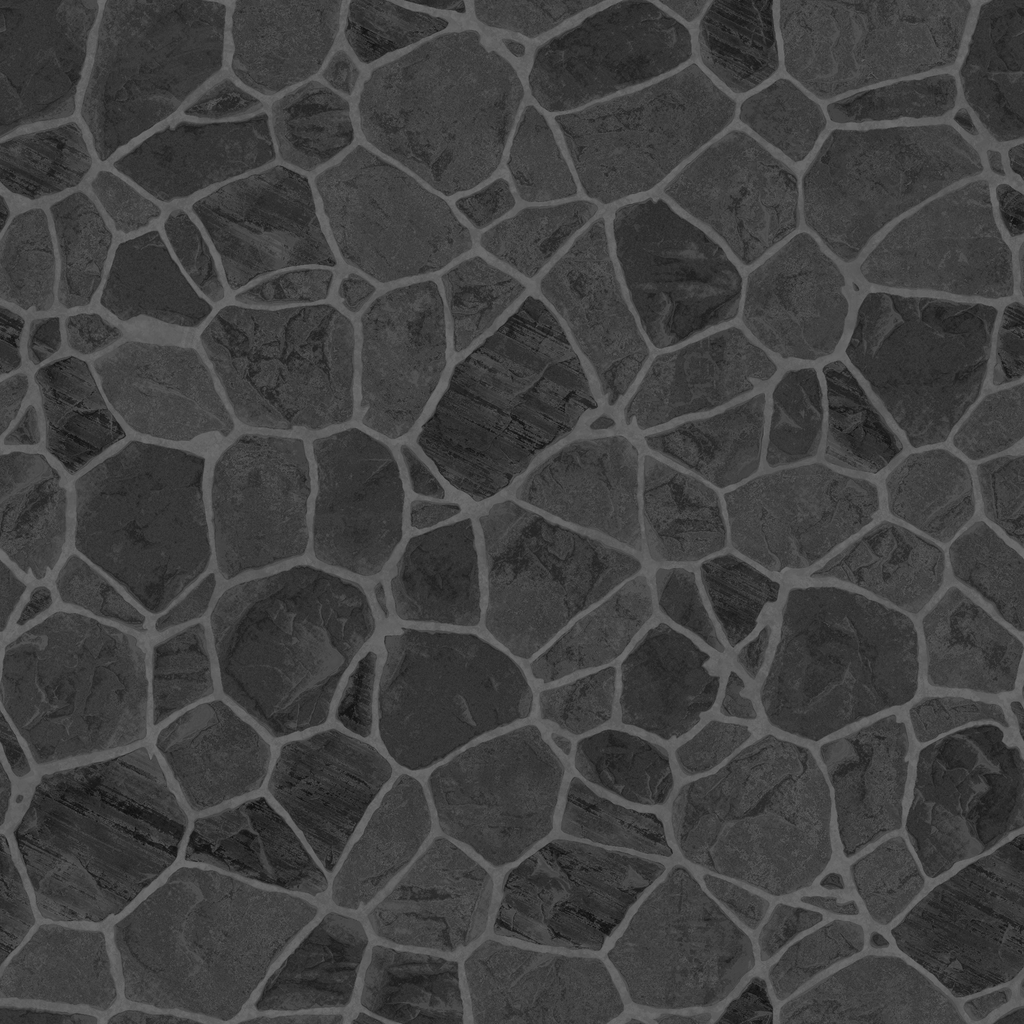
\includegraphics[width=\textwidth]{contenu/resources/images/gauss_0}
        \caption{Image originale}
    \end{subfigure}
    \hfill
    \begin{subfigure}{.3\textwidth}
        \centering
        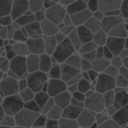
\includegraphics[width=\textwidth]{contenu/resources/images/gauss_3}
        \caption{Étage 3}
    \end{subfigure}
    \hfill
    \begin{subfigure}{.3\textwidth}
        \centering
        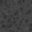
\includegraphics[width=\textwidth]{contenu/resources/images/gauss_5}
        \caption{Étage 5}
    \end{subfigure}
%    \hfill
%    \begin{subfigure}{.22\textwidth}
%        \centering
%        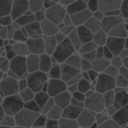
\includegraphics[width=\textwidth]{contenu/resources/images/gauss_3}
%        \caption{Étage 3}
%    \end{subfigure}

    \caption[Étages de la pyramide de Gauss]{Étages de la pyramide de Gauss. De gauche à droite, les étages sont de plus en plus petits.}
    \label{fig:gaussian-pyramid}
\end{figure}

Différents noyaux de lissage ont été proposés dans la littérature. La famille des noyaux binomiaux par exemple est fréquemment utilisée. L'implémentation proposée dans ce travail utilise les noyaux binomiaux, qui s'expriment à l'aide des coefficients binomiaux :

\begin{equation}
    k = \frac{1}{256}\left[
        \begin{array}{ccccccc}
            1 & 4 & 6 & 4 & 1 \\
            4 & 16 & 24 & 16 & 4 \\
            6 & 24 & 36 & 24 & 6 \\
            4 & 16 & 24 & 16 & 4 \\
            1 & 4 & 6 & 4 & 1
        \end{array}
    \right],
\end{equation}

Il est intéressant de constater que les pyramides gaussiennes sont notamment utilisées dans la synthèse de texture. En effet les MIP maps employées pour remédier au sous-échantillonnage sont un pré-calcul des textures à différents niveaux de résolution ; ce sont des pyramides gaussiennes.

\begin{figure}
    \centering
    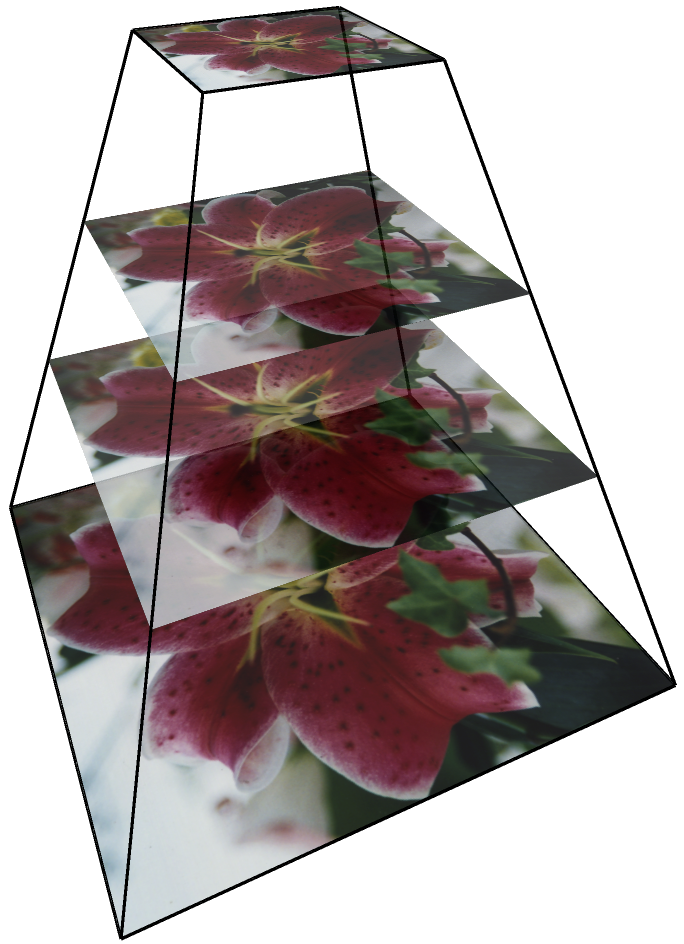
\includegraphics[width=.25\textwidth]{contenu/resources/images/image_pyramid_placeholder}
    \caption[Représentation pyramidale des étages de la pyramide de Gauss]{Représentation en pyramide des étages de la pyramide de Gauss. Crédit à \textit{Isnomore} pour l'image}
    \label{fig:pyramid-gauss}
\end{figure}

\subsection{Pyramide laplacienne}

La pyramide laplacienne est une autre forme de pyramide qui correspond à un type passe-bande. Comme l'expliquent Burt et Adelson~\cite{burt_laplacian_1983}, les texels voisins dans une image sont souvent hautement corrélés. Encoder une image en termes de valeur de pixels cause une perte d'efficacité à cause de la redondance d'information. Il est possible d'encoder une image plus efficacement, c'est-à-dire avec moins de bits. La pyramide laplacienne est une représentation qui décorelle les texels voisins et qui répond donc à cette problématique.

\subsubsection{Construction de la pyramide}

Plutôt que d'encoder la valeur même de chaque pixel, une prédiction est faite sur la valeur que chaque pixel devrait avoir. C'est l'erreur de prédiction qui est alors encodée. La valeur prédite de chaque pixel est obtenue en calculant une moyenne pondérée locale centrée autour du pixel. Dans un premier temps, une image lissée est créée par convolution. La convolution par filtre correspond au calcul de la moyenne pondérée. L'image lissée représente les corrélations locales entre les texels au niveau d'échelle correspondant au filtre choisi. L'image lissée comporte les éléments redondants à encoder plus efficacement. Pour améliorer l'encodage, l'image lissée est soustraire à l'image originale. L'image obtenue exprime l'erreur de prédiction pour chaque texel. La relation suivante illustre le procédé :

\begin{equation}
    L = I - k * I,
\end{equation}

avec $I$ l'image originale, $L$ l'image d'erreur de prédiction et $k$ le filtre de moyenne pondérée. Pour la compression d'images, l'intérêt se trouve dans cette ré-écriture. Les pixels de $L$ sont décorrélés et de faible valeur, donc encodables avec peu de bits. $k*I$ est une image lissée, qui peut être sous-échantillonnée pour obtenir une image de moitié de taille. L'image est représentée par $L$ et $k*I$ uniquement et cette représentation est plus compacte que l'image originale.

\bigskip

Le processus est répétable itérativement, en appliquant à chaque fois le même filtre à l'image lissée de résolution inférieure. La figure~\ref{fig:gauss-laplace-pyramid} illustre le processus itératif de construction de la pyramide laplacienne. Seules les images d'erreur, dont la taille est divisée par 4 à chaque fois, sont enregistrées. La dernière image lissée, est de taille $N/2^{2d}$, avec $N$ la taille de l'image initiale et $d$ la profondeur désirée. Encore une fois, la collection d'images est représentable comme une pyramide, en superposant les images de la plus grande à la plus petite.

\bigskip

Le filtre de lissage utilisé est un filtre passe-bas, qui moyenne localement l'image. Le même genre de filtre passe-bas est utilisé pour créer une pyramide gaussienne. En fait, une pyramide gaussienne est souvent utilisée pour construire une pyramide laplacienne. La pyramide gaussienne représente toutes les images lissées nécessaires à la construction de la pyramide laplacienne. La pyramide gaussienne est calculée, puis à chaque étage est soustrait l'étage de résolution inférieure. Les images d'erreur de prédiction sont obtenus à partir de la pyramide gaussienne.

\bigskip

Pour soustraire une image lissée à son image de taille originale, une étape d'expansion est nécessaire. Une méthode communément utilisée pour l'expansion consiste à doubler la taille de l'image, en insérant des zéros entre chaque pixel, puis à appliquer un filtre passe-bas à l'image résultante. L'image résultante est une image de taille double qui est une approximation de l'image lissée. Cette image est alors soustraite à l'image originale pour obtenir l'image d'erreur de prédiction.

\begin{figure}
    \centering
    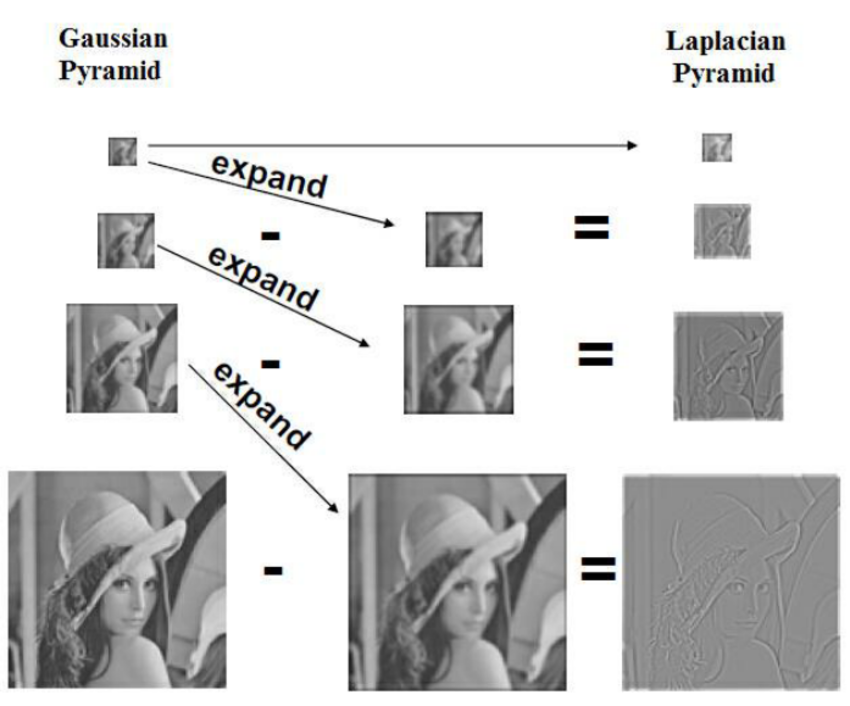
\includegraphics[width=.75\textwidth]{contenu/resources/images/gauss_laplace_pyramid}
    \caption[Relation entre pyramide gaussienne et laplacienne]{Processus de création de la pyramide laplacienne à partir de ma pyramide gaussienne. Crédit à \textit{Jebamalar et Sutha}~\cite{jebamalar_design_2014} pour l'image.}
    \label{fig:gauss-laplace-pyramid}
\end{figure}

\subsubsection{Reconstruction de l'image}

L'image décomposée en pyramide laplacienne est stockée en enregistrant les images d'erreur de prédiction et l'image lissée de plus basse résolution. Pour reconstruire l'image originale, un processus itératif est utilisé. Le résidu basse fréquences est additionné à la dernière image d'erreur pour former une image lissée de résolution supérieure. Le processus est répété en additionnant à chaque fois l'image lissée obtenue à l'image d'erreur suivante, jusqu'à obtenir l'image originale.

\bigskip

Avec une pyramide gaussienne, les images lissées sont de taille différente (divisée par 4 à chaque fois). Deux images doivent avoir la même taille pour pouvoir être soustraites l'une à l'autre. Pour s'assurer que les images ont la même taille, les images lissées sont étendues à chaque étape. La même opération d'expansion que celle de la création de la pyramide est utilisée pour étendre les images. Le processus de reconstruction est montré à l'image~\ref{fig:laplace-reconstruction}.

\begin{figure}
    \centering
    \includegraphics[width=.85\textwidth]{contenu/resources/images/laplacian_pyramid_reconstruction}
    \caption[Reconstruction d'une image à partir de sa pyramide laplacienne]{Reconstruction d'une image à partir de sa pyramide laplacienne. $f_i$ les images de la pyramide gaussienne, $h_i$ celles de la pyramide laplacienne, et $l_i$ les images lissées étendues. Image de \href{https://web.archive.org/web/20230203082428/http://sepwww.stanford.edu/data/media/public/sep/morgan/texturematch/paper_html/node3.html}{Stanford Exploration Project}.}
    \label{fig:laplace-reconstruction}
\end{figure}

\subsection{Pyramide de Riesz}

La pyramide de Riesz est une extension de la pyramide laplacienne. C'est le cadre permet l'étude du signal monogène d'une image à différents niveaux d'échelle. La pyramide de Riesz est construite en appliquant la transformée de Riesz à chaque étage de la pyramide laplacienne. La pyramide de Riesz est illustrée à la figure~\ref{fig:riesz-pyramid-cameraman}. Les informations locales sont ensuite calculées pour chaque étage de la pyramide. Les informations locales des différents niveaux sont mis en relation dans la suite des travaux afin plus d'information sur l'image, comme expliqué dans le chapitre implémentations~\ref{chap:chapitre2}.

\bigskip

\begin{figure}
    \centering
    \includegraphics[width=.65\textwidth]{contenu/resources/images/riesz_pyramid_cameraman}
    \caption[Pyramide de Riesz]{Différents étages de la pyramide de Riesz, calculée avec la transformée de Riesz approximée. En colonne, les différentes composantes : l'image originale de la pyramide laplacienne (gauche), puis les deux composantes de Riesz (milieu et droite). En ligne, les différents étages de la pyramide : étage 0 (haut), étage 2 (milieu) et étage 3, le dernier (bas).}
    \label{fig:riesz-pyramid-cameraman}
\end{figure}

Pour des raisons de vitesse de calcul et de simplicité d'implémentation, la vraie transformée de Riesz n'est pas utilisée dans ce travail. La transformée de Riesz nécessite une transformation de l'image dans le domaine de Fourier ou le calcul d'une intégrale singulière (voir l'équation~\ref{eq:riesz-transform-spatial}), deux méthodes qui sont complexes à opérationnaliser. À la place, l'approximation proposée par Wadhwa \textit{et al.}~\cite{wadhwa_riesz_2014} est utilisée. L'approximation de Wadhwa \textit{et al.} se calcule directement dans le domaine spatial en utilisant les filtres à réponse impulsionnelle finie $[-0.5, 0, 0.5]$ et $[-0.5, 0, 0.5]^T$, dont les réponses en fréquence sont :

\begin{equation}
    -i\sin(\omega_x) \quad \text{et} \quad -i\sin(\omega_y).
\end{equation}

Cette approximation donne de bons résultats ici, car les filtres ont une réponse équivalente à celle de la transformée de Riesz aux alentours de $\frac\pi2$, où se concentre la majorité de l'énergie des images dans la pyramide laplacienne~\cite{wadhwa_riesz_2014}. En $0$, il y a une différence notable entre la réponse des filtres et la réponse de la transformée de Riesz. Cependant, le contenu fréquentiel est faible en $0$ puisque, par construction, le contenu basse fréquences est supprimé dans la pyramide laplacienne. L'erreur due à la différence en $0$ est donc faible aussi. La figure~\ref{fig:riesz-approximation} montre une comparaison entre l'application de la transformée de Riesz et de son approximation. Les informations locales pour chaque étage, amplitude, phase et orientation, sont ensuite calculées comme expliqué dans la section précédente. La figure~\ref{fig:riesz-pyramid-local} présente les informations locales obtenues avec la pyramide de Riesz.

\bigskip

\begin{figure}[h]
    \centering
    \includegraphics[width=.65\textwidth]{contenu/resources/images/riesz_approximation}
    \caption[Approximation de la transformée de Riesz]{Comparaison de l'application de la transformée de Riesz (gauche) et de son approximation (droite) pour un niveau de pyramide. Les tranches horizontales en jaune sur les images (a) et (b) sont représentées dans le diagramme en (c). Image par Wadhwa \textit{et al.}~\cite{wadhwa_riesz_2014}.}
    \label{fig:riesz-approximation}
\end{figure}

\begin{figure}[hp]
    \centering
    \includegraphics[width=.90\textwidth]{contenu/resources/images/riesz_pyramid_pasta}
    \caption[Informations locales de la pyramide de Riesz]{Informations locales de la pyramide de Riesz. En colonne, les différentes composantes : en colonne, les différentes informations locales : amplitude (gauche), phase (milieu) et orientation (droite). En ligne les différentes étages de la pyramide, du premier (haut) au dernier (bas).}
    \label{fig:riesz-pyramid-local}
\end{figure}

Avec cette implémentation de la pyramide de Riesz, le cadre d'étude multirésolution local a été défini. La prochaine partie décrit comment le cadre multirésolution local est utilisé afin d'extraire de l'information d'une texture.

\section{Congruence de phases}

Le modèle de l'énergie locale est un modèle de détection de caractéristiques saillantes dans une image. Introduit par Morrone et al~\cite{morrone_mach_1986, morrone_feature_1987},il explique la présence de points saillants, tels que des bords et des coins, par l'alignement des phases locales de l'image. Le modèle d'énergie locale est basé sur l'observation que les bords et les coins sont des structures résultant de la superposition de sinusoïdes en phase les unes avec les autres. Contrairement aux autres méthodes de détection de caractéristiques, comme celles de Sobel ou Canny, le modèle de Morrone \textit{et al.} est insensible aux variations de luminosité et de grossissement. Les méthodes par gradient utilisent en effet un seuillage pour déterminer les bords, qui dépend de la luminosité et du niveau de zoom de l'image. À l'inverse, le modèle de l'énergie locale permet le calcul de la congruence de phases (PC), une grandeur à valeurs dans $[0, 1]$ mesurant uniformément la présence d'éléments caractéristiques dans une image et la proximité d'un texel à un élément caractéristique. La congruence de phases est le sujet de la partie qui suit.

\bigskip

La formulation initiale de la PC utilise les coefficients de la série de Fourier du signal. Cependant, cette formulation comporte trois problèmes : elle est difficile à calculer et manipuler, elle ne permet pas une bonne localisation de l'information (le même problème qui pousse à utiliser un cadre de travail multirésolution pour l'étude du signal monogène), et elle ne prend pas en compte la répartition des fréquences. Ces problèmes et leur solution sont expliqués dans un premier temps en 1D, puis en 2D.

\subsubsection{Énergie locale}

Venkatesh et Owens~\cite{venkatesh_energy_1989} montrent qu'il existe une relation directe entre la PC et l'énergie locale. Ils mettent ainsi en lumière une expression simplifiée de la PC :

\begin{equation}
    PC(x) = \frac{E(x)}{\sum_{n=0}^{+\infty} D_n},
\end{equation}

avec $E(x) = \sqrt{f^2(x) + f_h^2(x)}$ l'énergie locale et $D_n$ les coefficients d'amplitude de la série de Fourier du signal :

\begin{equation}
    f(x) = \sum_{n=0}^{+\infty} D_n\cos(n\omega x + \phi_n).
    \label{eq:phase-congruence-energy}
\end{equation}


\subsubsection{Contexte multirésolution}

Pour obtenir de l'information localisée en termes de fréquence et sélectionner successivement différents niveaux d'échelle, Kovesi utilise des ondelettes sous forme de banque de filtres passe-bande. Les filtres passe-bande utilisés sont des filtres de Gabor, très similaires à ceux présentés dans la section introduisant le signal monogène~\ref{subsubsec:echelle}. En faisant la convolution du signal par ces filtres, il obtient de l'information localisée à la fois spatialement et fréquentiellement :

\begin{equation}
    A_n(x) = \sqrt{(f(x)*M^e_n)^2 + (f(x)*M^o_n)^2},
    \label{eq:local-scale-amplitude}
\end{equation}

et

\begin{equation}
    \phi_n(x) = \arctan\left(\frac{f(x)*M^o_n}{f(x)*M^e_n}\right),
\end{equation}

avec $M^e_n$ et $M^o_n$ les filtres passe-bande, paire et impaire, au niveau d'échelle $n$. À noter que le $n$ dans l'équation~\ref{eq:local-scale-amplitude}, entre 1 et $N$ (le nombre de nivaux d'échelle considéré), désigne le niveau d'échelle fréquentiel. Il est différent de celui dans l'équation de la série de Fourier~\ref{eq:phase-congruence-energy} qui, lui, représente les différentes sinusoïdes qui forment le signal. L'intérêt de la PC est exposé à la figure~\ref{fig:phase-congruence-scalogram} qui représente les scalogrammes de phase et d'amplitude d'un signal 1D. Les points saillants sont ceux où la phase est alignée à travers tous les niveaux d'échelle.

\bigskip

\begin{figure}
    \centering
    \includegraphics[width=.85\textwidth]{contenu/resources/images/phase_congruence_scalogram}
    \caption[Scalogramme d'un signal mettant en évidence des points caractéristiques du signal]{Signal 1D et ses scalogrammes de phase et d'amplitude. L'abscisse des scalogrammes sont les mêmes que celui du signal, et les ordonnées représentent à la fréquence en échelle logarithmique (valeurs croissantes de bas en haut). Les astérisques marquent les transitions abruptes dans le signal et correspondent aux instants où la phase est alignée à travers tous les niveaux d'échelle. Les astérisques sont des points où la congruence de phases est élevée. Image par Kovesi~\cite{kovesi_image_1995}.}
    \label{fig:phase-congruence-scalogram}
\end{figure}

Une nouvelle expression de la PC qui prend en compte la localisation fréquentielle est dérivée avec les composantes filtrées à différents niveaux d'échelle du signal :

\begin{equation}
    PC(x) = \frac{E(x)}{\sum_{n=1}^{N} A_n(x)} = \frac{\sqrt{F^2(x)+F_H^2(x)}}{\epsilon + \sum_{n=1}^{N}},
\end{equation}

où $F$ et $F_H$ sont une reconstruction du signal et de sa transformée de Hilbert respectivement. Les reconstructions sont obtenues à partir des composantes filtrées :

\begin{align}
    F(x) &= \sum_{n=1}^{N} f(x)*M_n^e, \,\text{et}\\
    F_H(x) &= \sum_{n=1}^{N} f(x)*M{_n^o}.
\end{align}

$\sum_{n=1}^{N} A_n(x)$ indique ici la somme des amplitudes locales à tous les niveaux d'échelle :

\begin{equation}
    \sum_{n=1}^{N} A_n(x) = \sum_{n=1}^{N} \sqrt{(f(x)*M^e_n)^2 + (f(x)*M^o_n)^2}
\end{equation}

avec $\epsilon$ une petite constante positive qui assure la stabilité numérique de l'expression quand la somme des amplitudes est très petite. Dans l'implémentation du calcul de la PC, $\epsilon = 0.01$ est utilisé.

\bigskip

Pour pouvoir reconstruire le signal et sa transformée de Hilbert, le choix des filtres de la transformée en ondelettes est important. Les filtres doivent être choisis de sorte que leur fonction de transfert se superposent lorsqu'additionnées et recouvrent l'entièreté du spectre du signal, comme montré dans la figure~\ref{fig:wavelet-spectrum-coverage}.

\begin{figure}
           \centering
           \includegraphics[width=.60\textwidth]{contenu/resources/images/wavelet_spectrum_coverage}
           \caption[Choix des ondelettes pour recouvrir le spectre et permettre la reconstruction du signal]{Banque d'ondelettes choisie de sorte à recouvrir une large couverture du spectre. Les différents diagrammes représentent les ondelettes (haut) et leur fonction de transfert (milieu), ainsi que la fonction de transfert de la somme des ondelettes (bas). Image par Kovesi~\cite{kovesi_image_1995}.}
           \label{fig:wavelet-spectrum-coverage}
\end{figure}

\subsubsection{Répartition des fréquences}

La PC mesure l'alignement des phases à différents niveaux de fréquence. Afin que la PC soit un indicateur significatif, il faut qu'une large bande de fréquences soit couverte. Lorsque le signal a une réponse en fréquence restreinte, dans le cas d'un signal simple ou lissé par exemple, la bande de fréquence couverte est étroite. La PC prend alors des valeurs trop grandes sur des plages trop larges du signal, comme montré dans la figure~\ref{fig:phase-congruency-spread}. La qualité de détection de bords diminue puisque la PC est haute sur de larges régions.

\bigskip

\begin{figure}
    \centering
    \begin{subfigure}{.22\textwidth}
        \centering
        \includegraphics[width=\textwidth]{contenu/resources/images/disk}
        \caption{Image originale\\}
    \end{subfigure}
%    \hfill
    \begin{subfigure}{.22\textwidth}
        \centering
        \includegraphics[width=\textwidth]{contenu/resources/images/disk_blur}
        \caption{Image lissée}
    \end{subfigure}
    \\
    \begin{subfigure}{.22\textwidth}
        \centering
        \includegraphics[width=\textwidth]{contenu/resources/images/pc_blur_nospread}
        \caption{Congruence de phases sans pondération}
    \end{subfigure}
%    \hfill
    \begin{subfigure}{.22\textwidth}
        \centering
        \includegraphics[width=\textwidth]{contenu/resources/images/pc_blur_spread}
        \caption{Congruence de phases avec pondération}
    \end{subfigure}

    \caption[Congruence de phases pour une image lissée par noyau gaussien]{Comparaison de la congruence de phases pour une image lissée par un noyau gaussien, avec et sans pondération par la répartition de la réponse en fréquence.}
    \label{fig:phase-congruency-spread}
\end{figure}

Pour remédier à ce problème, une fonction de pondération est mise au point. La fonction de pondération diminue l'importance des points où la réponse en fréquence est restreinte. La répartition de la réponse en fréquence est mesurée en comparant la plus grande amplitude locale à celles des autres niveaux d'échelle :

\begin{equation}
    s(x) = \frac1N\left(\frac{\sum_{n=1}^{N}A_n(x)}{\epsilon + A_{max}(x)}\right),
\end{equation}

où $A_{max}(x)$ est la plus grande amplitude parmi ces niveaux et $\epsilon$ est encore une petite constante positive qui assure la stabilité numérique de l'expression. Cette mesure de la répartition de la réponse en fréquence est à valeurs entre 0 et 1 et est utilisée pour construire la fonction de pondération avec la fonction sigmoïde :

\begin{equation}
    W(x) = \frac{1}{1 + \exp^{g(c-s(x))}},
\end{equation}

avec $c$ la valeur de coupure en-dessous de laquelle la réponse en fréquence est considérée restreinte et $g$ un paramètre de gain qui contrôle la précision de la coupure. Dans la pratique, les valeurs $c = 0.4$ et $g = 10$ sont utilisées car elles donnent de bons résultats. La fonction de pondération vaut 1 lorsque la réponse en fréquence est uniformément répartie et décroit lorsque la réponse en fréquence est restreinte. La PC est ré-écrite en tenant compte de cette fonction de pondération :

\begin{equation}
    PC(x) = \frac{W(x)E(x)}{\epsilon + \sum_{n=1}^{N} A_n(x)}.
\end{equation}

\subsubsection{Extension à deux dimensions}

Pour étendre la méthode en deux dimensions, Kovesi utilise une banque de filtres de Gabor 2D auxquels il applique une fonction d'étalement gaussienne, perpendiculairement à la direction du filtre. En variant l'orientation des filtres, il s'assure de recouvrir totalement le spectre de l'image. L'expression de la PC s'étend pour prendre en compte toutes les orientations :

\begin{equation}
    PC(\mathbf{x}) = \frac{\sum_{o\in \mathcal{O}} W_o(x)E_o(\mathbf{x})}{\epsilon + \sum_{o \in \mathcal{O}}\sum_{n=1}^{N} A_{no}(\mathbf{x})}
\end{equation},

où $\mathcal{O}$ est l'ensemble des orientations utilisées dans la banque de filtres. Le calcul de la répartition des fréquences $W_o(x)$ doit aussi se faire pour chaque orientation.

\subsubsection{Utilisation du cadre multirésolution local de Riesz}

Le but du travail présenté est d'appliquer le modèle de la PC pour synthétiser des textures présentant de la structure irrégulière. Cependant, le cadre multirésolution local de Riesz présenté précédemment nous semble plus intéressant que les banques d'ondelettes de Gabor présentée par Kovesi~\cite{kovesi_image_1995}, car il est plus compact, plus simple à implémenter et donne plus d'informations. Notamment, il donne accès à l'orientation locale en chaque pixel de l'image, information pertinente pour l'analyse de texture. Le modèle de la PC est donc adapté au cadre de travail avec une pyramide de Riesz :

\begin{equation}
    PC(\mathbf{x}) = \frac{W(x)E(\mathbf{x})}{\epsilon + \sum_{n=0}^{d} A_{n}(\mathbf{x})} = \frac{W(x)\sqrt{F^2(\mathbf{x})+R_1^2(\mathbf{x})+R_2^2(\mathbf{x})}}{\epsilon + \sum_{n=0}^{d} \sqrt{f_n^2(\mathbf{x}) + r_{1n}^2(\mathbf{x}) + r_{2n}^2(\mathbf{x})}},
\end{equation}

avec $d$ la profondeur de la pyramide, $f_i, r_{1i}\, \text{et}\, r_{2i}$ les composantes de Riesz de l'étage $i$. $F, R_1$ et $R_2$ sont les reconstructions de l'image originale et des composantes de sa transformée de Riesz, qui se calculent avec les différents étages de la pyramide :

\begin{equation}
    F(\mathbf{x}) = \sum_{n=0}^{d} f_n(\mathbf{x}) \quad \text{et} \quad R_i(\mathbf{x}) = \sum_{n=0}^{d} r_{in}(\mathbf{x})\, \text{pour}\, i \in \{1, 2\}.
\end{equation}

\begin{figure}
    \centering
    \begin{subfigure}{.3\textwidth}
        \centering
        \includegraphics[width=\textwidth]{contenu/resources/images/geometry_shapes}
        \caption{Image originale}
    \end{subfigure}
    \hfill
    \begin{subfigure}{.3\textwidth}
        \centering
        \includegraphics[width=\textwidth]{contenu/resources/images/geometric_shapes_pc_kovesi}
        \caption{Congruence de phases de Kovesi}
    \end{subfigure}
    \hfill
    \begin{subfigure}{.3\textwidth}
        \centering
        \includegraphics[width=\textwidth]{contenu/resources/images/geometric_shapes_pc_riesz}
        \caption{Congruence de phases de Riesz}
    \end{subfigure}

    \caption[Comparaison de la congruence de phases de Kovesi et de Riesz pour une image de test de formes géométriques]{Comparaison de la congruence de phases de Kovesi et de Riesz pour une image de test de formes géométriques.}
    \label{fig:phase-congruency-riesz}
\end{figure}

\bigskip

Avec cette formulation, une méthode de calcul de la PC a été définie pour le cadre multirésolution local de Riesz. Une comparaison entre la PC de Kovesi et celle proposée dans ce travail est faite à la figure~\ref{fig:phase-congruency-riesz}. Le chapitre suivant décrit comment la méthode a été implémentée et comment elle est utilisée pour la synthèse de texture.

	%=========================== CHAPTIRE 2 ============================

	\modeDefaut
    \chapter{Implémentations et synthèse de texture}
\label{ch:chapitre2}

Le travail décrit dans ce manuscrit est une étude exploratoire du modèle local multirésolution. En particulier le rôle de la congruence de phases appliquée dans le contexte de la synthèse de texture est examiné. La mise en application des concepts exposés précédemment ainsi que les résultats obtenus sont le sujet de la partie qui suit.

\section{Implémentation}

Les concepts d'énergie locale et de signal monogène sont des notions peu communes dans le traitement d'image, aucune librairie standard ne les implémente à notre connaissance. L'implémentation des algorithmes pour mettre en place le modèle local multirésolution est une des réalisations de ce travail. Le choix du logiciel pour faire ces implémentations a été une question importante.


\paragraph{OpenCV}

Malgré l'objectif final de travailler sur de la synthèse de texture, la première réalisation a été le développement d'un petit logiciel pour pouvoir itérer rapidement et expérimenter avec les concepts de base du modèle local multirésolution sur des images, sans prendre en compte les problématiques de la synthèse. Pour cela, un logiciel utilisant \cpp avec la librairie OpenCV~\cite{opencv_library} a été mis au point. OpenCV est une librairie standard de traitement d'image en temps réel et de vision par ordinateur, disponible pour les langages de programmation \cpp, Python et Java. Les images y sont représentées comme des matrices et les opérations de bas niveau courantes du traitement d'image y sont implémentées, comme la lecture, l'écriture, l'affichage, le filtrage, la convolution et autres. Le logiciel élaboré permet à un utilisateur de créer, visualiser et modifier les pyramides d'une image d'entrée, ainsi que de calculer et visualiser la congruence de phases. Avec ces fonctionnalités, des expérimentations ont été faites pour voir l'effet de différentes modifications et reconstructions de la pyramide de Riesz d'une image.

\bigskip

Plusieurs raisons ont ensuite motivé le choix de changer d'implémentation. Après avoir expérimenté avec la congruence de phases sur des images, la prochaine étape était de travailler avec des textures, c'est-à-dire faire de la synthèse dans le cadre du pipeline graphique traditionnel. L'objectif était de synthétiser une texture à projeter sur une surface, potentiellement infinie, dans le but de la recouvrir. Dans un tel contexte, plusieurs problématiques surviennent. Pour être mise en place dans le pipeline graphique, la synthèse de texture doit pouvoir se faire dans le \textit{fragment shader} (nuanceur de fragment), programme exécuté sur le GPU déterminant la couleur à l'écran de chaque fragment. Pour être exécutée dans le \textit{fragment shader}, une méthode de reconstruction parallélisable doit être utilisée pour profiter de la carte graphique. La méthode utilisée jusque-là ne pouvait pas être parallélisée à cause des convolutions impliquées dans le processus. Des questions de projection et de filtrage jusque-là non existantes furent nécessaires à considérer pour la synthèse de texture.

\bigskip

Parallèlement, notre laboratoire de recherche a accueilli de nouveaux membres travaillant sur la synthèse de texture. La mise en place d'un logiciel servant de base de travail commune pour les personnes faisant de la synthèse de texture est devenue une préoccupation. Pour mettre au point un logiciel commun, plusieurs options ont été considérées. Les options majeures étaient le développement d'un moteur de rendu personnalisé et adapté aux besoins de la synthèse ou l'utilisation d'un moteur de jeu existant, Unity3D~\cite{unity_engine} ou Unreal Engine~\cite{unreal_engine}. Le problème d'un moteur personnalisé est qu'il implique une réimplémentation de plusieurs fonctionnalités courantes, donc beaucoup de redondance dans le travail. Unity3D et Unreal Engine, eux, malgré leur renommée et vaste utilisation dans l'industrie, avaient le désavantage de ne pas offrir la flexibilité de manipuler les textures nécessaire. L'option retenue est une autre alternative, le moteur de jeu Godot~\cite{godot_game_engine}.

\paragraph{Godot}

Godot est un logiciel libre et gratuit, moteur de jeu 2D et 3D, qui permet de faire du rendu temps réel. L'utilisation de Godot permet de s'intéresser aux problématiques de la synthèse de texture, ce que ne permettait pas OpenCV. Bien que moins populaire que Unity et Unreal Engine, Godot est une solution qui croit en notoriété, surtout dans la recherche en informatique graphique. Les principaux avantages de Godot, et la raison de sa montée en popularité, et sa légèreté et sa flexibilité. Godot permet facilement d'écrire des modules personnalisés ou de modifier du code source pour s'adapter aux besoins des utilisateurs. C'est ce que nous avons fait avec Nicolas Lutz, postdoctorant du laboratoire. Un travail conjoint a été réalisé pour développer \textit{TexSyn}, une librairie \cpp de traitement d'image et de synthèse de texture pour Godot.

\bigskip

Godot a une classe qui gère les textures, mais la manipuler est compliqué et peu efficace pour des opérations d'accès direct nécessaires à la synthèse. La librairie \textit{TexSyn} définit une classe d'image plus pratique à utiliser, avec toutes les opérations requises. La classe d'image de \textit{TexSyn} est ensuite interfacée avec la classe d'image de Godot pour être utilisable depuis les scripts Godot. Dans ce cadre de travail, les pyramides d'images sont construites en précalcul sur l'unité centrale de traitement. Les pyramides sont stockées dans des atlas de textures, puis chargées en mémoire sur la carte graphique. La reconstruction est faite depuis les \textit{shaders}, en temps réel, en utilisant les pyramides stockées dans les atlas. La reconstruction est cependant soumise à des problèmes de filtrage (voir figure~\ref{fig:texsyn-reconstruction}), car la convolution par filtre utilisée pour faire le lissage ne peut pas être appliquée depuis le \textit{fragment shader} pour des raisons d'accès parallèle. La librairie \textit{TexSyn} est ensuite utilisée pour développer une méthode de syntèhse pouvant traiter des textures à structure irrégulière. La méthode de synthèse proposée est basée sur un échantillonneur préservant la congruence de phases et est détaillée plus loin dans ce chapitre.

\begin{figure}
    \centering
    \includegraphics[width=0.9\textwidth]{contenu/resources/images/reconstruction_cpu_vs_gpu}
    \caption[Reconstruction de texture dans \textit{TexSyn}]{Reconstruction de la pyramide de Riesz d'une texture, hors-ligne depuis l'unité centrale de traitement (gauche) et en temps réel depuis le \textit{fragment shader} (droite). Des artefacts de filtrage sont visibles sur la reconstruction en temps réel.}
    \label{fig:texsyn-reconstruction}
\end{figure}


\section{Sélection de niveaux de fréquences}

La mise au point de la congruence de phases et l'utilisation d'un contexte multirésolution permettent de visualiser explicitement que les différents niveaux de structure trouvés dans une image sont liés à différents niveaux de d'échelle. Nous avons émis l'hypothèse que chaque niveau de structure distingué dans une image s'exprime comme la congruence en phases d'un sous-ensemble fréquentiel. Autrement dit, chaque échelle de structure est créée par un sous-ensemble de niveaux de la pyramide d'image. Pour vérifier l'hypothèse, la sélection de sous-ensembles de niveaux de la pyramide lors du calcul de la congruence de phases a été étudiée avec
\begin{equation}
    PC_{\mathcal{S}}(\mathbf{x}) = \frac{W(x)E(\mathbf{x})}{\epsilon + \sum_{n\in\mathcal{S}} A_{n}(\mathbf{x})},
\end{equation}
où $\mathcal{S}$ est un sous-ensemble de niveaux de la pyramide. L'algorithme a été testé avec tous les $\mathcal{S} = \llbracket a, b\rrbracket$ où $1 \leq a \leq b \leq d$. La sélection de niveaux a permis de confirmer que différents niveaux de structure sont bien causés par différents sous-ensembles fréquentiels, comme montré à la figure~\ref{fig:pc-selection-niveaux}.

\bigskip

\begin{figure}
    \centering
    \begin{subfigure}[b]{.25\textwidth}
        \centering
        \includegraphics[width=\textwidth]{contenu/resources/images/fingerprint}
        \caption{Image originale}
    \end{subfigure}
    \hfill
    \begin{subfigure}[b]{.25\textwidth}
        \centering
        \includegraphics[width=\textwidth]{contenu/resources/images/pc_layer_0_1}
        \caption{Niveaux 0 et 1}
    \end{subfigure}
    \hfill
    \begin{subfigure}[b]{.25\textwidth}
        \centering
        \includegraphics[width=\textwidth]{contenu/resources/images/pc_layer_2_depth-1}
        \caption{Niveaux 2 à $d-1$}
    \end{subfigure}

    \caption[Congruence de phases sur différents niveaux d'échelle]{Congruence de phases sur différents niveaux d'échelle. Sur les premiers niveaux (milieu), qui correspondent aux hautes fréquences, les détails fins ressortent. À l'inverse sur les derniers niveaux (droite), qui correspondent aux plus basses fréquences, c'est la structure globale, le contour de l'empreinte, qui apparait.}
    \label{fig:pc-selection-niveaux}
\end{figure}

Suite à cette observation, une méthode de sélection de niveaux de fréquences a été mise en place pour supprimer certains niveaux de la pyramide et observer l'effet sur la reconstruction. L'objectif était de pouvoir cibler certains niveaux de structure et les extraire de l'image. Cette méthode de sélection de niveaux a été mise application pour faire du filtrage de bandes de basses fréquences sur des textures de matériaux divers (voir figure~\ref{fig:filter-low-freq}) et gommer des taches présentes sur les images.

\begin{figure}
    \centering
    \begin{subfigure}[b]{.25\textwidth}
        \centering
        \includegraphics[width=\textwidth]{contenu/resources/images/lattice}
    \end{subfigure}
    \hspace{1em}
    \begin{subfigure}[b]{.25\textwidth}
        \centering
        \includegraphics[width=\textwidth]{contenu/resources/images/lattice_filtered}
    \end{subfigure}
    \\
    \vspace{1em}
    \begin{subfigure}[b]{.25\textwidth}
        \centering
        \includegraphics[width=\textwidth]{contenu/resources/images/lattice2}
    \end{subfigure}
    \hspace{1em}
    \begin{subfigure}[b]{.25\textwidth}
        \centering
        \includegraphics[width=\textwidth]{contenu/resources/images/lattice2_filtered}
    \end{subfigure}

    \caption[Filtrage de bandes de basses fréquences]{Filtrages de bandes de basses fréquences. Cette opération permet de supprimer les taches présentes sur les textures, tout en conservant la structure globale et les détails. Les images originales (gauche) sont comparées aux images reconstruites sans certains niveaux de la pyramide (droite). Typiquement, seuls les deux premiers niveaux sont gardés, ainsi que le dernier, le résidu basse fréquence. Textures tirées de la base de textures Brodatz~\cite{abdelmounaime_new_2013}.}
    \label{fig:filter-low-freq}
\end{figure}

\section{Synthèse de texture préservant la congruence de phases}

L'intérêt principal et raison d'être du cadre de travail présenté précédemment est néanmoins l'utilisation de la congruence de phases, notamment en tant qu'indicatrice de la proximité à un bord. Cette mesure se comporte en effet comme un gradient dans la direction perpendiculaire au bord et permet de savoir ponctuellement si un texel se situe proche d'un bord. Avoir des informations de proximité à un bord par texel est particulièrement utile dans un contexte de calcul parallèle, comme celui du pipeline graphique. Un problème des calculs parallèles sur la carte graphique est en effet la perte d'information sur le contexte local. Avoir accès à la congruence de phases offre une solution à ce problème en donnant des informations sur le voisinage du fragment considéré.

\bigskip

Quelques expériences ont été faites pour exploiter le principe de voisinage, puis une méthode de synthèse de texture a été mise au point pour traiter les textures à structure irrégulière. Cette étude s'est intéressée à un type de textures en particulier, qui présentent des caractéristiques communes. Les textures considérées sont caractérisées par la présence de pavés de toute sorte, entre lesquels se trouve un matériau unique que nous appelons arrière-plan. Ces textures représentent souvent des sols. Quelques exemples sont montrés à la figure~\ref{fig:typical-textures}.

\bigskip

\begin{figure}
    \centering
    \begin{subfigure}{.3\textwidth}
        \centering
        \includegraphics[width=\textwidth]{contenu/resources/images/texture_1}
    \end{subfigure}
    \hfill
    \begin{subfigure}{.3\textwidth}
        \centering
        \includegraphics[width=\textwidth]{contenu/resources/images/texture_2}
    \end{subfigure}
    \hfill
    \begin{subfigure}{.3\textwidth}
        \centering
        \includegraphics[width=\textwidth]{contenu/resources/images/texture_3}
    \end{subfigure}

    \caption{Exemples du genre de textures à structure irrégulière considérées.}
    \label{fig:typical-textures}
\end{figure}


Lutz \textit{et al.}~\cite{lutz_preserving_2023} font le constat que les méthodes de synthèse par pavage apériodique échouent à préserver la fonction d'autocovariance de l'exemple. Une synthèse par pavage apériodique est une sorte de synthèse par réorganisation reposant sur un échantillonnage uniforme de l'exemple d'entrée. Des corrélations qui contribuent à préserver l'apparence de l'entrée sont mal reproduites, ce qui donne un air trop aléatoire au résultat. Pour mieux préserver les corrélations de l'exemple, ils améliorent l'étape d'échantillonnage en utilisant le principe d'échantillonnage préférentiel. L'échantillonnage préférentiel consiste à influer l'échantillonnage selon une fonction de densité de probabilité. En utilisant la fonction d'autocovariance comme densité de probabilité, ils montrent que les corrélations sont mieux préservées et que la synthèse est de meilleure qualité car elle préserve mieux l'apparence.

\bigskip

Cette idée a été appliquée au cadre d'étude utilisé. Nous avons émis l'hypothèse que deux échantillons de contenu provenant d'une même composante, avec une congruence de phases similaire, ont un profil de couleurs similaire, puisqu'ils se situent à une même distance d'un bord. Pour vérifier cette hypothèse, une méthode de synthèse préservant la congruence de phases de l'exemple a été mise au point. Le principe de la synthèse proposée est de réorganiser le contenu de l'exemple à l'aide d'un échantillonneur préférentiel. L'échantillonneur utilisé indique, à chaque endroit, un contenu de remplacement possible. Pour chaque fragment de l'image à synthétiser, l'échantillonneur prend en compte la position du fragment dans la texture pour trouver un contenu de remplacement idéal et créer de la nouveauté. Différentes propriétés sont prises en considération pour calculer cette indirection. Les étapes de cette méthode sont détaillées dans la section qui suit.

\bigskip

Pour la mise au point de méthode de synthèse, nous avons décidé de travailler avec le contenu le plus petit possible pour la réorganisation : le pixel. Il y a des avantages à travailler avec des petites régions de pixels plutôt que des pixels unitaires et plusieurs méthodes de la littérature font ce choix~\cite{wei_state_2009}. Le choix de travailler avec des pixels a cependant été fait pour avoir un premier prototype rapide et pouvoir tester notre hypothèse. L'utilisation de l'échantillonneur s'adapte en effet particulièrement bien à l'échelle du pixel, contrairement à la synthèse par pavages, qui demande plus d'efforts de mise en place.

\subsection{Échantillonneur préservant la congruence de phases}

Pour mettre en place l'échantillonneur, la stratégie proposée par Pharr \textit{et al.} dans leur livre~\cite{pharr_physically_2023} est reprise. L'échantillonnage de Pharr \textit{et al.} utilise la méthode de la transformée inverse. Cette méthode d'échantillonnage repose sur le fait que l'échantillonnage d'une variable aléatoire de loi donnée peut se faire par l'échantillonnage d'une variable aléatoire uniforme et l'application de la fonction de répartition inverse de la loi. L'avantage de la méthode de la transformée inverse est que l'échantillonnage d'une variable de loi uniforme est facile, contrairement à celui d'une variable de loi quelconque. Pour appliquer la méthode d'échantillonnage de Pharr \textit{et al.}, il faut dans un premier temps définir l'échantillonnage d'une fonction constante par morceaux 1D. Soit une fonction $f$ constante par morceaux
\begin{equation}
    f(x) = \left\{
        \begin{array}{ll}
            v_0 & \mbox{si } x \in [x_0, x_1] \\
            v_1 & \mbox{si } x \in [x_1, x_2] \\
            \vdots & \vdots \\
            v_{N-1} & \mbox{si } x \in [x_{N-1}, x_N]
        \end{array}
    \right.
\end{equation}
d'intégrale $I$
\begin{equation}
    I = \int_{0}^{1} f(x) dx = \sum_{i=0}^{N-1} \frac{v_i}N.
\end{equation}
Sans perte de généralité, $f$ est définie entre 0 et 1 et les $x_i$ sont disposés de manière régulière $x_i = i / N$. La fonction de densité de probabilité associée à $f$ est alors $p(x) = f(x) / I$. La fonction de répartition $F$ est linéaire par morceaux, définie aux $x_i$ et de coefficient directeur $v_i/I$ entre $x_i$ et $x_{i+1}$. Elle s'exprime par
\begin{equation}
    F(x_i) = \int_{0}^{x_i} p(t) dt = \sum_{j=0}^{x_i} \frac{v_j}{NI} = F(x_i-1) + \frac{v_i-1}{NI}.
\end{equation}
L'échantillonnage de $f$ se fait en échantillonnant une variable aléatoire uniforme $u$ et en calculant $F^{-1}(u)$.

\bigskip

% TODONT finish diagram perhaps, to show inversion method on 1D piecewise constant function
%\begin{tikzpicture}
%    \begin{axis}[
%        title={Fonction de répartition},
%        symbolic x coords={$x_0$, $x_1$, $x_2$, $x_3$},
%        ybar stacked,
%        ytick={0, 1}
%    ]
%        \addplot coordinates {
%            (x_0,0.3) (x_1,0.3) (x_2,0.3) (x_3,0.3)
%        };
%        \addplot coordinates {
%            (x_1, 0.2) (x_2, 0.2) (x_3, 0.2)
%        };
%        \addplot coordinates {
%            (x_2, 0.4) (x_3, 0.4)
%        };
%        \addplot coordinates {
%            (x_3, .1)
%        };
%
%        \node [above] at (0, 0.15) {$p_1$};
%        \node [above] at (1, 0.15) {$p_1$};
%        \node [above] at (0, 0.15) {$p_1$};
%        \node [above] at (0, 0.15) {$p_1$};
%
%    \end{axis}
%
%\end{tikzpicture}

Il faut ensuite constater que les textures sont des tableaux, donc des fonctions constantes par morceaux 2D. Les lois de probabilité conditionnelle et marginale sont des fonctions constantes par morceaux 1D. La stratégie est ainsi d'échantillonner la probabilité marginale pour avoir la première coordonnée, puis d'échantillonner la probabilité conditionnelle en utilisant la première valeur trouvée pour déterminer la seconde coordonnée.

\subsection{Synthèse avec l'échantillonneur préférentiel}

Le principe d'échantillonnage préférentiel est utilisé pour synthétiser du nouveau contenu, en préservant la fonction de congruence de phases. La synthèse se fait en tirant, pour chaque fragment, un nouveau contenu avec une valeur de congruence de phases similaire. L'idéal serait d'avoir une fonction de densité de probabilité adaptée pour chaque valeur. La fonction de densité idéale privilégierait l'échantillonnage des valeurs autour de $x$ pour tout $x$ dans l'espace des valeurs possibles. Il est cependant compliqué de stocker une fonction de densité pour une mesure à valeurs continues. Pour résoudre le problème, une quantification en $N$ intervalles de taille constante $1/N$ est réalisée. L'intervalle $i$ ne contient que les valeurs entre $[i/N, (i+1)/N[$. Ce sont les intervalles quantifiés qui servent de densité de probabilité pour l'échantillonnage préférentiel. En pratique, la quantification se fait avec $N=10$ intervalles et le partitionnement est fait entre les valeurs minimum et maximum calculées, plutôt qu'entre 0 et 1 (qui sont les extremums théoriques). Au moment de tirer du nouveau contenu, la valeur de congruence de phases du fragment à remplacer est évaluée en échantillonnant une carte stockée en mémoire. Un contenu de remplacement est trouvé en utilisant l'échantillonneur avec l'intervalle de congruence de phases correspondant à la valeur échantillonnée.

\bigskip

Pour préserver la cohérence dans l'image, les contenus provenant de différentes composantes de la texture ne doivent pas être mélangés. Les textures étudiées ont souvent deux composantes, les pavés et l'arrière-plan. L'image est donc partitionnée entre les différentes composantes à l'aide d'une classification par l'algorithme des K-moyennes. Pour chaque composante, un masque binaire est créé et appliqué sur les intervalles de congruence de phases par multiplication, pour obtenir la densité de probabilité finale pour chaque composante et chaque niveau de congruence.

\bigskip

Pour utiliser efficacement l'échantillonneur dans la synthèse en temps réel, une première étape de précalcul hors-ligne est nécessaire. Plusieurs réalisations de l'échantillonneur sont calculées, pour chaque composante et pour chaque intervalle de congruence de phases, afin d'augmenter la variété de l'échantillonneur. Les réalisations de l'échantillonneur sont des vecteurs de translations $(u, v)$ stockés dans une carte de texture pour être chargés sur la carte graphique. La texture stockant les réalisations de l'échantillonneur est un jeu de données à trois dimensions : une pour les subdivisions de la congruence de phases, une pour les différentes composantes et la dernière pour les différentes réalisations de l'échantillonneur. Un schéma explicatif est montré à la figure~\ref{fig:sampler-realization}.

\bigskip

\begin{figure}
    \centering
    \begin{subfigure}{.5\textwidth}
        \centering
        \includegraphics[width=\textwidth]{contenu/resources/images/sampler_realization}
    \end{subfigure}
    \hfill
    \begin{subfigure}{.45\textwidth}
        \centering
        \includegraphics[width=\textwidth]{contenu/resources/images/realization_pc_0}
    \end{subfigure}

    \caption[Réalisation de l'échantillonneur préférentiel]{Schéma explicatif de la texture 3D où la réalisation de l'échantillonneur est stockée (gauche) et un exemple de réalisation pour une composante avec 10 niveaux de subdivisions de congruence de phases et 128 échantillons (droite).}
    \label{fig:sampler-realization}
\end{figure}

La texture de réalisation est ensuite utilisée dans le \textit{fragment shader} lors du rendu pour faire l'échantillonnage en temps réel. La valeur de congruence de phases et la composante du fragment à remplacer sont échantillonnées, puis utilisées pour aller chercher la bonne réalisation dans la texture 3D. La réalisation est ensuite choisie aléatoirement entre toutes les réalisations qui ont la même congruence de phases et la même composante. En pratique, le choix de la réalisation se fait à l'aide d'une fonction de hachage, avec les coordonnées $(u, v)$ du fragment pour lequel l'échantillonnage est fait.

\bigskip

\begin{figure}
    \centering
    \begin{subfigure}{.95\textwidth}
        \centering
        \includegraphics[width=\textwidth]{contenu/resources/images/partitioned_sampling_pc_preserving_no_shuffle}
    \end{subfigure}
    \\
    \begin{subfigure}{.95\textwidth}
        \centering
        \includegraphics[width=\textwidth]{contenu/resources/images/partitioned_sampling_pc_preserving_shuffle_uv}
    \end{subfigure}
    \caption[Échantillonnage avec et sans multiples réalisations]{Comparaison du résultat de l'échantillonnage avec et sans multiples réalisations. La partie de droite de chaque image montre la texture originale. L'échantillonnage avec une seule réalisation (haut) donne le même échantillonnage pour plusieurs pixels alors qu'utiliser plusieurs réalisations (bas) apporte de la variété.}
    \label{fig:offset-shuffle}
\end{figure}

Pour savoir quel pixel remplacer lors de l'évaluation du \textit{fragment shader}, le pavage périodique est utilisé. L'exemple d'entrée est dupliqué et déplacé pour couvrir la surface à remplir. Les coordonnées de texture du fragment sont utilisées pour savoir quel pixel de l'exemple d'entrée aller chercher. Il est ainsi possible de calculer la congruence de phases de l'exemple d'entrée et de l'utiliser pour échantillonner le nouveau contenu. Le pavage périodique est connu pour créer des artefacts visuels, notamment des motifs de répétition. Cependant, nous pensons que l'utilisation de l'échantillonneur pourra atténuer ces artefacts en apportant de la variété dans l'échantillonnage.

\begin{figure}[t]
    \centering
    \includegraphics[width=\textwidth]{contenu/resources/images/partitioned_sampling_pc_preserving_shuffle_uv_far}
    \caption[Résultat de l'échantillonnage avec multiples réalisations, vu de loin]{Résultat de l'échantillonnage avec multiples réalisations, vu de loin. L'échantillonnage préférentiel permet d'atténuer les artefacts visuels dûs à la répétition du pavage périodique. La partie droite de la surface est recouverte par un pavage périodique classique.}
    \label{fig:pc-preserving-synthesis}
\end{figure}

\section{Discussion}

Dans ce chapitre, plusieurs applications de la congruence de phases ont été présentées, à savoir la sélection de niveaux de fréquences et la synthèse de texture préservant la structure. Une analyse des résultats obtenus est faite et une discussion sur les limites et implications de l'approche proposée est présentée.

\paragraph{Sélection de niveaux de fréquences}

La sélection de niveaux de fréquences par l'élimination de niveaux de la pyramide d'image est une méthode qui permet de visualiser différentes échelles de structure présentes dans l'image. Les différents niveaux de structure distingués dans une image sont liés à certaines fréquences dans le domaine spectral et donc à différents niveaux de la pyramide d'image. Étudier et sélectionner différents niveaux de la pyramide permet de mieux comprendre la structure de l'image. La sélection de niveaux de fréquences a été mise à profit pour faire du filtrage de bandes de basses fréquences pour effacer des taches présentes sur des textures, comme présenté en figure~\ref{fig:filter-low-freq}. Une méthode similaire a d'ailleurs été publiée~\cite{zhang_pyramid_2023} indépendamment du travail décrit dans ce manuscrit, au cours des derniers mois de la recherche. Les deux méthodes n'ont pas été comparées, car ce n'était pas le but de cette recherche.

\bigskip

Le processus présente cependant des désavantages. D'abord, il relève d'un travail manuel. L'utilisateur doit lui-même observer les congruences de phases partielles, qui ne comportent pas tous les étages de la pyramide, et décider lesquelles supprimer ou garder. La tâche peut être fastidieuse et manque de métrique de décision pour automatiser et homogénéiser la démarche. De plus, la méthode souffre du problème que les bandes de fréquences parasites sont parfois corrélées à du contenu qu'il serait souhaitable de préserver. Il est alors impossible avec cette méthode d'ôter précisément le contenu indésirable, sans affecter le reste de la texture.

\paragraph{Synthèse de texture préservant la congruence de phases}
\label{par:discussion-synthesis}

La synthèse de texture préservant la congruence de phases est la deuxième application et est au cœur de ce travail. La synthèse proposée est un prototype de recherche mis au point pour examiner notre hypothèse : la congruence de phases, qui est un indicateur de la proximité d'un bord, donne aussi une mesure de ressemblance entre plusieurs contenus d'une texture. La synthèse de texture préservant la congruence de phases ne permet pas la synthèse de texture utilisable dans un environnement virtuel telle quelle, mais a mené à plusieurs observations sur l'utilisation de la congruence de phases appliquée au domaine de la synthèse de texture.

\bigskip

Les résultats montrés en figure~\ref{fig:pc-preserving-synthesis} indiquent que la congruence de phases seule ne suffit pas à capturer la similarité entre deux contenus. Sur la figure, la couleur des pavés reconstruits tend vers un marron uniforme. Les pavés de la texture originale ont des couleurs variées, mais la synthèse donne une couleur uniforme, la même pour tous les pavés. La méthode d'échantillonnage ne prend pas en compte la couleur de chaque pavé et échantillonne sans distinction dans des pavés de couleurs différentes. Même si la congruence de phases est préservée, la couleur est mélangée et la variété diminue.

\bigskip

La congruence de phases semble cependant bien détecter et, dans une certaine mesure préserver, des éléments de structure internes aux pavés. À la figure~\ref{fig:mark-preserved} que les marques ou fissures dans les pavés sont encore présentes après la synthèse. Cette caractéristique a néanmoins un désavantage : l'échantillonneur ne fait pas de distinction entre le bord d'un pavé et le bord d'une marque à l'intérieur d'un pavé, comme montré à la figure~\ref{fig:pc-defect}. Des pixels sont échantillonnés au mauvais endroit et le contenu des bords et des marques des pavés sont mélangés, ce qui n'est pas désirable.

\bigskip

\begin{figure}
    \centering
    \begin{subfigure}{.45\textwidth}
        \centering
        \includegraphics[width=\textwidth]{contenu/resources/images/marks}
    \end{subfigure}
    \hfill
    \begin{subfigure}{.45\textwidth}
        \centering
        \includegraphics[width=\textwidth]{contenu/resources/images/mark_preserved}
    \end{subfigure}

    \caption[L'échantillonneur préserve partiellement les marques dans les pavés]{Zoom sur deux marques présentes au sein d'un pavé de la texture (gauche) qui se retrouvent sur la texture synthétisée avec l'échantillonneur préservant la congruence de phases (droite).}
    \label{fig:mark-preserved}
\end{figure}

\begin{figure}
    \centering
    \begin{subfigure}{.45\textwidth}
        \centering
        \includegraphics[width=\textwidth]{contenu/resources/images/stone_zoom}
    \end{subfigure}
    \hfill
    \begin{subfigure}{.45\textwidth}
        \centering
        \includegraphics[width=\textwidth]{contenu/resources/images/stone_zoom_pc}
    \end{subfigure}

    \caption[Problème d'échantillonnage dû à la présence de marques au sein des pavés de la texture]{Zoom sur une marque présente au sein d'un pavé de la texture (gauche) et la congruence de phases associée à cette zone (droite). La congruence de phases a des valeurs semblables sur les bords du pavé et autour de la marque foncée mise en évidence. Cela cause des problèmes pour l'échantillonnage.}
    \label{fig:pc-defect}
\end{figure}

Le mélange des couleurs observé est aussi dû au choix de travailler avec des pixels unitaires plutôt que des petites régions de pixels. En agissant au niveau du pixel, la préservation de la congruence de phases à elle seule n'est pas suffisante pour préserver des corrélations locales comme la couleur. Il faudrait travailler avec des régions de pixels pour avoir du contenu moins décorrélé de son entourage ou trouver une manière d'accorder une plus grande importance au voisinage local lors de l'échantillonnage du nouveau contenu.

\bigskip

Enfin une dernière observation est que la synthèse gagnerait en variété si une disposition des pixels autre qu'un pavage périodique était utilisée. Le choix du pavage périodique est une question de simplicité, car le sujet de l'étude est l'échantillonneur plutôt que la disposition. L'utilisation de l'échantillonneur permet d'atténuer les artefacts visuels dûs à la répétition du pavage périodique. Cependant les artefacts visuels sont encore visibles lorsque la texture est observée de loin, comme à la figure~\ref{fig:pc-preserving-synthesis}. La recherche de méthode d'organisation de contenu pour générer des nouvelles dispositions (par exemple des pavés de forme similaire, mais différente à tous les autres pavés de l'exemple) en temps réel est néanmoins un sujet difficile et reste encore ouvert aujourd'hui~\cite{baldi_differentiable_2023, guehl_semi-procedural_2020}.

 
	%=========================== CONCLUSION ============================

	\modeDefaut
	\Conclusion 
\label{ch:conclusion}

% MF CORRECTION DONE

Le travail dont ce mémoire fait l'objet est une étude exploratoire du cadre de travail local multirésolution mis au point en utilisant la transformée de Riesz. D'habitude utilisés dans le domaine du traitement du signal, ces outils sont ici examinés pour faire l'analyse de textures présentant des structures irrégulières, textures qui sont encore aujourd'hui en enjeu non résolu du domaine de la synthèse de texture procédurale~\cite{guehl_semi-procedural_2020}. Le but de cette étude est de voir si de tels outils peuvent aider à résoudre, au moins partiellement, le problème de la synthèse de texture procédurale de textures à structure irrégulière.

\bigskip

Une mise en contexte et exposition au domaine et à la problématique de la synthèse de texture à structure irrégulière est faite au chapitre~\ref{ch:chapitre0}. Quelques approches existantes y sont présentées et des notions nécessaires à la compréhension du problème sont abordées. Un aperçu plus approfondi des méthodes employées dans ce travail est donné dans un second temps au chapitre~\ref{ch:chapitre1}. La théorie du signal monogène utilisant la transformée de Riesz est présentée, en mettant l'accent sur le concept d'information locale à extraire d'une image et la signification qui peut lui être attribuée. La description de l'outil d'analyse local multirésolution des pyramides d'images de Riesz est ensuite faite, en détaillant les différentes étapes de construction et choix d'implémentation. Enfin la fonction de congruence de phases issue du modèle d'énergie locale de Morrone \textit{et al.}~\cite{morrone_feature_1987, morrone_mach_1986} et son importance pour l'analyse de la structure d'une image sont discutées. Une méthode de calcul adaptée au cadre de travail choisi est aussi proposée. Dans un dernier temps, les différentes applications de ces outils sont présentées au chapitre~\ref{ch:chapitre2}. La décomposition en pyramide d'images permet la mise en place d'une méthode de sélection fréquentielle du contenu d'une image, utilisée pour faire du gommage de contenu indésirable dans des textures. Un échantillonneur préférentiel préservant la congruence de phases, inspiré de Pharr \textit{et al.}~\cite{pharr_physically_2023}, est ensuite dérivé et mis en application dans une méthode de synthèse de texture, pour tenter de synthétiser du contenu à structure irrégulière. Les résultats obtenus et les limites de notre approche sont discutées à la suite de cela.

\bigskip

Finalement, quelques perspectives de travaux futurs et pistes d'améliorations, relevées lors de cette étude, sont ici proposées. Une continuation de ce travail serait de s'intéresser à l'orientation locale qui découle du signal monogène. Cette grandeur a en effet été mise de côté dans cette étude pour se concentrer sur la phase, mais elle pourrait être utilisée comme information supplémentaire pour guider la synthèse de texture. Il a été discuté que la congruence de phases seule n'était pas suffisante pour bien préserver les éléments de structure d'une texture~\ref{par:discussion-synthesis}, l'utilisation de l'orientation est une piste à explorer pour complémenter la congruence. Reinhardt \textit{et al.}~\cite{reinhardt_multi-scale_2022} ont d'ailleurs montré que l'orientation extraite du signal monogène à l'aide de la transformée de Riesz est un bon outil pour certaines tâches de traitement d'image comme la détection d'orientation d'éléments ou la détection de défauts dans un tissu. Elle est aussi couramment utilisée dans des méthodes récentes de détection de micro-expression faciale~\cite{duque_mean_2020}. Approfondir la compréhension de la caractérisation des textures en utilisant la transformée de Riesz semble aussi être une piste prometteuse. Étudier les relations existantes entre les éléments d'une texture et comment ces relations apparaissent dans le signal monogène pourrait ouvrir d'autres pistes pour mieux reproduire des relations locales dans les textures. Pour continuer dans la direction d'une synthèse capable de traiter des textures à structure irrégulière, travailler à mieux préserver des corrélations locales entre les pixels des textures serait pertinent. Plusieurs méthodes de la littérature s'intéressent à ce problème~\cite{cavalier_local_2019, heitz_high-performance_2018}, intégrer l'échantillonneur mis au point dans ce travail à ces travaux pourrait donner lieu à une méthode moins expérimentale et plus employable en pratique. Enfin toujours dans cette optique, la recherche de techniques de disposition de contenu pour la création de nouvelle structure lors de la synthèse reste un sujet ouvert. Sa résolution serait une grande avancée dans la synthèse de texture à structure irrégulière et donnerait lieu à des méthodes que notre échantillonneur pourrait bien complémenter.

	%=================================================================
	%=================== BIBLIOGRAPHIE  ======================
	%=================================================================
	
	%% Le style de la bibliographie peut être modifié ici
	% ce style pour une bibliographie en anglais
%	%%
%% This is file `babelbst.tex',
%% generated with the docstrip utility.
%%
%% The original source files were:
%%
%% merlin.mbs  (with options: `bblbst')
%% ----------------------------------------
%% *** Style de bibliographie document FE DI UdS ***
%% 
%% Copyright 1994-2011 Patrick W Daly
 % ===============================================================
 % IMPORTANT NOTICE:
 % This bibliographic style (bst) file has been generated from one or
 % more master bibliographic style (mbs) files, listed above.
 %
 % This generated file can be redistributed and/or modified under the terms
 % of the LaTeX Project Public License Distributed from CTAN
 % archives in directory macros/latex/base/lppl.txt; either
 % version 1 of the License, or any later version.
 % ===============================================================
 % Name and version information of the main mbs file:
 % \ProvidesFile{merlin.mbs}[2011/11/18 4.33 (PWD, AO, DPC)]
 % This is babelbst.tex for English.
 % It should serve as a model for other languages.
 % Alternatively, store it under a different name (e.g. englbst.tex)
 % and then \input it with a command in babelbst.tex.
\def\bbland{and}                \def\bbletal{et~al.}
\def\bbleditors{editors}        \def\bbleds{eds.}
\def\bbleditor{editor}          \def\bbled{ed.}
\def\bbledby{edited by}
\def\bbledition{edition}        \def\bbledn{edn.}
\def\bblvolume{volume}          \def\bblvol{vol.}
\def\bblof{of}
\def\bblnumber{number}          \def\bblno{no.}
\def\bblin{in}
\def\bblpages{pages}            \def\bblpp{pp.}
\def\bblpage{page}              \def\bblp{p.}
\def\bbleidpp{pages}
\def\bblchapter{chapter}        \def\bblchap{chap.}
\def\bbltechreport{Technical Report}
\def\bbltechrep{Tech. Rep.}
\def\bblmthesis{Master's thesis}
\def\bblphdthesis{Ph.D. thesis}
\def\bblfirst{First}            \def\bblfirsto{1st}
\def\bblsecond{Second}          \def\bblsecondo{2nd}
\def\bblthird{Third}            \def\bblthirdo{3rd}
\def\bblfourth{Fourth}          \def\bblfourtho{4th}
\def\bblfifth{Fifth}            \def\bblfiftho{5th}
\def\bblst{st}  \def\bblnd{nd}  \def\bblrd{rd}
\def\bblth{th}
\def\bbljan{January}  \def\bblfeb{February}  \def\bblmar{March}
\def\bblapr{April}    \def\bblmay{May}       \def\bbljun{June}
\def\bbljul{July}     \def\bblaug{August}    \def\bblsep{September}
\def\bbloct{October}  \def\bblnov{November}  \def\bbldec{December}
%% End of customized bst file
%%
%% End of file `babelbst.tex'.

%	\bibliographystyle{style/UdeSDIeng}
	
	
	% ce style pour une bibliographie en francais
	\bibliographystyle{style/UdeSDIfr}
	%% Copyright (C) 2012 Vincent Goulet
%%
%% This file may be distributed and/or modified under the conditions
%% of the LaTeX Project Public License, either version 1.3c of this
%% license or (at your option) any later version. The latest version
%% of this license is in:
%%
%%    http://www.latex-project.org/lppl.txt
%%
%% and version 1.3c or later is part of all distributions of LaTeX
%% version 2006/05/20 or later.
%%
%% This work has the LPPL maintenance status `maintained'.
%%
%% The Current Maintainer of this work is Vincent Goulet
%% <vincent.goulet@act.ulaval.ca>.
%%
%% This is francaisbst.tex for French.
\def\bbland{et}                
\def\bbletal{et~al.}
\def\bbleditors{r\'edacteurs}  
\def\bbleds{\'ed.}
\def\bbleditor{r\'edacteur}    
\def\bbled{\'ed.}
\def\bbledby{\'edit\'e par}
\def\bbledition{\'edition}     
\def\bbledn{\'ed.}
\def\bblvolume{volume}         
\def\bblvol{vol.}
\def\bblof{de}
\def\bblnumber{num\'ero}       
\def\bblno{\no{}}
\def\bblin{dans}
\def\bblpages{pages}          
 \def\bblpp{p.}
\def\bblpage{page}             
\def\bblp{p.}
\def\bbleidpp{pages}
\def\bblchapter{chapitre}      
\def\bblchap{chap.}
\def\bbltechreport{Rapport de recherche}
\def\bbltechrep{Rapport de recherche}
\def\bblmthesis{M\'emoire de ma\^itrise}
\def\bblphdthesis{Th\`ese de doctorat}
\def\bblfirst{premi\`ere}      \def\bblfirsto{1{\iere}}
\def\bblsecond{seconde}        \def\bblsecondo{2{\ieme}}
\def\bblthird{troisi\`eme}     \def\bblthirdo{3{\ieme}}
\def\bblfourth{quatri\`eme}    \def\bblfourtho{4{\ieme}}
\def\bblfifth{cinqui\`eme}     \def\bblfiftho{5{\ieme}}
\def\bblst{{\iere}}   \def\bblnd{{\ieme}}     \def\bblrd{{\ieme}}
\def\bblth{{\ieme}}
\def\bbljan{janvier}  \def\bblfeb{f\'evrier}  \def\bblmar{mars}
\def\bblapr{avril}    \def\bblmay{mai}        \def\bbljun{juin}
\def\bbljul{juillet}  \def\bblaug{ao\^ut}     \def\bblsep{septembre}
\def\bbloct{octobre}  \def\bblnov{novembre}   \def\bbldec{d\'ecembre}
\endinput
%%
%% End of file `francaisbst.tex'.

	
	%% --- Bibliographie
	\bibliography{bibliographie} % fichier bibliographie.bib
	% Il est possible de mettre plusieurs noms de fichiers séparés par une virgule.
	\addcontentsline{toc}{chapter}{\bibname}

	%%=================================================================
	%%========================== ANNEXES ==============================
	%%=================================================================
	
%	\appendix
	
	%% Les annexes peuvent \^etre en fran\c{c}ais ou en anglais
	%% Si elles sont en anglais dans un document français, elles doivent contenir \modeAnglais ou \englishMode
	%% juste après la commande \chapter{xxx}
	
	%%=========================== ANNEXE EXEMPLE ============================
	
%	\modeDefaut
%	\chapter{Utilisation de la bibliothèque TexSyn}
\label{app:texsyn-use}

La bibliothèque logicielle de synthèse de texture et de traitement d'image TexSyn est un outil de synthèse de texture procédurale développé en collaboration avec Nicolas Lutz, post-doctorant du laboratoire. Elle est disponible en ligne sur un dépôt Github à l'adresse suivante: \url{https://github.com/VivienGAGLIANO/godot} (fourche du projet initial de Nicolas Lutz). Une courte notice d'utilisation est ici présentée, afin de faciliter la prise en main de l'outil.

\section{Présentation et mise en place}

La bibliothèque développée est un module pour le logiciel Godot, moteur de jeu et logiciel libre. Un bref aperçu du développement pour Godot est décrit, puis la méthode d'installation de la bibliothèque est expliquée. Enfin quelques conseils d'utilisation sont fournis.

\subsection{Développement pour Godot}

Une force du moteur Godot, et un de ses aspects qui le rendent populaire notamment pour la recherche, est que le code source est accessible et facilement modifiable. Cet aspect participatif du développement du moteur fait d'ailleurs partie de la philosophie de Godot, qui est pensé pour être une base de code à laquelle les utilisateurs contribuent selon leurs besoins. L'implémentation de fonctionnalités pour Godot est donc facilitée par la structure du moteur, qui permet l'intégration de modules écrits en divers langages de programmation.

\bigskip

La bibliothèque TexSyn est développée en C++, pour des raisons de performances. L'objectif étant la mise au point de méthodes de synthèse en temps réel, il est important que le code soit le plus rapide possible, le choix du langage C++ reflète ce désir. La bibliothèque est ensuite intégrée à Godot en tant que module, et les fonctionnalités de synthèse sont accessibles directement dans l'interface de Godot.

\subsection{Installation de la bibliothèque}

Pour intégrer TexSyn (ou tout autre module personnalisé) à un projet Godot, il est nécessaire de construire soit-même le moteur à partir du code source. Ce code source se trouve dans le dépôt Github mentionné au-dessus. Le code pour TexSyn se trouve dans la branche \texttt{texsyn4} du dépôt, qui est écrit pour Godot 4 (version 4.0 au moment du développement). Le processus d'installation et les détails de construction sont décrits en détail dans la \href{https://docs.godotengine.org/en/stable/contributing/development/compiling/index.html}{documentation} de Godot, mais un résumé des étapes importantes est donné ici.

\paragraph{Construction du logiciel}

Godot est développé en C++ et utilise SCons comme moteur de production. Il peut être construit pour plusieurs plateformes, celles utilisées lors du développement sont Linux et Windows. Lors de la compilation, il faut appeler le script SCons avec les options nécessaires pour spécifier la bonne plateforme et d'éventuels autres paramètres de compilation.

\paragraph{Compilation et édition de liens de TexSyn}

La bibliothèque TexSyn est implémentée comme une bibliothèque dynamique partagée. Une fois la compilation initiale du moteur faite, il est possible de modifier et compiler TexSyn sans avoir à recompiler tout le moteur (voir cette \href{https://docs.godotengine.org/en/stable/contributing/development/core_and_modules/custom_modules_in_cpp.html}{page de documentation} pour plus de détails). Pour cela, utiliser la variable d'environnement \texttt{texsyn\_shared=yes} et préciser la cible \texttt{bin/libtexsyn.linuxbsd.editor.dev.x86\_64.so} (nom pouvant différer légèrement selon la plateforme et les options de configurations sélectionnées) lors de la compilation. Pour que la bibliothèque soit accessible dans l'interface de Godot, il est aussi nécessaire que l'objet partagé créé soit accessible par le moteur. Il faut pour cela placer cet objet partagé avec l'exécutable du moteur créé, ou référencer son chemin d'accès, par exemple avec la variable d'environnement LD\_LIBRARY\_PATH sous Linux : \texttt{export LD\_LIBRARY\_PATH=\$PWD/bin/} depuis la racine du projet.

\paragraph{Ajout à la bibliothèque TexSyn}

Pour ajouter des fonctionnalités, classes ou fonctions à TexSyn, il faut suivre le \href{https://docs.godotengine.org/en/stable/contributing/development/core_and_modules/custom_modules_in_cpp.html}{procédé} décrit dans la documentation. Pour créer une nouvelle classe utilisable depuis un script Godot en GDScript (langage de script utilisé pour programmer la logique de jeu dans l'interface), il faut s'assurer que la classe hérite de \texttt{RefCounted}, inclure la commande \texttt{GDCLASS(NomDeMaClasse, RefCounted);} au début de la déclaration de la classe, définir et implémenter la méthode \texttt{\_bind\_methods()} pour lier les méthodes de la classe à l'interface de Godot, et enfin enregistrer la classe dans la liste des classes exportées dans le fichier \texttt{register\_types.cpp}. La classe et ses fonctions seront ensuite accessibles depuis l'interface. Plusieurs classes sont implémentées dans TexSyn et pourront servir d'exemple pour l'ajout de nouvelles fonctionnalités.

\section{Utilisation de TexSyn pour l'analyse et synthèse de texture}

Une fois le moteur et TexSyn construits, il est possible de créer un projet Godot et de commencer à utiliser les fonctions déjà implémentées. La personne intéressée trouvera un exemple de projet utilisant TexSyn pour implémenter des méthodes de base de synthèse procédurale de texture dans le dépôt Github suivant : \url{https://github.com/DrLutzi/godot-texsyn-scripts} (crédits à Nicolas Lutz pour ce projet). La scène d'exemple présente dans ce projet ne concerne par contre pas les travaux dont ce mémoire fait l'objet. L'utilisation de ces implémentations est ici brièvement décrite.

\paragraph{Construction de la pyramide de Riesz et calcul de la congruence de phases}

Pour construire la pyramide de Riesz d'une texture, la classe \texttt{RieszPyr} est utilisée. Cette classe comporte de nombreuses fonctions utiles à la construction et manipulation de la pyramide. La classe s'initialise avec la fonction \texttt{init}, en donnant en argument une \texttt{Image} qui contient les données d'une \texttt{Texture2D}. Les étages de la pyramide sont accessibles de manière unitaire à l'aide de la fonction \texttt{get\_layer}. Il est aussi possible de les récupérer tous à la fois, stockés dans un atlas de texture, avec la fonction \texttt{pack\_in\_texture}. Cette fonctionnalité est notamment utile lorsqu'il est nécessaire d'accéder à tous les niveaux de la pyramide simultanément depuis le \textit{fragment shader}. Enfin la congruence de phases est calculée à l'aide de la fonction \texttt{phase\_congruency}.

\paragraph{Utilisation de l'échantillonneur préférentiel}

Pour utiliser l'échantillonneur préférentiel et la méthode de synthèse discutés en section~\ref{sec:pc-preserving-synthesis}, la classe \texttt{RieszSampling} est utilisée. Les étapes à suivre sont l'extraction de la congruence de phases de l'exemple d'entrée (avec la classe \texttt{RieszPyr}) et sa quantification avec la méthode \texttt{quantize\_texture}, le partitionnement de la texture en différentes composantes (typiquement deux, les pavés et l'arrière-plan) avec \texttt{partition\_image}, et enfin le pré-calcul de la réalisation avec \texttt{precompute\_sampler\_realization}. Cette réalisation peut ensuite être chargée sur GPU comme un \texttt{Texture2DArray} pour être utilisée dans la synthèse qui se fait depuis le \textit{fragment shader}. % fichier annexe-A.tex
	
	%%=========================== ANNEXE PRÉCISIONS LATEX ============================
	
%	\modeDefaut
%	% !TeX spellcheck = fr_FR
%%%%%%%%%%%%%%%%%%%%%%%%%%%%%%%%%%%%%%%%%%%%%%%%%%%%%%%%%%%%
\chapter{Précisions sur Latex}
\label{chap:latex}
%%%%%%%%%%%%%%%%%%%%%%%%%%%%%%%%%%%%%%%%%%%%%%%%%%%%%%%%%%%%

L'annexe courante donne des exemples (voir fichier \texttt{annexes/annexe-SpecLatex.tex}) pour utiliser différents paquets inclus dans la classe. 

\section{Abbréviations et accronymes}
%%%%%%%%%%%%%%%%%%%%%%%%%%%%%%%%%%%%%%%%%%%%%%%%%%%%%%%%%%%%

....

\section{Figures}
%%%%%%%%%%%%%%%%%%%%%%%%%%%%%%%%%%%%%%%%%%%%%%%%%%%%%%%%%%%%


Une figure devrait être dans un environnement flottant et préférablement positionnée en haut ou en bas de page (option de positionnement \texttt{tb}) :

\begin{lstlisting}[nolol,numbers=none,frame=]
\begin{figure}[tb]
	\centering
	\includegraphics[width=0.45\linewidth]{lena.png}
	\caption[Titre pour la liste des figures]{On pourra mettre ce qu'on veut sous la figure, le titre dans la table des figures demeurera court.}
	\figlabel{figureSeule}
\end{figure}
\end{lstlisting}

\begin{figure}[tb]
	\centering
	\includegraphics[width=0.45\linewidth]{lena} 
	\caption[Titre pour la liste des figures]{On pourra mettre ce qu'on veut sous la figure, le titre dans la table des figures demeurera court.}
	\label{fig:figureSeule}
\end{figure}

Le paquet \texttt{subfigure} vous permet d'avoir plusieurs images dans la même figure et des légendes différentes pour chacune. Vous pourrez référer à la figure entière ou à chaque sous-figure individuelle. Seul le titre principal de la figure se retrouvera dans la liste au début du document.

% \begin{figure}[t] 
% 	\centering
% 	\subfigure[Image du caméraman]{\label{subfig:camera}	
% 		\includegraphics[width=0.25\linewidth]{camera.png}}
% 	\subfigure[Image de Lena]{\label{subfig:lena}
% 		\includegraphics[width=0.25\linewidth]{lena.png}}
% 	\caption[Exemple d'inclusion de sous-figures]{Exemple d'inclusion de figures avec
% 		deux sous-figures pouvant avoir des légendes indépendantes. Elles peuvent être référencées de façon individuelles (voir \secref{refs}).} \label{fig:twoImages}
% \end{figure}

\clearpage

Des fois, latex accumule les éléments flottants avant de les placer dans le document et cela peut causer des problèmes. Il est bon de mettre la commande \verb|\clearpage| de temps en temps pour que les éléments flottants soient affichés dans les prochaines pages.

\section{Équations}
%%%%%%%%%%%%%%%%%%%%%%%%%%%%%%%%%%%%%%%%%%%%%%%%%%%%%%%%%%%%

Exemple d'une équation référencée dans le texte~:
\begin{equation}\label{eq:heatConserv}
	\nabla \cdot (\kappa \nabla u) = f.
\end{equation}

La suivante ne l'est pas alors on ne la numérote pas~:
\begin{equation*}
	\vec{v}(X,t)
	= \frac{dx}{dt} = \vec{v}(x,t).
\end{equation*}

\section{Tableaux}
%%%%%%%%%%%%%%%%%%%%%%%%%%%%%%%%%%%%%%%%%%%%%%%%%%%%%%%%%%%%

Le paquet \texttt{booktabs} vous permet de faire des tableaux plus agréables à l'oeil (voir \tabref{table1} et \url{https://www.ctan.org/pkg/booktabs} pour la documentation).

\begin{table}
	\centering
	\begin{tabular}{c c c}
		\toprule
		\textbf{Image}   & \textbf{Hello}   & \textbf{World}\\
		\hline
		\textbf{Ex1}  & $32$                  & 13.55 \\
		\textbf{Ex2}    & $5$                   & 48.20    \\
		\textbf{Ex3}    & $113$                 & 12.06    \\
		\bottomrule
	\end{tabular}
	\caption[Exemple d'un beau tableau]{Exemple d'un beau tableau avec un long
		titre.} \label{tab:table1}
\end{table}

\section{Légendes}
\label{sec:legendes}
%%%%%%%%%%%%%%%%%%%%%%%%%%%%%%%%%%%%%%%%%%%%%%%%%%%%%%%%%%%%


Utilisez l'option \texttt{Titre court} de \texttt{caption} pour éviter les noms trop longs dans les listes des pages préliminaires du document~:

\begin{verb}
	\caption[Titre court]{Titre long}
\end{verb}.

remarque faire la liste des préfixes à utiliser pour utiliser autoref et refstyle.

\section{Étiquettes}
\label{sec:etiq}
%%%%%%%%%%%%%%%%%%%%%%%%%%%%%%%%%%%%%%%%%%%%%%%%%%%%%%%%%%%%

Le paquet \texttt{refstyle} permet de faciliter la manipulation des étiquettes et surtout des références croisées (voir \secref{refs}). 

Afin de permettre une utilisation optimale des références croisées faciles, il est de requis de préfixer chaque étiquette du type d'élément à laquelle elle fait référence (\url{https://en.wikibooks.org/wiki/LaTeX/Labels_and_Cross-referencing#cite_note-:0-6}).

Voici les types qui sont définis et dont la version française est fournie pour utiliser \texttt{refstyle} :

\begin{itemize}
	\item[part:] partie
	\item[chap:] chapitre ou annexe
	\item[sec:]  section
	\item[subsec:] subsection
	\item[fig:] figure
	\item[subfig:] sous-figure
	\item[tab:] tableau
	\item[eq:] équation
	\item[lst:] recopie de code
	\item[itm:] item d'une liste
	\item[algo:] algorithme
	\item[fn:] note de bas de page
\end{itemize}

Voir aussi les différentes sections de cette annexe pour des exemples d'étiquettage vous permettant d'utiliser le paquet \texttt{refstyle} correctement.

\newpage

\section{Algorithmes}
%%%%%%%%%%%%%%%%%%%%%%%%%%%%%%%%%%%%%%%%%%%%%%%%%%%%%%%%%%%%

Voici un exemple d'algorithme entré dans l'environnement \texttt{algorithmic} dont les mots-clés seront en français si le document est en français. Vous pouvez adapter ou enlever la francisation dans le document \texttt{ajoutsFct.tex}.

\begin{algorithm}[H]
	\caption[Titre court]{Algorithme avec étiquette trop longue pour la liste du début}\label{algo:cap}
	\begin{algorithmic}
		\Require $n \geq 0$
		\Ensure $y = x^n$
		\State $y \gets 1$
		\State $X \gets x$
		\State $N \gets n$
		\While{$N \neq 0$}
		\If{$N$ is even}
		\State $X \gets X \times X$
		\State $N \gets \frac{N}{2}$  \Comment{commentaire}
		\ElsIf{$N$ is odd}
		\State $y \gets y \times X$
		\State $N \gets N - 1$
		\EndIf
		\EndWhile
	\end{algorithmic}
\end{algorithm}

\clearpage

\section{Codes sources}
%%%%%%%%%%%%%%%%%%%%%%%%%%%%%%%%%%%%%%%%%%%%%%%%%%%%%%%%%%%%

% https://en.wikibooks.org/wiki/LaTeX/Source_Code_Listings
%\lstset{language=C++}  % en dehors de l'environnement lstlisting
%\lstset{}

Il est possible de mettre des recopies de codes sources dans votre document. 

Voir \url{https://en.wikibooks.org/wiki/LaTeX/Source_Code_Listings} pour plus d'information sur le paquet \texttt{lstlisting} dont vous avez quelques exemples d'utilisation ici.

Préférez l'inclusion des codes assez courts (moins d'une page) dans des environnements flottants. Sinon, le code sera traité comme du texte concernant le placement, à privilégier pour du code plus long qu'une page. Cette dernière option devrait être utilisée avec parcimonie.

\begin{lstlisting}[
	language=Python, 
	caption={[Titre court du code] Ceci est un code en C++ écrit directement dans le fichier \texttt{.tex}},
	label=lst:tex,
	% autres options disponibles
]
import numpy as np

def incmatrix(genl1,genl2):
	m = len(genl1)
	n = len(genl2)
	M = None #to become the incidence matrix
	VT = np.zeros((n*m,1), int)  #dummy variable
	
	#compute the bitwise xor matrix
	M1 = bitxormatrix(genl1)
	M2 = np.triu(bitxormatrix(genl2),1) 
	
	for i in range(m-1):
		for j in range(i+1, m):
			[r,c] = np.where(M2 == M1[i,j])
			for k in range(len(r)):
				VT[(i)*n + r[k]] = 1;
				VT[(i)*n + c[k]] = 1;
				VT[(j)*n + r[k]] = 1;
				VT[(j)*n + c[k]] = 1;
	
				if M is None:
					M = np.copy(VT)
				else:
					M = np.concatenate((M, VT), 1)
				
				VT = np.zeros((n*m,1), int)
	
	return M
\end{lstlisting}

\begin{lstlisting}[
	float, 			% environnement flottant
	language=c++ ,
	caption=A floating example, 
	nolol,    % enlève l'entrée de la liste des codes sources.
]
Carte::Carte(unsigned int i_nDim) :
m_nDimension{i_nDim}
{
	// Creation du tableau des valeurs
	vector<unsigned int> vecColonne (i_nDim, 0);
	m_tab.assign(i_nDim, vecColonne);
	m_nNbCasesVides = m_nDimension * m_nDimension;
	unsigned int premierChiffre ;
	premierChiffre = genereChiffre(Direction(random::genereValeur(0, 3)));
	m_nMax = premierChiffre;
};
\end{lstlisting}

\lstinputlisting[
	float, 					% environnement flottant
	caption={Code en python inclus en partie à partir d'un fichier dans un float},
	label=lst:incl, 
	language=Python, 
	firstline=2, lastline=12, % première et dernière ligne à inclure
]{annexes/exempleCodePython.py}

\clearpage

\lstinputlisting[
	caption={Code en python inclus à partir d'un fichier mais pas dans un float},
	label=lst:nonfloat, 
	language=Python,
]{annexes/exempleCodePython.py}

\section{Références croisées}
\label{sec:refs}
%%%%%%%%%%%%%%%%%%%%%%%%%%%%%%%%%%%%%%%%%%%%%%%%%%%%%%%%%%%%

Vous pouvez toujours utiliser la façon régulière de faire vos références croisées, en utilisant simplement \verb@\ref{etiquette}@, \verb|\nameref{etiquette}| \\
ou \verb@\pageref{etiquette}@.

\begin{quote}
	Les chapitres \ref{chap:chapitre1} et \ref{chap:soumis}. Le nom du chapitre de conclusion est \nameref{chap:conclusion} et sa page est \pageref{chap:conclusion}. 
\end{quote}

Vous avez aussi deux façons alternatives: les références automatiques (\subsecref{autoref}) et l'utilisation de \texttt{refstyle} (\subsecref{refstyle}).

\subsection{Références automatiques}
\label{subsec:autoref}
%%%%%%%%%%%%%%%%%%%%%%%%%%%%%%%%%%%%%%%%%%%%%%%%%%%%%%%%%%%%

%\modeFrancais

Il est possible d'obtenir des liens plus lisibles (incluant le type d'objet dans le lien) avec \texttt{autoref}. La traduction du terme est automatique aussi.
Par exemple :

\begin{quote}
Le \autoref{chap:chapitre1} et le \autoref{chap:soumis}. La page du chapitre de conclusion est \autopageref{chap:conclusion}.

Pour les différents éléments, la commande choisit le meilleur terme : \autoref{chap:latex}, \autoref{eq:heatConserv}, \autoref{fig:figureSeule}, \autoref{lst:incl}, \autoref{sec:abbrev}, \autoref{subsec:autoref}, \autoref{tab:table1}, \autoref{algo:cap}.
\end{quote}

Ceci est à comparer à
\begin{quote}
	Le chapitre \ref{chap:chapitre1} et le chapitre \ref{chap:soumis}. La page du chapitre de conclusion est \pageref{chap:conclusion}.
	
	Pour les différents éléments, la commande ne choisit pas le meilleur terme, il faut l'ajouter explicitement : annexe \ref{chap:latex}, équa. \ref{eq:heatConserv}, Figure \ref{fig:figureSeule}, code \ref{lst:incl}, section \ref{sec:abbrev}, sous-section \ref{subsec:autoref}, tableau \ref{tab:table1}
\end{quote}

\subsubsection{Désavantages}

La commande \texttt{autoref} pose certains désavantages, elle n'offre pas un niveau de contrôle élevée : 

\begin{itemize}
	\item Il n'y a pas de contrôle sur la première lettre qui ne peut se mettre en majuscule.
	\item On ne peut pas mettre plusieurs étiquette dans la même commande.
\end{itemize}

Le paquet \texttt{refstyle} remédie à ces problèmes mais n'offre pas la possibilité d'inclure le nom de l'élément dans le lien sauf pour les chapitres et annexes.

\subsection{Utilisation de \texttt{refstyle}}
\label{subsec:refstyle}
%%%%%%%%%%%%%%%%%%%%%%%%%%%%%%%%%%%%%%%%%%%%%%%%%%%%%%%%%%%%

Pour bien utiliser \texttt{refstyle}, il faut étiqueter correctement les éléments en utilisant les préfixes par type (voir \secref{etiq}).
Par exemple la référence à l'équation étiquetée \texttt{eq:HeatConserv} indique que l'élément est une équation. Si on utilise \verb|\eqref{HeatConserv}| (notez le passage du préfixe de l'étiquette vers un préfixe équivalent de la commande de référence, sans les «:»), on inclue le type de l'élément dans la référence.

Pour les différents éléments, la commande choisit le terme à inclure dépendamment du préfixe de la commande.
\begin{quote}
	Le \chapref{chapitre1} et le \chapref{soumis}. 
	
	\chapref{latex}, \eqref{heatConserv}, \figref{figureSeule}, \lstref{incl}, \secref{abbrev}, \subsecref{autoref}, \tabref{table1}, \algoref{cap}
\end{quote}

Il est possible de mettre la première lettre en majuscule : \Eqref{heatConserv}.

Le pluriel ainsi que les mots de liens se font automatiquement en mettant plusieurs étiquettes du même type,  séparées par des virgules, dans la référence.

Dans la \figref{twoImages}, nous avons deux images, c'est-à-dire, les \subfigref{camera, lena}.

Le no. de page : \subfigpageref{camera}. 

Le nom de la section contenant un élément \nameref{algo:cap}.

Référence à la \secref{legendes}. Référence aux \subsecref{refstyle, three}.

Références aux \subsecref{autoref, refstyle, three} ou aux \lstrangeref{tex}{nonfloat} .

\subsection{Langue des références dans le texte}
\label{subsec:three}
%%%%%%%%%%%%%%%%%%%%%%%%%%%%%%%%%%%%%%%%%%%%%%%%%%%%%%%%%%%%

Il est possible de changer le mode de langue pour passer à l'anglais (utilisation de \verb|\modeAnglais|, \verb|\modeFrancais|, \verb|\modeDefaut|) autant avec \texttt{autoref} qu'avec \texttt{refstyle}.

On passe au mode anglais (\verb|\modeAnglais|).
\modeAnglais

\begin{quote}
	\texttt{autoref}:
	
	Le \autoref{chap:chapitre1} et l'\autoref{chap:latex}. La page du chapitre de conclusion est \autopageref{chap:conclusion}. Autres exemples : \autoref{eq:heatConserv}, \autoref{fig:figureSeule}, \autoref{lst:incl}, \autoref{sec:abbrev}, \autoref{subsec:autoref}, \autoref{tab:table1}.
	
	\texttt{refstyle}:
	
	Le \chapref{chapitre1} et le \chapref{latex}. Autres exemples : \eqref{heatConserv}, \figref{figureSeule}, \lstref{incl}, \secref{abbrev}, \subsecref{autoref}, \tabref{table1}, \algoref{cap}, \Eqref{heatConserv}, \subfigref{camera, lena}, \subfigpageref{camera}, \subsecref{autoref, refstyle, three}, \lstrangeref{tex}{nonfloat}.
\end{quote}

On revient au mode français (\verb|\modeFrancais|) .
\modeFrancais

\begin{quote}
		\texttt{autoref}:
	
	Le \autoref{chap:chapitre1} et l'\autoref{chap:latex}. La page du chapitre de conclusion est \autopageref{chap:conclusion}. Autres exemples : \autoref{eq:heatConserv}, \autoref{fig:figureSeule}, \autoref{lst:incl}, \autoref{sec:abbrev}, \autoref{subsec:autoref}, \autoref{tab:table1}.
	
	\texttt{refstyle}:
	
	Le \chapref{chapitre1} et l'\chapref{latex}. Autres exemples : \eqref{heatConserv}, \figref{figureSeule}, \lstref{incl}, \secref{abbrev}, \subsecref{autoref}, \tabref{table1}, \algoref{cap}, \Eqref{heatConserv}, \subfigref{camera, lena}, \subfigpageref{camera}, \subsecref{autoref, refstyle, three}, \lstrangeref{tex}{nonfloat}.
\end{quote}

\modeDefaut

\section{Abréviations}
\label{sec:abbrev}
%%%%%%%%%%%%%%%%%%%%%%%%%%%%%%%%%%%%%%%%%%%%%%%%%%%%%%%%%%%%

Si vous avez des définitions d'abréviations utilisant\\
\begin{verb}
	\newabbreviation{etiquette}{ABR}{Expression à remplacer},
\end{verb}\\
il devient facile d'insérer rapidement celles-ci dans le texte avec seulement l'étiquette en utilisant \verb|\gls{etiquette}|. À la première utilisation, elle sera automatiquement étendue avec l'abbréviation entre parenthèses.
\begin{quote}
	\gls{etiquette}, vs \gls{etiquette} vs \glsentryfull{etiquette}.
\end{quote}

Voir \url{https://en.wikibooks.org/wiki/LaTeX/Glossary} pour plus de détails.
 % fichier SpecLatex.tex
	
	%%=========================== ANNEXE PRÉCISIONS BIBTEX ============================
	
%	\modeDefaut
%	% !TeX spellcheck = fr_FR

\chapter{Comment utiliser bibtex}
\label{app:bibtex}

Les notices de la bibliographie doivent \^etre mises dans un document \texttt{.bib}. La bibliographie de ce gabarit est située dans le fichier \texttt{bibliographie.bib} (précisé dans le document principal). Vous y trouverez une panoplie d'exemples de notices de toutes sortes. C'est \LaTeX~avec bibtex qui s'occupe de classer et d'int\'egrer les bons liens dans votre document, ainsi que de g\'en\'erer la bibliographie correctement.

Il y a plusieurs types de documents pouvant \^etre utilis\'es:
\begin{description}
	\item[book] livre (exemples~\cite{Abr.96-BBook,Hoa.85-CSP, Jac.83-JSD,Mil.89-CCS});
	\item[manual] manuel d'utilisation, sensiblement \'equivalent \`a un livre \cite{STE.97-Manuel-B};
	\item[inbook] chapitre d'un livre(exemple ~\cite{Ch.96-Programmer-avec-Scheme, kevorkian90});
	\item[article] article de recherche classique publi\'e dans un journal (et non une conf\'erence) (exemples \cite{Bo.84-VVS,FFL.05-SOSYM,FSd.03-eb3});
	\item[proceedings] les actes d'une conf\'erence (exemples \cite{ArGnMa.03-FME, LeWe.09-IFM});
	\item[inproceedings] parution dans un acte de conf\'erence (exemples \cite{Matra.99-Meteor,FF.07-ICFEM,Pn.79-The-Temporal-Semantics-of-Concurrent-Programs}) \'eventuellement avec une r\'ef\'erence crois\'ee  (\texttt{crossref}) (exemple \cite{LeBu.03-ProB});
	\item[conference] identique au pr\'ec\'edent;
	\item[phdthesis] th\`ese de doctorat (\cite{FRA.06-thesis});
	\item[masterthesis] m\'emoire de ma\^itrise (\cite{Ri.01-EB3});
	\item[techreport] rapport de recherche paru dans une institution (universitaire ou autre) et disponible publiquement (\cite{FRA.05-TR9});
	\item[incollection] article d'une collection d'articles parus ailleurs (\cite{BB.89-LOTOS, CitekeyIncollection});
	\item[booklet] livret ou un document comme une th\`ese d'habilitation \`a diriger la recherche ou un manuel utilisateur (\cite{La.02-CDBD,STE.97-Manuel-B});
	\item[unpublished] document non publi\'es, par exemple pour cause de confidentialit\'e (\cite{deschenes98, BuDo.99-guide-B});
	\item[misc] n'importe quel autre document, utile pour un site Internet ou un document publié sur un site personnel (\cite{INRIA.cadp, Gi.08-Logic-Vs.-Intelligence}). On évitera ce genre de référence dans la bibliographie puisqu'elle est hautement volatile.
\end{description}

Les références des articles \cite{FRA.05-TR9, FF.07-ICFEM} illustrent pourquoi on ne doit, en général pas mettre de lien URL vers un article puisque l'éditeur des résumés a réorganisé son site et l'adresse n'est plus valide. L'usage d'un identifiant numérique d'objet (DOI, \textit{Digital object identifier}) si disponible est plus pertinent : \cite{FF.07-ICFEM, FFL.05-SOSYM} pour trouver l'article sur Internet \cite{Uqam.presGuide.18} \footnote{Veuillez consulter le site \\
\url{http://bib-it.sourceforge.net/help/fieldsAndEntryTypes.php} pour plus de détails}.

Les commandes de référence standards de base sont :
\begin{itemize}
	\item Référence unique : \cite{Abr.96-BBook};
	\item Références multiples : \cite{deriche95, tschumperle02, weickert97};
	\item Références par le nom des personnes autrices (avec lien) : \citeauthor{deriche95}.
\end{itemize}
La dernière option devrait être utilisée lorsque le document a déjà été référé avec son numéro dans du texte qui précède d'assez près.

\section{Natbib}

Avec le paquet \texttt{natbib} inclus dans la classe (options crochets et numéros)

Références uniques :
\begin{itemize} 
	\item Numéro seul : \citep{deriche95};
	\item Nom des personnes autrices et numéro de la notice : \citet{deriche95};
	\item Nom des personnes autrices sans numéro (avec lien) : \citeauthor{deriche95};
	\item Année de la publication (avec lien) : \citeyear{deriche95};
	\item Précision de l'endroit dans le document : \citep[chap. 2]{deriche95};
	\item Ajout d'une note au préalable : \citep[par exemple][]{Essen2012};
	\item Précision de l'endroit et note préalable : \citep[p.ex.][p. 32]{Essen2012}.
\end{itemize}


Références multiples :
\begin{itemize} 
	\item Numéros seuls : \citep{auclair02a, tschumperle02, weickert97};
	\item Nom des personnes autrices et numéros des notices : \citet{auclair02a, tschumperle02, weickert97};
	\item Nom des personnes autrices sans numéro : \citeauthor{auclair02a, tschumperle02, weickert97};
	\item Années de publication : \citeyear{auclair02a, tschumperle02, weickert97}.
\end{itemize}

\section{Noms des auteurs et autrices}

Lorsque la liste des auteurs et autrices contient beaucoup de noms, les deux styles de bibliographies fournis (\texttt{UdeSDIfr.bst} et \texttt{UdeSDIeng.bst}) remplacent les derniers auteurs par \textit{et al.}. Par exemple la notice dans le fichier .bib se lit comme suit:
\begin{lstlisting}[nolol,numbers=none,frame=]
@article{Essen2012,
	author = {Essen, D.C. and Ugurbil, K and Auerbach, Edward and Barch, Deanna and Behrens, T.E.J. and Bucholz, Richard and Chang, A and Chen, Liyong and Corbetta, Maurizio and Curtiss, Sandra and Della Penna, Stefania and Feinberg, David and Glasser, Matthew and Harel, Noam and Heath, A.C. and Larson-Prior, Linda and Marcus, Daniel and Michalareas, Georgios and Moeller, Steen and Yacoub, Essa},
	year = {2012},
	month = {02},
	pages = {2222-31},
	title = {The Human Connectome Project: A data acquisition perspective},
	volume = {62},
	journal = {NeuroImage},
	doi = {10.1016/j.neuroimage.2012.02.018}}
\end{lstlisting}

Notez que la notice visible dans la bibliographie ne contient que six des noms des auteurs et que les prénoms ont été remplacés par l'initiale du premier prénom :
% TODO: \usepackage{graphicx} required
\begin{center}
	\includegraphics[width=\linewidth]{"Notice"}
\end{center}

Exemples de citations dans le texte :

\begin{itemize}
	\item Noms des six premiers auteurs et numéro : \citet*{Essen2012}
	\item Nom du premier auteur sans numéro (avec lien) : \citeauthor{Essen2012}
	\item Noms des six premiers auteurs sans numéro (avec lien) : \citeauthor*{Essen2012}	
\end{itemize}

Il est aussi possible d'ajouter dans la notice \texttt{and others} pour remplacer tous les derniers auteurs ou autrices par un terme générique.

\begin{lstlisting}[nolol,numbers=none,frame=]
@book{kevorkian90,
	author = {J. Kevorkian and others},
	title = {{Partial Differential Equations : Analytical Solution Techniques}},
	...
\end{lstlisting}

Notez que le terme \texttt{others} a été remplacé dans la notice visible comme suit.
\begin{center}
	\includegraphics[width=\linewidth]{"NoticeEtal"}
\end{center}

 % fichier annexe-Bibtex.tex
	
% La commande suivante fait en sorte que toutes les entrées d'abréviations définies dans le fichier prelim sont incluses dans la liste
% si ce comportement n'est pas souhaité, mettre en commentaires.
\glsaddallunused

\end{document}

